% #############################################################################
% This is the MAIN DOCUMENT of the Thesis MSc TEMPLATE.
% The content for the Thesis MSc is to be written in separate documents
% located in the folder ./Chapters
%         Aknowledgments.tex
%         Abstract.tex
%         KeyWords.tex
%         Resumo.tex
%         PalavrasChave.tex
%         Acronyms.tex
%         Front_Cover.tex
%         Chapter_1.tex ....Chapter_2 .....
%         ApendixA.tex ... ApendixB.tex...
% -----------------------------------------------------------------------------
% The class "istulthesis" is based on the standard LaTeX 'report' class.
% It can be used for Instituto Superior Tecnico thesis, as it follows the 
% regulations published by the Scientific Council of IST.
% The class defines the document style. 
% IST requires the thesis to be written in Arial or similar. 
% Two arguments in '\documentclass' allow you to define the thesis font: 
% 'Helvetica' and 'AvantGarde', which transforms 
% the default LaTeX font into Helvetica or AvantGarde, respectively.
% #############################################################################
% The document is automatically set for english or portuguese by just selecting
% the MAIN LANGUAGE in file 'Thesis-MSc-Preamble_commands.tex' 
% #############################################################################
% Thesis-MSc
% Version 4.1, January 2023
% BY: Prof. Rui Santos Cruz, rui.s.cruz@tecnico.ulisboa.pt
% #############################################################################
% !TEX root = ./main.tex
% -----------------------------------------------------------------------------
%
%\documentclass[defaultstyle,10pt,Helvetica,oneside]{istulthesis}
\documentclass[defaultstyle,10pt,Helvetica,twoside,openright]{istulthesis}
%
% -----------------------------------------------------------------------------
% The Preamble document contains all the necessary Packages for typesetting
% Modify it to suit your needs
% -----------------------------------------------------------------------------
% #############################################################################
% Preamble for Thesis-MSc in English or Portuguese
% Required Packages and commands
% --> Please Choose the MAIN LANGUAGE for the Thesis in package BABEL (below)
% !TEX root = ./main.tex
% #############################################################################
% Thesis-MSc
% Version 4.1, January 2023
% BY: Prof. Rui Santos Cruz, rui.s.cruz@tecnico.ulisboa.pt
% #############################################################################
%
% -----------------------------------------------------------------------------
% PACKAGES ucs, utf8x, babel, iflang:
% -----------------------------------------------------------------------------
% The 'ucs' package is intentionally omitted because it clashes with hyperref
% when PDF bookmarks are created. Modern LaTeX already handles UTF-8 input.
% The 'utf8x' inputenc option is also avoided for the same reason; stick with
% the built-in utf8 support to keep bookmark writing stable.
\usepackage[utf8]{inputenc}
\usepackage[T1]{fontenc}
% The 'babel' package may correct some hyphenation issues of LaTeX. 
% Select your MAIN LANGUAGE for the Thesis with the 'main=' option.
\usepackage[main=english,portuguese]{babel}
% The 'iflang' package is used to help determine the language being used. 
\usepackage{iflang}

% -----------------------------------------------------------------------------
% PACKAGE scrbase:
% -----------------------------------------------------------------------------
% The 'scrbase' package is used to help redefining document structure.
\usepackage{scrbase}
% -----------------------------------------------------------------------------
% PACKAGE mathtools, amsmath, amsthm, amssymb, amsfonts, nicefrac:
% -----------------------------------------------------------------------------
% These packages are typically required. 
% Among many other things they add the possibility to put symbols in bold
% by using \boldsymbol (not \mathbf); defines additional fonts and symbols;
% adds the \eqref command for citing equations.
\usepackage{mathtools, amsmath, amsthm, amssymb, amsfonts}
\usepackage{nicefrac}
%
% -----------------------------------------------------------------------------
% PACKAGE tikz:
% -----------------------------------------------------------------------------
% Tikz  for creating graphics programmatically.
\usepackage{tikz}
\usetikzlibrary{shapes.geometric, arrows, positioning}
% -----------------------------------------------------------------------------
% PACKAGES array, booktabs, multirow, colortbl, spreadtab:
% -----------------------------------------------------------------------------
% These packages are most usefull for advanced tables. 
% 'multirow' allows to join rows throuhg the command \multirow which works
% similarly with the command \multicolumn.
% The 'colortbl' package allows to color the table (foreground and background)
% The package 'booktabs' provide some additional commands to enhance
% the quality of tables
% The 'longtable' package is only required when tables extend beyond the length
% of one page, which typically does not happen and should be avoided
\usepackage{array}
\usepackage{booktabs}
\usepackage{multirow}
\usepackage{colortbl}
\usepackage{spreadtab}
\usepackage{longtable}
\usepackage{pdflscape}
\usepackage{float}
%
% -----------------------------------------------------------------------------
% PACKAGES graphicx, subfigure:
% -----------------------------------------------------------------------------
% The package 'graphicx' supports formats PNG and JPG.
% Package 'subfigure' allows to place figures within figures with own caption. 
% For each of the subfigures use the command \subfigure.
\usepackage{graphicx}
\usepackage[hang,small,bf,tight]{subfigure}
%
% -----------------------------------------------------------------------------
% PACKAGE caption:
% -----------------------------------------------------------------------------
% The 'caption' package offers customization of captions in floating 
% environments such figure and table
% \usepackage[hang,small,bf]{caption}
\usepackage[format=hang,labelfont=bf,font=small]{caption} 
% the following customization adds vertical space between caption and the table
\captionsetup[table]{skip=10pt}
%
% -----------------------------------------------------------------------------
% PACKAGE algorithmic, algorithm, algorithm2e:
% -----------------------------------------------------------------------------
% These packages are required if you need to describe an algorithm.
% The preference is for using 'algorithm2e'
%\usepackage{algorithmic}
%\usepackage[chapter]{algorithm}
\usepackage[ruled,vlined,algochapter,norelsize,\languagename]{algorithm2e}
%
% -----------------------------------------------------------------------------
% PACKAGE listings
% -----------------------------------------------------------------------------
% These packages are required if you need to list code snippets.
\usepackage{listings}
% Nicely syntax highlighted m-code in LaTeX documents with stylefile mcode.sty
% http://www.mathworks.com/matlabcentral/fileexchange/8015-m-code-latex-package
\usepackage[numbered]{mcode}
%
% -----------------------------------------------------------------------------
% Re-define listings captions and titles based on language.
\newcaptionname{portuguese}{\lstlistingname}{Listagem} % Listings CAPTIONS
\newcaptionname{portuguese}{\lstlistlistingname}{Listagens} % LIST of LISTINGS
%
% -----------------------------------------------------------------------------
% PACKAGE csquotes
% -----------------------------------------------------------------------------
% Quotation helper package
\usepackage{csquotes}
%
% -----------------------------------------------------------------------------
% PACKAGE todonotes
% -----------------------------------------------------------------------------
% Create TODO Notes in text
% The notes can be made invisible by just using the 'disable' option:
\usepackage[textwidth=2cm, textsize=small]{todonotes}
%\usepackage[textwidth=2cm, textsize=small, disable]{todonotes}
\setlength{\marginparwidth}{2cm}
%
% -----------------------------------------------------------------------------
% PACKAGE changes
% -----------------------------------------------------------------------------
% Track changes in document (changes in pdf preview).
%% Use "final" option to make all tracking markups invisible.
%\usepackage[authormarkup=superscript,authormarkuptext=id,markup=underlined,ulem={ULforem,normalbf},final]{changes}
\usepackage[authormarkup=superscript,authormarkuptext=id,markup=underlined,ulem={ULforem,normalbf}]{changes}
% commands:
% \added[id=xx]{text}
% \deleted[id=xx]{text}
% \replaced[id=xx]{deleted text}{added text}
% -----------------------------------------------------------------------------
% PACKAGES xcolor, color
% -----------------------------------------------------------------------------
% These packages are required for list code snippets.
\usepackage{xcolor}
\usepackage{color}
% The following special color definitions are used in the IST Thesis
\definecolor{forestgreen}{RGB}{34,139,34}
\definecolor{orangered}{RGB}{239,134,64}
\definecolor{lightred}{rgb}{1,0.4,0.5}
\definecolor{orange}{rgb}{1,0.45,0.13}	
\definecolor{darkblue}{rgb}{0.0,0.0,0.6}
\definecolor{lightblue}{rgb}{0.1,0.57,0.7}
\definecolor{gray}{rgb}{0.4,0.4,0.4}
\definecolor{lightgray}{rgb}{0.95, 0.95, 0.95}
\definecolor{darkgray}{rgb}{0.4, 0.4, 0.4}
\definecolor{editorGray}{rgb}{0.95, 0.95, 0.95}
\definecolor{editorOcher}{rgb}{1, 0.5, 0} % #FF7F00 -> rgb(239, 169, 0)
\definecolor{chaptergrey}{rgb}{0.6,0.6,0.6}
\definecolor{editorGreen}{rgb}{0, 0.5, 0} % #007C00 -> rgb(0, 124, 0)
\definecolor{olive}{rgb}{0.17,0.59,0.20}
\definecolor{brown}{rgb}{0.69,0.31,0.31}
\definecolor{purple}{rgb}{0.38,0.18,0.81}
%
% -----------------------------------------------------------------------------
% PACKAGE setspace:
% ----------------------------------------------------------------------------
% Provides support for setting the spacing between lines in a document. 
% Package options include single spacing, one half spacing, and double spacing. 
% Alternatively the spacing can be changed as required with:
% \singlespacing, \onehalfspacing, and \doublespacing commands
\usepackage{setspace}
%
% -----------------------------------------------------------------------------
% PACKAGE paralist
% -----------------------------------------------------------------------------
% This package provides the 'inparaenum' environment for inline lists
\usepackage{paralist}
% usage:
% \begin{inparaenum}[(a)]
% \item bla
% \item bla, bla
% \end{inparaenum}
% -----------------------------------------------------------------------------
% PACKAGE cite:
% -----------------------------------------------------------------------------
% The 'cite' package will result in citation numbers being automatically
% sorted and properly "ranged". i.e.,
% [1], [2], [5]--[7], [9]
\usepackage{cite}
%
% -----------------------------------------------------------------------------
% PACKAGE acronym:
% -----------------------------------------------------------------------------
% The package 'acronym' garantees that all acronyms definitions are 
% given at the first usage. 
% IMPORTANT: do not use acronyms in titles/captions; otherwise the definition 
% will appear on the table of contents.
%\usepackage[printonlyused]{acronym}
% Load acronym definitions early so that front-matter can expand them.
%\input{Chapters/Thesis-MSc-Acronym-Definitions.tex}
% Load acronym definitions early so that front-matter can expand them.
%\input{Chapters/Thesis-MSc-Acronym-Definitions.tex}
%
% -----------------------------------------------------------------------------
% PACKAGE hyperref
% -----------------------------------------------------------------------------
% Set links for references and citations in document
\usepackage{hyperref}
% pre-configuration of hyperref
\hypersetup{ colorlinks=true,
             citecolor=cyan,
             linkcolor=darkgray,
             urlcolor=teal,
             breaklinks=true,
             bookmarksnumbered=true,
             bookmarksopen=true,
}
%
% -----------------------------------------------------------------------------
% PACKAGE url:
% -----------------------------------------------------------------------------
% Provides better support for handling and breaking URLs.
\usepackage{url} 
%
% -----------------------------------------------------------------------------
% PACKAGE Cleveref:
% -----------------------------------------------------------------------------
% Clever Referencing of document parts
% use \Cref[], or \cref[] for referencing items (Figures, Tables, Algorythms, 
% Equations, Chapters, Sections, etc. No need to write the Name of the item. 
% Note: portuguese is supported through "brazilian" option
\usepackage[\IfLanguageName{english}{english}{brazilian}]{cleveref}
%
% -----------------------------------------------------------------------------
% PACKAGE enumitem:
% -----------------------------------------------------------------------------
%For enhanced enumeration of lists
%\usepackage{enumitem}
\usepackage[shortlabels]{enumitem}
\setlist[description]{leftmargin=\parindent,labelindent=\parindent,itemsep=1pt,parsep=0pt,topsep=0pt}
%
% -----------------------------------------------------------------------------
% PACKAGE glossaries:
% -----------------------------------------------------------------------------
% Allows creating a list of terms with definitions for those terms
\usepackage[xindy,nopostdot,symbols]{glossaries}
\usepackage[symbols,automake]{glossaries-extra}
\usepackage{glossary-longragged}

% Special style to print trailing dots before locations list
%\makeatletter
%\newglossarystyle{mystyle}{%
%  \setglossarystyle{altlist}%
%  \renewenvironment{theglossary}{%
%  \begin{description}[style=standard,labelindent=0pt,itemsep=5pt]%
%  }%
%  {\end{description}}
%  \renewcommand*{\glossentry}[2]{%
%    \item[\glsentryitem{##1}%
%      \glstarget{##1}{\glossentryname{##1}}]%
%      \mbox{}\par\nobreak\@afterheading
%      \glossentrydesc{##1}\glspostdescription
%      {\def\hfill{\hskip 25pt plus 3fill}\dotfill\mbox{ ##2}}%
%  }%
%  \renewcommand{\glsgroupskip}{}%
%}
%\makeatother

\makeglossaries
% Glossary Terms and Symbols are defined in the following file:
% #############################################################################
% This is the Glossary Definition List
% !TEX root = ../main.tex
% #############################################################################
% 
%%%%%%%%%%%%%%%%% LIST OF Glossary Terms  %%%%%%%%%%%%%

\newglossaryentry{maths}{%
    name=mathematics,
    description={Mathematics is what mathematicians do}
}

\newglossaryentry{LaTeX}{%
    name=LaTeX,
    description={LaTeX It is a mark up language specially suited for scientific documents as it can correctly format documents with all the typographical rules}
}


\newglossaryentry{formula}{%
    name=formula,
    description={A mathematical expression}
}


%%%%%%%%%%%%%%%%% LIST OF SYMBOLS  %%%%%%%%%%%%%
% Here you can define the Symbols used in the document
\newglossaryentry{diam0}{%
  name={\ensuremath{D_0}},
  description={Initial Diameter},
  symbol={\ensuremath{\mu{m}}},
  type=symbols
}

\newglossaryentry{surfarea}{%
    name={\ensuremath{A_s}},
    description={Surface Area},
    symbol={\ensuremath{\mu{m}^2}},
    type=symbols
}






\def\inputdefinitions{}
% #############################################################################
% This is the ACRONYMS Definition
% !TEX root = ../main.tex
% #############################################################################
% Do not forget to reorder Alphabetically the ACRONYMS !!!
% If there are special cases for Plural form see example hereunder
\begin{acronym}[H.264/SVC]
	\acro{AAC}{Advanced Audio Coding}
	\acro{ADTS}{Audio Data Transport Stream}
	\acro{AS}{Application Server}
	\acro{AV}{Audio-Visual}
	\acro{AVC}{Advanced Video Coding}
	\acro{BMFF}{Base Media File Format}
	\acro{CC}{Cloud Computing}
	\acro{CDN}{Content Distribution Network}
	\acro{CPU}{Central Processing Unit}
	\acro{DASH}{Dynamic Adaptive Streaming over HTTP}
	\acro{DVD}{Digital Versatile Disk}	
	\acro{ES}{Elementary Stream}
	\acro{ftyp}{File Type}
	\acro{FLV}{Flash Video}
	\acro{GPRS}{General Packet Radio Service}
	\acro{GSM}{Global System for Mobile Communications}
	\acro{H.264/AVC}{Advanced Video Coding}
	\acro{H.264/SVC}{Scalable Video Coding}
	\acro{HD}{High Definition}
	\acro{HDTV}{High Definition Television}
	\acro{HLS}{HTTP Live Streaming}
	\acro{HTTP}{Hypertext Transfer Protocol}
	\acro{IaaS}{Infrastructure as a Service}
	\acro{IETF}{Internet Engineering Task Force}
	\acro{IGMP}{Internet Group Management Protocol}
	\acro{IIS}{Internet Information Services}
	\acro{IMS}{IP Multimedia Subsystem}
	\acro{IP}{Internet Protocol}
	\acro{IPTV}{IP Television}
	\acro{ISP}{Internet Service Provider}
	\acro{IT}{Information Technology}
	\acro{JSVM}{Joint Scalable Video Model}
	\acro{LAN}{Local Area Network}
	\acro{LTE}{Long Term Evolution}
	\acro{MDC}{Multiple Description Coding}
	\acro{MIME}{Multipurpose Internet Mail Extension}
	\acro{MPD}{Media Presentation Description}
	\acro{MPEG}{Moving Picture Expert Group}
	\acro{NAL}{Network Abstraction Layer}
	\acro{NAT}{Network Address Translation}	
	\acro{OS}{Operating System}
	\acro{OSMF}{Open Source Media Framework}
	\acro{P2P}{Peer-to-Peer}
	\acro{PaaS}{Platform as a Service}
	\acro{PES}{Packetized Elementary Streams}
	\acro{QoE}{Quality Of Experience}
	\acro{QoS}{Quality Of Service}
	\acro{QP}{Quantization Parameter}
	% ----------------------------------------
	% this Acronym has a special plural version
	\acro{RM}{Regenerative Medicine}
    \acrodefplural{RM}{Regenerative Medicines}
    % ----------------------------------------
	\acro{RTCP}{RTP Control Protocol}
	\acro{RTMP}{Real Time Messaging Protocol}
	\acro{RTP}{Real-time Transport Protocol}
	\acro{RTSP}{Real Time Streaming Protocol}
	\acro{SaaS}{Software as a Service}
	\acro{SD}{Standard Definition}
	\acro{SEI}{Supplemental Enhancement Information}
	\acro{SIP}{Selective Inter-layer Prediction}
	\acro{SMS}{Short Message Service}
	\acro{SNR}{Signal-to-Noise Ratio}
	\acro{SVC}{Scalable Video Coding}
	\acro{TCP}{Transport Control Protocol}
	\acro{TS}{Transport Stream}
	\acro{TTL}{Time-to-Live}
	\acro{UDP}{User Datagram Protocol}
	\acro{UI}{User Interface}
	\acro{UMTS}{Universal Mobile Telecommunication System}
	\acro{URL}{Uniform Resource Locator}
	\acro{VCEG}{Video Content Expert Group}
	\acro{VCL}{Video Coding Layer}
	\acro{VoD}{Video On Demand}
	\acro{WAN}{Wide Area Nework}
	\acro{WLAN}{Wireless Local Area Network}
	\acro{WMA}{Windows Media Audio}
	\acro{WWAN}{Wireless Wide Area Network}		
	\acro{XML}{Extensible Markup Language}
	\acro{DQId}{Direct Quality ID}
	\acro{DTD}{Document Type Definition}
	\acro{IST}{Instituto Superior Tecnico}
	\acro{EDGE}{Enhanced Data Rates for GSM Evolution}
	\acro{SNS}{Social networking service}
    % My Acronyms
    \acro{NLP}{Natural Language Processing}
    \acro{RAG}{Retrieval Augmented Generation}
    \acro{LLM}{Large Language Model}
    \acro{LLMs}{Large Language Models}
    \acro{ML}{Machine Learning}
    \acro{LSTM}{Long Short-Term Memory Network}
    \acro{GRU}{Gated Recurrent Units}
    \acro{RNN}{Recurrent Neural Networks}
    \acro{GDPR}{General Data Protection Regulation}
    \acro{DPR}{Dense Passage Retrieval}
    \acro{TF}{Term Frequency}
    \acro{VD}{Vector Database}
    \acro{QA}{Question-Answering}
    \acro{FAISS}{Facebook AI Similarity Search}
    \acro{ANNOY}{Approximate Nearest Neighbors Oh yeah}
    \acro{HNSW}{Hierarchical Navigable Small World}
    \acro{HSNW}{Hierarchical Navigable SMall World}
    \acro{IVF}{Inverted File Index}
    \acro{OCR}{Optical Recognition Engines}
    \acro{CLI}{Command Line Interface}
    \acro{API}{Application Programming Interface}
    \acro{IR}{Information Retrieval}
    \acro{STS}{Semantic Textual Similarity}
    \acro{ANN}{Approximate Nearest Neighbor}
    \acro{AI}{Artificial Intelligence}
    \acro{AAI}{Agentic Artificial Intelligence}
    
\end{acronym}
% #############################################################################
% GLOBAL FORMATTING OF THE THESIS DOCUMENT before using FANCY stuff
% Load Titlepage definition
\usepackage{./Thesis-MSc-cover-titlepage}

% Set paragraph counter to alphanumeric mode
% DO NOT CHANGE these lines, otherwise the document will not respect the Guide
\renewcommand{\theparagraph}{\Alph{paragraph}~--}
\hoffset 0in
\voffset 0in
\oddsidemargin 0 cm
\evensidemargin 0 cm
\marginparsep 0in
\topmargin -0.25cm
\textwidth 16 cm
\textheight 22.4 cm
\makeatletter
% package indentfirst says \let\@afterindentfalse\@afterindenttrue
% and we revert this modification, reinstating the original definitio
% of \@afterindentfalse
\def\@afterindentfalse{\let\if@afterindent\iffalse}
\makeatother
% -----------------------------------------------------------------------------
% PACKAGE fancyhdr:
% -----------------------------------------------------------------------------
% The fancyhdr macro package allows to customize page headers and footers.
\usepackage{fancyhdr}
\pagestyle{fancy}
\renewcommand{\chaptermark}[1]{\markboth{\thechapter.\ #1}{}}
\renewcommand{\sectionmark}[1]{\markright{\thesection\ #1}}
\fancyhf{}
%#########################################################
% Choose the positioning of the Page Number
% Only on the Center side [C]
\fancyfoot[C]{\bfseries\thepage}
% Only on the Right side [R]
%\fancyfoot[R]{\bfseries\thepage}
% In case of Double sided printing, numbers are printed on Left (even pages) and on Right (odd pages)
%\fancyfoot[LE,RO]{\bfseries\thepage}
%#########################################################
\renewcommand{\headrulewidth}{0.0pt}
\renewcommand{\footrulewidth}{0.0pt}
\addtolength{\headheight}{2pt} % make space for the rule

\fancypagestyle{plain}{%
   \renewcommand{\headrulewidth}{0pt} % and the line
   \renewcommand{\footrulewidth}{0pt}
}
\fancypagestyle{blank}{%
   \renewcommand{\headrulewidth}{0pt} % and the line
   \renewcommand{\footrulewidth}{0pt}
}
\fancypagestyle{abstract}{%
   \renewcommand{\headrulewidth}{0pt}
   \renewcommand{\footrulewidth}{0.0pt}
}
\fancypagestyle{document}{%
	\renewcommand{\headrulewidth}{0.5pt}
	\renewcommand{\footrulewidth}{0.5pt}
	\addtolength{\headheight}{2pt} % make space for the rule
}
\setcounter{secnumdepth} {5}
\setcounter{tocdepth} {5}
\renewcommand{\thesubsubsection}{\thesubsection.\Alph{subsubsection}}
\renewcommand{\subfigtopskip}{0.3 cm}
\renewcommand{\subfigbottomskip}{0.2 cm}
\renewcommand{\subfigcapskip}{0.3 cm}
\renewcommand{\subfigcapmargin}{0.2 cm}
%
% -----------------------------------------------------------------------------
% PACKAGE minitoc:
% -----------------------------------------------------------------------------
% Package 'minitoc' creates a mini-table of contents (a “minitoc”) at 
% the beginning of each chapter of a document.
% This packages are required for the \fancychapter configuration
\usepackage{minitoc}
\setcounter{minitocdepth}{1}
\setlength{\mtcindent}{24pt}
\renewcommand{\mtcfont}{\small\rm}
\renewcommand{\mtcSfont}{\small\bf}
\renewcommand*{\kernafterminitoc}{\kern0.\baselineskip\kern0.ex}
\mtcselectlanguage{\languagename} 
% Now prepare the MINITOC
\def\boxedverbatim{%
  \def\verbatim@processline{%
    {\setbox0=\hbox{\the\verbatim@line}%
    \hsize=\wd0 \the\verbatim@line\par}}%
  \@minipagetrue%%%DPC%%%
  \@tempswatrue%%%DPC%%%
  \setbox0=\vbox\bgroup\vspace*{0.2cm}\footnotesize\verbatim
}
\def\endboxedverbatim{%
  \endverbatim
  \unskip\setbox0=\lastbox %%%DPC%%%
  \hspace*{0.2cm}
  \vspace*{-0.2cm}
  \egroup
  \fbox{\box0}% <<<=== change here for centering,...
}
% Now prepare the CHAPTER Number
\newcommand*{\chapnumfont}{%
%   \usefont{T1}{\@defaultcnfont}{b}{n}\fontsize{100}{130}\selectfont%
  \usefont{T1}{pbk}{b}{n}
  \fontsize{150}{130}
  \selectfont
  \color{chaptergrey}
}
\makeatletter
\def\@makechapterhead#1{%
  \vspace*{50\p@}%
  {\parindent \z@ \raggedright \normalfont
    {\chapnumfont\ifnum \c@secnumdepth >\m@ne
%         \huge\bfseries \@chapapp\space \thechapter
        \raggedleft\bfseries \thechapter
        \par\nobreak
        \vskip 20\p@
    \fi}
    \interlinepenalty\@M
    {\raggedleft\Huge \bfseries #1\par\nobreak}
    \vskip 40\p@
  }}
\makeatother
% Now put it all together as a command \fancychapter
\newcommand{\fancychapter}[1]{\chapter{#1}\vfill\minitoc\pagebreak}
%
% #############################################################################
% ADDITIONAL COMMANDS AND CONFIGURATIONS
% #############################################################################
% This commmand allows to place horizontal lines with a custom width... 
% replaces the standard hline command
\newcommand{\hlinew}[1]{%
  \noalign{\ifnum0=`}\fi\hrule \@height #1 \futurelet
   \reserved@a\@xhline}
%   
% -----------------------------------------------------------------------------
% This command defines some marks... USEFUL FOR TABLES.
\def\Mark#1{\raisebox{0pt}[0pt][0pt]{\textsuperscript{\footnotesize\ensuremath{\ifcase#1\or *\or \dagger\or \ddagger\or%
    \mathsection\or \mathparagraph\or \|\or **\or \dagger\dagger%
    \or \ddagger\ddagger \else\textsuperscript{\expandafter\romannumeral#1}\fi}}}}
%


% -----------------------------------------------------------------------------
% The following configurations are used for LISTINGS of certain languages
\lstdefinestyle{XML} {
	language=XML,
	extendedchars=true, 
	breaklines=true,
	breakatwhitespace=true,
	emph={},
	emphstyle=\color{red},
	basicstyle=\small,
	xleftmargin=17pt,
	columns=fullflexible,
	commentstyle=\color{gray}\upshape,
	morestring=[b][\color{brown}]",
	morecomment=[s]{<?}{?>},
	morecomment=[s][\color{forestgreen}]{<!--}{-->},
	keywordstyle=\color{orangered},
	stringstyle=\ttfamily\color{black},
	% stringstyle=\ttfamily\color{black}\normalfont,
	tagstyle=\color{blue},
	% tagstyle=\color{darkblue}\bf,
	morekeywords={asn,action,addrType,abilityNAT,audioSampleRate,audiChannels,,bandwidth,bitmapSize,bitRate,connection,codecs,concurrentLinks,dependency,duration,frameRate,from,height,ip,id,lang,mimeType,onlineTime,peerMode,port,priority,peerProtocol,property,release,to,tier,type,transactionID,url,uploadBWlevel,version,width},
	otherkeywords={attribute,xmlns,schemaLocation,PresentationType,availabilityStartTime,availabilityEndTime,minimumUpdatePeriod,minBufferTime,UpdateTime},
}
% ----------------------------------------------------------------------------
\lstdefinelanguage{Assembler}{
	morecomment=[l]{;},
	keywords={ADD,ADDC,SUB,SUBB,CMP,MUL,DIV,MOD,NEG,AND,OR,NOT,XOR,TEST,BIT,SET,EI,EI0,EI1,EI2,EI3,SETC,EDMA,CLR,DI,DI0,DI1,DI2,DI3,CLRC,SHR,SHL,SHRA,SHLA,ROR,ROL,RORC,ROLC,MOV,MOVB,MOVBS,MOVP,MOVL,MOVH,SWAP,PUSH,POP,JZ,JNZ,JN,JNN,JP,JNP,JC,JNC,JV,JNV,JEQ,JNE,JLT,JLE,JGT,JGE,JA,JAE,JB,JBE,JMP,CALL,CALLF,RET,RETF,SWE,RFE,NOP},
	morekeywords={EQU,TABLE,WORD,STRING,PLACE},
} 
% ----------------------------------------------------------------------------
\lstdefinestyle{coloredASM}{
	extendedchars=false,
	breaklines=true,
	tabsize=2,
	numberstyle=\tiny,
	numbers=left,
	breakatwhitespace=true,
	emph={},
	emphstyle=\color{red},
	fontadjust=true,
	basicstyle=\small\ttfamily,
	% basicstyle=\footnotesize\ttfamily,
	columns=fixed,
	xleftmargin=17pt,
	framexleftmargin=17pt,
	framexrightmargin=5pt,
	framexbottommargin=4pt,
	% commentstyle=\color{forestgreen}\upshape,
	morestring=[b][\color{brown}]",
	keywordstyle=\color{darkblue},
	stringstyle=\ttfamily\color{black},
}    
% ----------------------------------------------------------------------------
\lstdefinelanguage{CSS}{
	sensitive=true,
	morecomment=[l]{//},
	morecomment=[s]{/*}{*/},
	morestring=[b]',
	morestring=[b]",
	alsoletter={:},
	alsodigit={-},
	keywords={color,background-image:,margin,padding,font,weight,display,position,top,left,right,bottom,list,style,border,size,white,space,min,width, transition:, transform:, transition-property, transition-duration, transition-timing-function}
}
% ----------------------------------------------------------------------------
% JavaScript
\lstdefinelanguage{JavaScript}{
	morecomment=[s]{/*}{*/},
	morecomment=[l]//,
	morestring=[b]",
	morestring=[b]',
	morekeywords={typeof, new, true, false, catch, function, return, null, catch, switch, var, if, in, while, do, else, case, break}
}
% ----------------------------------------------------------------------------
\lstdefinelanguage{HTML5}{
	language=html,
	sensitive=true,	
	alsoletter={<>=-},	
	morecomment=[s]{<!-}{-->},
	tag=[s],
	otherkeywords={
	% General
	>,
	% Standard tags
	<!DOCTYPE,
	</html, <html, <head, <title, </title, <style, </style, <link, </head, <meta, />,
	% body
	</body, <body,
	% Divs
	</div, <div, </div>, 
	% Paragraphs
	</p, <p, </p>,
	% scripts
	</script, <script,
	% More tags...
	<canvas, /canvas>, <svg, <rect, <animateTransform, </rect>, </svg>, <video, <source, <iframe, </iframe>, </video>, <image, </image>, <header, </header, <article, </article},
	ndkeywords={
	% General
	=,
	% HTML attributes
	charset=, src=, id=, width=, height=, style=, type=, rel=, href=,
	% SVG attributes
	fill=, attributeName=, begin=, dur=, from=, to=, poster=, controls=, x=, y=, repeatCount=, xlink:href=,
	% properties
	margin:, padding:, background-image:, border:, top:, left:, position:, width:, height:, margin-top:, margin-bottom:, font-size:, line-height:,
	% CSS3 properties
	transform:, -moz-transform:, -webkit-transform:,
	animation:, -webkit-animation:,
	transition:,  transition-duration:, transition-property:, transition-timing-function:,
	}
}
% ----------------------------------------------------------------------------
\lstdefinestyle{htmlcssjs} {%
	% General design
	backgroundcolor=\color{editorGray},
		fontadjust=true,
	basicstyle=\small\ttfamily,   
	frame=b,
	% line-numbers
	xleftmargin={0.75cm},
	numbers=left,
	stepnumber=1,
	firstnumber=1,
	numberfirstline=true,	
	% Code design
	identifierstyle=\color{black},
	keywordstyle=\color{blue}\bfseries,
	ndkeywordstyle=\color{editorGreen}\bfseries,
	stringstyle=\color{editorOcher}\ttfamily,
	commentstyle=\color{brown}\ttfamily,
	% Code
	language=HTML5,
	alsolanguage=JavaScript,
	alsodigit={.:;},	
	tabsize=2,
	showtabs=false,
	showspaces=false,
	showstringspaces=false,
	extendedchars=true,
	breaklines=true,
	% German umlauts
	literate=%
	{Ö}{{\"O}}1
	{Ä}{{\"A}}1
	{Ü}{{\"U}}1
	{ß}{{\ss}}1
	{ü}{{\"u}}1
	{ä}{{\"a}}1
	{ö}{{\"o}}1
}
% ----------------------------------------------------------------------------
\lstdefinestyle{py} {%
	language=python,
	literate=%
	*{0}{{{\color{lightred}0}}}1
	{1}{{{\color{lightred}1}}}1
	{2}{{{\color{lightred}2}}}1
	{3}{{{\color{lightred}3}}}1
	{4}{{{\color{lightred}4}}}1
	{5}{{{\color{lightred}5}}}1
	{6}{{{\color{lightred}6}}}1
	{7}{{{\color{lightred}7}}}1
	{8}{{{\color{lightred}8}}}1
	{9}{{{\color{lightred}9}}}1,
	basicstyle=\small\ttfamily,
	numbers=left,
	% numberstyle=\tiny,
	% stepnumber=2,
	numbersep=5pt,
	tabsize=4,
	extendedchars=true,
	breaklines=true,
	keywordstyle=\color{blue}\bfseries,
	frame=b,
	commentstyle=\color{brown}\itshape,
	stringstyle=\color{editorOcher}\ttfamily,
	showspaces=false,
	showtabs=false,
	xleftmargin=17pt,
	framexleftmargin=17pt,
	framexrightmargin=5pt,
	framexbottommargin=4pt,
	backgroundcolor=\color{lightgray},
	showstringspaces=false,
}






%
% #############################################################################
% #############################################################################
\begin{document}
%
% Add PDF bookmark 
\pdfbookmark[0]{Titlepage}{Title}
% #############################################################################
% DEFINE THE Front Cover Page of Thesis-MSc
% !TEX root = ./main.tex
% #############################################################################
% Thesis-MSc
% Version 4.1, January 2023
% BY: Prof. Rui Santos Cruz, rui.s.cruz@tecnico.ulisboa.pt
% #############################################################################
%
% REQUIRED LOGO:
% The university logo image: arguments correspond to {left}{top} position. 
% IST rules determine the position to be 2cm from top, left page edge
\univlogo{20mm}{20mm}{./Images/IST_A_RGB_POS}
% OPTIONAL IMAGE:
% The thesis image: arguments are the start position in the page.
% You can change the image for your thesis, replacing the image name.
% If no image is desired, just comment the command
% \thesislogo{25mm}{50mm}{./Images/tecnico-lisboa}
%
% -----------------------------------------------------------------------------
% REQUIRED: Thesis TITLE
\title{Enhancing Semantic Search with NLP for Secure and
Scalable Document Retrieval: A Metadata-Enriched,
ACL-Aware Approach}
% OPTIONAL: Thesis SUBTITLE
%
% -----------------------------------------------------------------------------
% REQUIRED: Author
% Author full Name
\author{Francisco Carlos Qiu Mexia de Azeredo}
%
% -----------------------------------------------------------------------------
% The official name of the course/degree. Please chose portuguese or english
% un-comment the line corresponding to your degree.
% You can also add a degree name using thie following constructs:
%
\degree{Engenharia Eletrotécnica e de Computadores}
%\degree{Engenharia Informática e de Computadores}

%\degree{Telecommunications and Informatics Engineering}
%\degree{Engenharia de Telecomunicações e Informática}

%\degree{Mechanical Engineering}
%\degree{Engenharia Mecânica}

%\degree{Biomedical Engineering}
%\degree{Engenharia Biomédica}


%
% -----------------------------------------------------------------------------
% REQUIRED: The SUPERVISOR(s) - maximum of two
\supervisor{Prof. Sérgio Luís Proença Duarte Guerreiro }
% If no co-Supervisor comment the next line
\othersupervisor{ Engº Filipe Mendes Correia (Link Consulting 
SA)}
%
% -----------------------------------------------------------------------------
% REQUIRED: Date of examination
% Insert the Date of the Thesis discussion (format is MONTH and YEAR)
\date{October 2025}
%
% -----------------------------------------------------------------------------
% The following command define the author colors for Tracking Changes in doc in case you use Tracking
% the Two letters identify each author
\definechangesauthor[color=forestgreen]{MN}
\definechangesauthor[color=blue]{JO}
\definechangesauthor[color=red]{PT}

% -----------------------------------------------------------------------------
% Select 'false' when delivering the draft version of the thesis.
% The committee members should not be printed for the draft version. 
% Select 'true' after the Examination Committee has accepted the thesis as final
\finalthesis{false}
%\finalthesis{false}
%
% -----------------------------------------------------------------------------
% The members of the Examination Committee
% Normally there is only the "vogalone"
% Comment the other if not necessary
%\chairperson{Sérgio Luís Proença Duarte Guerreiro }
\vogalone{Prof. Rui Henriques }
%\vogaltwo{Dr. Name of Second Committee Member}
%\vogalthree{Eng. Name of Third Committee Member}
%
% -----------------------------------------------------------------------------
% The second page should be white with the Copyright message.






% Print Titlepage (Cover)
\maketitle
\thispagestyle{empty} % the following page without header or footer
\cleardoublepage
%
% -----------------------------------------------------------------------------
% THE COPYRIGHT DECLARATION
\begin{declcopyright}
	% #############################################################################
% Copyright Text
% !TEX root = ./main.tex
% #############################################################################
% use \noindent in firts paragraph
% #############################################################################
% Thesis-MSc
% Version 4.1, January 2023
% BY: Prof. Rui Santos Cruz, rui.s.cruz@tecnico.ulisboa.pt
% #############################################################################
 % the page without header or footer
\thispagestyle{empty}

\thesisCopyrightlang







\end{declcopyright}
%
% -----------------------------------------------------------------------------
% PAGE NUMBERING FOR INDEXING MATTER in ROMAN
\setcounter{page}{1} \pagenumbering{roman}
\baselineskip 18pt % line spacing: -12pt for single spacing
                   %               -18pt for 1 1/2 spacing
                   %               -24pt for double spacing
% -----------------------------------------------------------------------------
% THE ACKNOWLEGMENTS
\pdfbookmark[0]{Acknowledgments}{acknowledgments}
\begin{acknowledgments}
	% #############################################################################
% Agradecimentos / Acknowledgments
% !TEX root = ../main.tex
% #############################################################################

I would like to thank my parents for their friendship, encouragement and caring over all these years, for always being there for me through thick and thin and without whom this project would not be possible. I would also like to thank my grandparents, aunts, uncles and cousins for their understanding and support throughout all these years.

I would also like to acknowledge my dissertation supervisors Prof. Some Name and Prof. Some Other Name for their insight, support and sharing of knowledge that has made this Thesis possible.

Last but not least, to all my friends and colleagues that helped me grow as a person and were always there for me during the good and bad times in my life. Thank you.

To each and every one of you -- Thank you.
\end{acknowledgments}
%
% -----------------------------------------------------------------------------
% THE ABSTRACT
\begin{abstract}
	% #############################################################################
% Abstract Text
% !TEX root = ../main.tex
% #############################################################################
% reset acronyms
\glsresetall
% use \noindent in first paragraph
\noindent  
This thesis designs and implements a retrieval‑augmented, agentic semantic search system for corporate document management, developed with Edoclink. Corporate repositories contain rich metadata and organizational structure that traditional keyword search cannot exploit. We explore a newsroom scenario where journalists query documents to fact‑check articles; the system retrieves relevant content, follows cross‑references for programmable multi‑hop retrieval, and synthesizes cited answers for efficient verification.

We leverage advances in \glsxtrfull{NLP}, centering on \glsxtrfull{RAG} and \glsxtrfull{AAI}. The pipeline (i) ingests and normalizes heterogeneous documents, (ii) indexes content in a \glsxtrfull{VD} with metadata‑aware schemas supporting explicit cross-references, and (iii) uses \glsxtrfullpl{LLM} orchestrated via \glsxtrfull{PE}, to ground answers in retrieved evidence. We study retrieval in isolation—structure‑aware chunking, metadata filtering, and hybrid search—then implement Agentic RAG, where agents perform query analysis, collection selection, iterative retrieval, and cited synthesis.
A key contribution of this work is the development of an \glsxtrfull{MCP} server, implemented in Go and TypeScript, that exposes Weaviate's schema-aware querying and cross-reference traversal as typed tools—enabling agents to navigate organizational structures programmatically. The system's capabilities are demonstrated through a newsroom scenario featuring multi-hop queries. Retrieval performance is validated on synthetic enterprise information (1,000 files, 300 QA pairs) as well as on temporal knowledge bases. Using Youden-optimized thresholds, the agentic system achieved a 60.4\% retrieval accuracy (compared to 13.8\% naive \gls{RAG} baseline), and correctly classified 61\% of answers (versus 19\% naive \gls{RAG} baseline), representing a 27.6× cost increase—demonstrating a favorable trade-off for precision-critical applications.
\end{abstract}
\begin{keywords}
	% #############################################################################
% English Keywords
% !TEX root = ../main.tex
% #############################################################################
% reset acronyms
\acresetall
% use \noindent in firts paragraph
\noindent \ac{NLP}, \ac{LLM}, \ac{VD}, \ac{QA}, \ac{API}
\end{keywords}
\clearpage
\thispagestyle{empty}
%% If Printing on DOUBLE SIDED pages, the second page should be white.
%% Otherwise, comment the following command:
\cleardoublepage
%
% -----------------------------------------------------------------------------
% O RESUMO
\begin{resumo}
	% #############################################################################
% RESUMO em Português
% !TEX root = ../main.tex
% #############################################################################
% use \noindent in firts paragraph
% reset acronyms
\glsresetall
\noindent
Esta tese concebe e implementa um sistema de pesquisa semântica com recuperação aumentada e baseado em agentes para gestão de documentos corporativos, desenvolvido com a Edoclink. Os repositórios corporativos contêm metadados e estrutura organizacional que a pesquisa tradicional por palavras-chave não explora. Exploramos um cenário jornalístico onde jornalistas consultam documentos para verificar factos; o sistema recupera conteúdo relevante, segue referências cruzadas para recuperação multi-salto programável, e sintetiza respostas citadas para verificação eficiente.

Aproveitamos avanços em \gls{NLP}, centrando em \gls{RAG} e \gls{AAI}. O pipeline (i) ingere e normaliza documentos heterogéneos, (ii) indexa conteúdo numa \gls{VD} com esquemas sensíveis aos metadados suportando referências cruzadas explícitas, e (iii) utiliza \glspl{LLM} orquestrados via \gls{PE} para fundamentar respostas em evidência recuperada. Estudamos recuperação isoladamente (segmentação estruturada, filtragem por metadados, pesquisa híbrida), depois implementamos \gls{ARAG}, onde agentes realizam análise de perguntas, seleção de coleções, recuperação iterativa, e síntese citada.
Uma contribuição fundamental é o servidor \gls{MCP} (Go e TypeScript) que expõe consultas sensíveis ao esquema e travessia de referências do Weaviate como ferramentas tipificadas, permitindo agentes navegarem estruturas organizacionais programaticamente. Demonstramos funcionalidade através de cenário jornalístico com consultas multi-salto. Validamos recuperação em documentos empresariais sintéticos (1.000 ficheiros, 300 pares QA) e bases temporais. Com limiares Youden, o sistema alcançou 60,4\% precisão de recuperação (versus 13,8\% RAG básico), com 61\% respostas corretas (versus 12–19\%)—melhoria 4,4× com custo 27,6×, demonstrando equilíbrio favorável para aplicações críticas.






\end{resumo}
\begin{palavraschave}
	% #############################################################################
% Portuguese Keywords
% !TEX root = ../main.tex
% #############################################################################
% reset acronyms
\glsresetall
% use \noindent in firts paragraph

\noindent \gls{NLP}, \gls{LLM}, \gls{VD}, \gls{QA}, \gls{ARAG}, \gls{AAI}, \gls{PE}





\end{palavraschave}
\clearpage
\thispagestyle{empty}
%% If Printing on DOUBLE SIDED pages, the second page should be white.
%% Otherwise, comment the following command:
\cleardoublepage
%
% -----------------------------------------------------------------------------
% This is required for the Fancy Chapters with minitoc
\dominitoc
\dominilof
\dominilot
% -----------------------------------------------------------------------------
% Lists of Contents
\renewcommand{\baselinestretch}{1}
\pdfbookmark[0]{Contents}{toc}
\tableofcontents
% If Printing on DOUBLE SIDED pages, the second page should be white.
% Otherwise, comment the following command:
\cleardoublepage
% reposition baseline
\renewcommand{\baselinestretch}{1.5}
% -----------------------------------------------------------------------------
% List of Figures
\pdfbookmark[1]{List of Figures}{lof}
\listoffigures
\cleardoublepage
% -----------------------------------------------------------------------------
\begingroup 
    % \let\clearpage\relax
    % \let\cleardoublepage\relax
    % \let\cleardoublepage\relax
% List of Tables
\pdfbookmark[1]{List of Tables}{lot}
\listoftables
% If Printing on DOUBLE SIDED pages, the second page should be white.
% Otherwise, comment the following command:
%\let\cleardoublepage\relax
\cleardoublepage
% -----------------------------------------------------------------------------
% % List of Symbols
% Terms defined in file: /Chapters/Thesis-MSc-Glossary.tex
%\printglossary[title=\listofsymbolsname,type=symbols,style=altlongragged4col,nogroupskip,nonumberlist]
% If Printing on DOUBLE SIDED pages, the second page should be white.
\clearpage
% Otherwise, comment the following command:
% -----------------------------------------------------------------------------
% List of Algorithms
% If not used, comments the lines!
% Requires packages algorithmic, algorithm
\pdfbookmark[1]{List of Algorithms}{loa}
\listofalgorithms
% If Printing on DOUBLE SIDED pages, the second page should be white.
\endgroup
% Otherwise, comment the following command:
\cleardoublepage
%
% -----------------------------------------------------------------------------
% Listings
% If not used, comments the lines!
% Requires packages listings
\pdfbookmark[1]{Listings}{lol}
\lstlistoflistings
\cleardoublepage
% -----------------------------------------------------------------------------
% % List of acronyms
\pdfbookmark[1]{Acronyms}{loac}
\chapter*{\tlangAcronyms}
% #############################################################################
% This is the ACRONYMS Definition
% !TEX root = ../main.tex
% #############################################################################
% Do not forget to reorder Alphabetically the ACRONYMS !!!
% If there are special cases for Plural form see example hereunder
\begin{acronym}[H.264/SVC]
	\acro{AAC}{Advanced Audio Coding}
	\acro{ADTS}{Audio Data Transport Stream}
	\acro{AS}{Application Server}
	\acro{AV}{Audio-Visual}
	\acro{AVC}{Advanced Video Coding}
	\acro{BMFF}{Base Media File Format}
	\acro{CC}{Cloud Computing}
	\acro{CDN}{Content Distribution Network}
	\acro{CPU}{Central Processing Unit}
	\acro{DASH}{Dynamic Adaptive Streaming over HTTP}
	\acro{DVD}{Digital Versatile Disk}	
	\acro{ES}{Elementary Stream}
	\acro{ftyp}{File Type}
	\acro{FLV}{Flash Video}
	\acro{GPRS}{General Packet Radio Service}
	\acro{GSM}{Global System for Mobile Communications}
	\acro{H.264/AVC}{Advanced Video Coding}
	\acro{H.264/SVC}{Scalable Video Coding}
	\acro{HD}{High Definition}
	\acro{HDTV}{High Definition Television}
	\acro{HLS}{HTTP Live Streaming}
	\acro{HTTP}{Hypertext Transfer Protocol}
	\acro{IaaS}{Infrastructure as a Service}
	\acro{IETF}{Internet Engineering Task Force}
	\acro{IGMP}{Internet Group Management Protocol}
	\acro{IIS}{Internet Information Services}
	\acro{IMS}{IP Multimedia Subsystem}
	\acro{IP}{Internet Protocol}
	\acro{IPTV}{IP Television}
	\acro{ISP}{Internet Service Provider}
	\acro{IT}{Information Technology}
	\acro{JSVM}{Joint Scalable Video Model}
	\acro{LAN}{Local Area Network}
	\acro{LTE}{Long Term Evolution}
	\acro{MDC}{Multiple Description Coding}
	\acro{MIME}{Multipurpose Internet Mail Extension}
	\acro{MPD}{Media Presentation Description}
	\acro{MPEG}{Moving Picture Expert Group}
	\acro{NAL}{Network Abstraction Layer}
	\acro{NAT}{Network Address Translation}	
	\acro{OS}{Operating System}
	\acro{OSMF}{Open Source Media Framework}
	\acro{P2P}{Peer-to-Peer}
	\acro{PaaS}{Platform as a Service}
	\acro{PES}{Packetized Elementary Streams}
	\acro{QoE}{Quality Of Experience}
	\acro{QoS}{Quality Of Service}
	\acro{QP}{Quantization Parameter}
	% ----------------------------------------
	% this Acronym has a special plural version
	\acro{RM}{Regenerative Medicine}
    \acrodefplural{RM}{Regenerative Medicines}
    % ----------------------------------------
	\acro{RTCP}{RTP Control Protocol}
	\acro{RTMP}{Real Time Messaging Protocol}
	\acro{RTP}{Real-time Transport Protocol}
	\acro{RTSP}{Real Time Streaming Protocol}
	\acro{SaaS}{Software as a Service}
	\acro{SD}{Standard Definition}
	\acro{SEI}{Supplemental Enhancement Information}
	\acro{SIP}{Selective Inter-layer Prediction}
	\acro{SMS}{Short Message Service}
	\acro{SNR}{Signal-to-Noise Ratio}
	\acro{SVC}{Scalable Video Coding}
	\acro{TCP}{Transport Control Protocol}
	\acro{TS}{Transport Stream}
	\acro{TTL}{Time-to-Live}
	\acro{UDP}{User Datagram Protocol}
	\acro{UI}{User Interface}
	\acro{UMTS}{Universal Mobile Telecommunication System}
	\acro{URL}{Uniform Resource Locator}
	\acro{VCEG}{Video Content Expert Group}
	\acro{VCL}{Video Coding Layer}
	\acro{VoD}{Video On Demand}
	\acro{WAN}{Wide Area Nework}
	\acro{WLAN}{Wireless Local Area Network}
	\acro{WMA}{Windows Media Audio}
	\acro{WWAN}{Wireless Wide Area Network}		
	\acro{XML}{Extensible Markup Language}
	\acro{DQId}{Direct Quality ID}
	\acro{DTD}{Document Type Definition}
	\acro{IST}{Instituto Superior Tecnico}
	\acro{EDGE}{Enhanced Data Rates for GSM Evolution}
	\acro{SNS}{Social networking service}
    % My Acronyms
    \acro{NLP}{Natural Language Processing}
    \acro{RAG}{Retrieval Augmented Generation}
    \acro{LLM}{Large Language Model}
    \acro{LLMs}{Large Language Models}
    \acro{ML}{Machine Learning}
    \acro{LSTM}{Long Short-Term Memory Network}
    \acro{GRU}{Gated Recurrent Units}
    \acro{RNN}{Recurrent Neural Networks}
    \acro{GDPR}{General Data Protection Regulation}
    \acro{DPR}{Dense Passage Retrieval}
    \acro{TF}{Term Frequency}
    \acro{VD}{Vector Database}
    \acro{QA}{Question-Answering}
    \acro{FAISS}{Facebook AI Similarity Search}
    \acro{ANNOY}{Approximate Nearest Neighbors Oh yeah}
    \acro{HNSW}{Hierarchical Navigable Small World}
    \acro{HSNW}{Hierarchical Navigable SMall World}
    \acro{IVF}{Inverted File Index}
    \acro{OCR}{Optical Recognition Engines}
    \acro{CLI}{Command Line Interface}
    \acro{API}{Application Programming Interface}
    \acro{IR}{Information Retrieval}
    \acro{STS}{Semantic Textual Similarity}
    \acro{ANN}{Approximate Nearest Neighbor}
    \acro{AI}{Artificial Intelligence}
    \acro{AAI}{Agentic Artificial Intelligence}
    
\end{acronym}
% If Printing on DOUBLE SIDED pages, the second page should be white.
\clearpage
% Otherwise, comment the following command:
\cleardoublepage
% -----------------------------------------------------------------------------
% Glossary
% Terms defined in file: /Chapters/Thesis-MSc-Glossary.tex
%\printglossary[style=mystyle]
% If Printing on DOUBLE SIDED pages, the second page should be white.
\clearpage
% Otherwise, comment the following command:
% -----------------------------------------------------------------------------
% PAGE NUMBERING FOR DOCUMENT MATTER in ARABIC
% Pages number is starting with arabic style. Until here were on roman mode
\setcounter{page}{1} \pagenumbering{arabic}
\baselineskip 18pt
% -----------------------------------------------------------------------------
% This a suggestion for the Content of the Document
% Add more Chapters by duplicating a Chapter Block, pointing to the file
%Chapter 1
\glsresetall
% #############################################################################
% This is Chapter 1
% !TEX root = ../main.tex
% #############################################################################
% Change the Name of the Chapter i the following line
\fancychapter{Introduction}
\cleardoublepage
% The following line allows to ref this chapter
\label{chap:intro}
\section{Contextual Background}
The topic of this thesis arises from the context of Edoclink, a cloud-based business management platform developed by Link Consulting.\footnote{\url{https://linkconsulting.com/what-we-do/products/edoclink-v8/}} Edoclink is designed to support organizations in managing their information in an effective, autonomous, and scalable manner, through the integration of advanced artificial intelligence techniques. The platform offers a broad range of functionalities for document management, workflow automation, and general information governance, making it increasingly feature-rich and adaptable to diverse operational needs.

The recent advancements in natural language processing (\gls{NLP}), particularly with the emergence of (\glsxtrfullpl{LLM}), have introduced new paradigms in document processing by enabling contextually rich, semantically meaningful outputs from unstructured data. This unlocks a new class of intelligent information systems that surpass traditional keyword-based approaches, offering enhanced information extraction, retrieval, and summarization capabilities.

Due to confidentiality constraints, specific Edoclink clients cannot be disclosed. However, the work addresses typical challenges in enterprise information management, prioritizing scalability in dynamic environments and high interoperability with existing systems and standards.

% #############################################################################
\section{Motivation}

Enterprises still struggle to find the right information quickly and safely. Keyword search over heterogeneous repositories yields brittle results; users either get too little or too much, and answers are not grounded in the right documents. Recent progress in \glsxtrfull{LLM}s enables more semantic, context-aware retrieval and answering, but naïvely applying them in corporate settings collides with constraints on privacy, structure, and cost.

Modern \gls{ML} models build on the Transformer architecture~\cite{vaswani2017attention}, which scales attention to capture long-range dependencies far beyond earlier \glsxtrfull{RNN}/\glsxtrfull{LSTM} approaches. Combined with retrieval-augmented generation (\gls{RAG})—where embeddings index content and retrieved passages ground responses—\glspl{LLM} can unlock far better enterprise search experiences.

However, straightforward \gls{RAG} often falls short in practice: heterogeneous sources (mixed-quality PDFs, scans without text, inconsistent metadata) degrade indexing and recall; structure-awareness is required because many queries depend on organizational context (entity, folder, workflow), not just local text; privacy and compliance demand local data handling with auditable access aligned to \glsxtrfull{GDPR}; latency and cost constraints favor efficient local components for predictable performance; and answer quality suffers when models drift or hallucinate without strong grounding and planning.

This thesis is motivated by building a lightweight, structure-aware, and privacy-preserving \gls{RAG} stack that integrates with existing systems (e.g., Edoclink) and improves end-to-end retrieval quality with minimal operational overhead.

\subsection{Motivating Use Case: Procurement Delivery Acceptance}
\label{subsec:motivation-usecase}% chktex 24
Consider procurement delivery acceptance reports: routine documents that confirm receipt and acceptance of goods or services and typically include dates, quantities, and conditions. Below is a minimal vignette that illustrates the kind of precise, document-grounded answer this thesis targets.

\paragraph{Document (example).}\mbox{}\par
\begin{lstlisting}[breaklines=true]
Delivery Acceptance Report: Ergonomic Chairs (PO-4821).
Supplier: LusOffice, Lda.
Delivery note: DN-2024-146; delivery date: 2024-03-28; destination: Operations, Floor 3, Dock B.
Items: 60 ergonomic chairs (model ErgoFlex-300); one unit damaged on arrival and replaced on-site by the carrier.
Inspection: Facilities (Maria Santos, Facilities Manager).
Final acceptance recorded on 2024-03-31 after facilities sign-off.
\end{lstlisting}

\paragraph{Question.} I am looking for the ergonomic chairs delivery to Operations; did we officially accept it, when was it signed off, and by whom?

\paragraph{Gold answer.} Accepted on 2024-03-31 after facilities sign-off (Maria Santos). Source: \textit{Delivery Acceptance Report: Ergonomic Chairs (PO-4821)}

This example illustrates realistic user behavior and the kind of precise, document-grounded answer this thesis targets. It also highlights key challenges: the answer is not a verbatim excerpt but requires reasoning over multiple fields (item type, location, acceptance status, date, signatory); users may not know exact terms or document locations, so retrieval needs to be semantic and context-aware; and the answer must remain auditable and grounded in source content for compliance.

This motivates systems that intuitively retrieve the right information fast, ground answers in source content, and keep results auditable. While keyword search and structure-based navigation exist, they often depend on exact terms and prior knowledge of where content resides; a semantic, context-aware approach reduces this burden by surfacing relevant sources and grounding answers in them. This is especially helpful for non-expert users who need quick, accurate information without deep familiarity with document locations or terminology, and for users working with highly dynamic document repositories where manual organization is impractical.

\section{Objectives}
This thesis aims to design and implement a lightweight yet functional architecture for improving search and organization of information in company environments. Concretely, it targets: (i) decentralized semantic search across multiple information stores for accessibility and scalability; (ii) a complete retrieval-augmented generation (\gls{RAG}) pipeline to process and index documents, extract and persist metadata, and compute embeddings for efficient semantic retrieval; (iii) automatic metadata extraction and organization suggestions to boost search accuracy and encourage better document management; and (iv) an agentic, reasoning-driven retrieval framework that outperforms naive \gls{RAG} by planning and reflecting over retrieved documents. Together, these objectives form the basis of an intuitive, robust, scalable, and cost-efficient information retrieval system tailored for dynamic distributed company environments.

\textit{Note:} Internet-aware search and a fully-featured chatbot interface are considered extensions for future work, as the current scope focuses on internal document retrieval within company systems.

\section{Contributions}
The thesis delivers a cohesive, open-source stack for structure-aware semantic search and agentic retrieval. The main code contributions are:

\begin{itemize}
	\item \textbf{Weaviate schema and cross-references for organizational context} — The developed schema and implementation of cross-references to structure documents by entity, folder, workflow, and metadata, enabling traversal and schema-aware retrieval in company settings. Includes Docker Compose to run a local Weaviate instance. Repository: \url{https://github.com/FranciscoAz1/weaviate}.

	\item \textbf{Weaviate MCP Servers (standardization for AI agents)} — Two \gls{MCP} server implementations that expose Weaviate as typed tools and resources for LLM agents: (i) a Docker-compatible Go version for registry inclusion and easy containerization, and (ii) a more feature-rich TypeScript version with HTTP transport and grouped query tasks. Repositories: \url{https://github.com/FranciscoAz1/mcp-server-weaviate} (Go) and \url{https://github.com/FranciscoAz1/mcp-server-weaviate-ts} (TypeScript).

	\item \textbf{MiniRAG: retrieval pipeline with query modes and optimizations} — A modular RAG pipeline with additional query modes for different use cases and a Weaviate integration that respects cross-references. Includes optimization techniques such as BART and LexRank summarization, plus notebooks and guidance to implement the system effectively using asynchronous functions (asyncio). Repository: \url{https://github.com/FranciscoAz1/MiniRAG}.

	\item \textbf{Agentic system, benchmark, and evaluation} — An agentic retrieval framework with planning and reflection, evaluation notebooks, and comparative analysis across retrieval strategies (naive vs.\ agentic, single vs.\ multi-collection). Built to operate with Weaviate backends. Repository: \url{https://github.com/FranciscoAz1/AgenticChatbot}.
\end{itemize}


% #############################################################################
\section{Thesis Organization}

\Cref{chap:back} presents the theoretical background required to understand the developed work, including fundamental concepts of information retrieval, vector representations, and large language models. 

\Cref{chap:stateofart} reviews the state of the art in \glsxtrfull{AAI}, highlighting reasoning frameworks and tool-use paradigms that inspired the proposed architecture. 


In \Cref{chap:systemarch}, the overall system architecture is detailed, describing how document processing, schema design, and retrieval components integrate into a unified solution.

\Cref{chap:results} reports the experimental setup, performance evaluation, and discussion of the obtained results, comparing different retrieval strategies and assessing their effectiveness. 

Finally, \Cref{chap:conclusion} concludes the dissertation by summarizing the main contributions, identifying system limitations, and outlining future research directions.

% If Printing on DOUBLE SIDED pages, the second page should be white.
% Otherwise, comment the following command:
\cleardoublepage
%
%Chapter 2
% #############################################################################
% This is Chapter 2
% !TEX root = ../main.tex
% #############################################################################
% Change the Name of the Chapter i the following line
\fancychapter{Background}\label{chap:back}
% The following line allows to ref this chapter

This chapter introduces the fundamental concepts of \glsxtrfull{IR}, while \glsxtrfull{NLP} will be 
in the next chapter, which covers state-of-the-art. \gls{IR} has evolved from lexical to semantic search, and understanding these approaches is essential to contextualize how \gls{NLP} subsequently enables agents to reason over retrieved information to provide more intelligent responses. The following section presents these \gls{IR} approaches and the optimizations that derived from them.
\section{Background on Transformers} 
\label{sec:transformer}
\subsection{The Transition from Sequential to Attention-Based Models}  
Traditional sequence transduction models, such as \glsxtrfullpl{RNN} and its variants (e.g., \glsxtrfull{LSTM} \cite{hochreiter1997lstm} and \glsxtrfull{GRU} \cite{cho2014gru}), were widely used in tasks such as machine translation and language modeling. Although effective, these models relied on sequential calculations, which limited parallelization and computational efficiency, particularly in long sequences \cite{vaswani2017attention}.

In 2017, Vaswani et al. introduced the Transformer architecture, marking a paradigm shift from these sequential models. Transformer relies exclusively on attention mechanisms, specifically self-attention, to model dependencies between input and output sequences. By removing recursive and convolutional operations, Transformer achieves faster training times and superior performance in generative tasks \cite{vaswani2017attention}.

\begin{figure}[H]
    \centering
    % First image
    \centering
    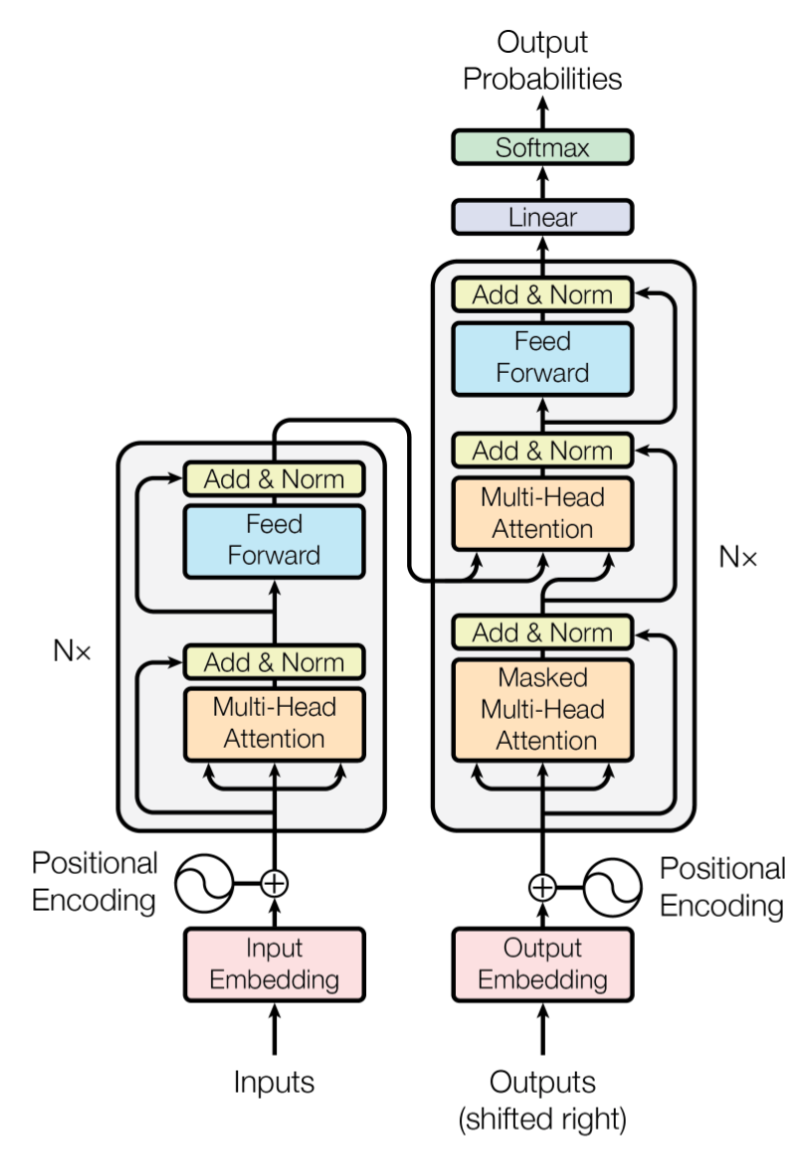
\includegraphics[width=0.45\linewidth]{Images/Transformer_architecture3.png}
    \caption{Transformer Architecture from~\cite{vaswani2017attention}}\label{fig:Tranformer}
\end{figure}

The Transformer is fundamentally structured as an \textit{encoder-decoder} model. The \textbf{encoder} processes the input sequence and produces a continuous vector representation, while the \textbf{decoder} generates the output sequence one token at a time, conditioning on both the encoder output and previously generated tokens. This architecture allows the model to handle input and output sequences at variable length and is the foundation for tasks such as machine translation, summarization, and question answering.

\subsection{Main Innovations in Transformer Architecture}  
\begin{itemize}
    \item \textbf{Embeddings}: Learned embeddings convert input and output tokens to vectors of dimension $d$ depending on the dimension of the model. Tokens are discrete symbols of words or subwords.
    
    \item \textbf{Positional Coding}:  
    Transformers do not need recurrence nor convolution, instead some information about relative or absolute position of the tokens is injected in the sequences. This is the positional encodings added to the input embeddings. \cite{vaswani2017attention}.
    
    \item \textbf{Layer Normalization}: Applied after attention and feed-forward layers (or before, in pre-norm variants), layer normalization stabilizes training by normalizing activations to zero mean and unit variance. It is essential for enabling deep stacking of transformer blocks without training instability.  
    \item  \textbf{Scaled Dot-Product Attention} \ref{eq:Attention}: Is an attention function \ref{eq:Attention} that maps a query and a set of key-value pairs to an output.
    \begin{equation}
        \label{eq:Attention}
        \text{Attention}(Q,K,V) = softmax(\frac{QK^T}{\sqrt{d_k}})V 
    \end{equation}
    The scaling factor $\sqrt{d_k}$ prevents gradient vanishing in attention weights: without it, large dot products would lead to very small gradients after softmax. This stabilizes training and allows for better gradient flow during backpropagation.
    \begin{itemize}
        \item Q is a set of queries packed together into a matrix.
        \item K and V are also matrices packed together of keys and values, respectively
    \end{itemize}
    \item \textbf{Multi-Head Attention}:  Queries, keys and values are linearly projected $h$ different times with different learned linear projections\ref{eq:MultiHead}. Multiple attention heads allow the model to jointly attend to information from different representation subspaces at different positions, enabling simultaneous focus on syntactic and semantic features. This is more effective than a single large attention head.
    \begin{equation}
        \label{eq:MultiHead}
        \text{MultiHead}(Q,K,V) = \text{Concat}(head_1, ..., head_h)W^O  
    \end{equation}
    \begin{itemize}
        \item $head_i = \text{Attention}(QW_i^Q, KW_i^K,VW_i^V)$
    \end{itemize}
    
    \item \textbf{Residual Connections}: Skip connections are placed around both the attention and feed-forward sub-layers, allowing gradients to flow directly through the network. This is critical for training very deep models, as it mitigates the vanishing gradient problem and enables stable learning of identity mappings.

    \item \textbf{Feed-Forward}:  A Position-Wise Feed-Forward Network (FFN) \ref{eq:FNN} is a fully connected neural network designed to independently process each position in the sequence.  While FNN \ref{eq:FNN} operates identically at all positions, the parameters vary between layers. The dimension of the inner-layer has a larger dimension than the model's dimension to increase its capacity to learn complex transformations~\cite{vaswani2017attention}.
    \begin{equation}
        \label{eq:FNN}
        \text{FNN}(x) = \max(0,xW_1+b_1)W_2+b_2
    \end{equation}
\end{itemize}

\subsection{Self-Attention vs. Cross-Attention}
While the attention mechanism described above is \textit{self-attention}—where queries, keys, and values all come from the same sequence—the Transformer decoder also employs \textit{cross-attention}. In cross-attention, queries come from the decoder's previous layer, while keys and values come from the encoder output. This allows the decoder to attend to relevant encoder representations when generating each output token, forming the crucial bridge between encoded input and generated output in tasks like machine translation.

\subsection{Connection to Modern Language Models}  
The Transformer architecture achieved top results in machine translation tasks, such as on the WMT 2014 English-German and English-French datasets, with significantly shorter training times compared to previous models that relied on recurrent architectures. For example, the model achieved a BLEU score of 28.4 on English-to-German translation, outperforming previous architectures by more than 2 BLEU points \cite{vaswani2017attention}.

While the original Transformer used both encoder and decoder, subsequent adaptations have proven remarkably versatile: \textit{encoder-only} models like \gls{BERT} leverage masked self-attention for deep bidirectional understanding, while \textit{decoder-only} models like \gls{GPT} stack self-attention layers to autoregressively generate text one token at a time. These architectural variants, combined with massive pretraining on diverse text corpora, form the foundation of modern \glsxtrfullpl{LLM}. The Transformer's core principles of self-attention and scalability have thus enabled the current era of large language models.

\section{\glsxtrfull{LLM}}
\label{sec:llm}
Building on the Transformer architectures described in Section~\ref{sec:transformer}, modern \glsxtrfullpl{LLM} like \gls{BERT} and \gls{GPT} have become the foundation for advanced \glsxtrfull{NLP} tasks. Summarization and reasoning are key capabilities of \glsxtrfull{AAI} systems, which must distill context, interpret complex instructions, and generate coherent responses. This section focuses on the practical choice of \gls{LLM} provider for this thesis.

While open-source models such as LLaMA, Mistral, and Falcon (available via Hugging Face) offer valuable baseline options, this thesis primarily utilizes the OpenAI API. Compared to hosting open-source models on local servers, OpenAI's approach is cheaper, higher-performing, and more scalable, since it removes infrastructure costs while providing access to cutting-edge systems like \gls{GPT}-4o and \gls{GPT}-4o-mini.

Strong empirical evidence supports the OpenAI choice, even for Portuguese language tasks:
\begin{itemize}
  \item On the Brazilian ENEM entrance exam, \gls{GPT}-4 with Chain-of-Thought prompting achieved 87\% accuracy, surpassing \gls{GPT}-3.5 by 11 points \cite{arxiv2303.17003}.
  \item On the Portuguese National Medical Residency Access Examination, \gls{GPT}-4o outperformed LLaMA 3.1 by 7–11\% across medical domains \cite{pmc12166901}.
\end{itemize}

Given these performance advantages, even performing well in the Portuguese language, along with cost-effectiveness and scalability, OpenAI \glspl{LLM} are adopted in this thesis as the principal agents for reasoning and summarization.


\section{\glsxtrfull{RAG}}
\label{sec:rag}

(\glsxtrfull{RAG}) is a framework designed to improve performance on knowledge-intensive \gls{NLP} tasks. It combines \textit{parametric knowledge}, implicitly stored in the parameters of a pre-trained \glsxtrfull{LLM}, with \textit{non-parametric knowledge}, retrieved from external sources such as document collections or databases. Traditional \glsxtrfullpl{LLM} encode knowledge implicitly in their parameters, which is static, cannot be updated without retraining, and may become outdated. \gls{RAG} mitigates this limitation by introducing a retrieval component that accesses external, explicit, and up-to-date information. Instead of relying solely on the static internal knowledge of the model, RAG enhances generation with dynamically retrieved and contextually relevant information.

\subsection{RAG Pipeline Architecture}
A typical RAG pipeline operates in three sequential stages: (1) \textbf{Retrieval}, where the system searches an external knowledge base (e.g., a vector database) to retrieve the most relevant documents or passages given an input query; (2) \textbf{Augmentation}, where the retrieved documents/chunks of text are then combined with the query to form an enriched prompt, providing the \gls{LLM} with additional context; and (3) \textbf{Generation}, where the \gls{LLM} conditions its output on both the query and the retrieved context, producing responses from known sources. To use AI for semantic search effectively, it is essential to use \gls{RAG} to ensure access to up-to-date information.

\subsection{Retrieval Methods in RAG}

The retrieval stage can be implemented in multiple ways, ranging from traditional sparse methods to modern dense retrieval techniques. This subsection covers both approaches.

\subsubsection{Sparse Retrieval Methods}

Traditional sparse retrieval approaches rely on \textbf{sparse representations}, where documents are represented as bags of words or weighted keyword vectors. These are sparse vector space models that match keywords efficiently via an inverted index, representing both queries and documents as high-dimensional, sparse vectors with term-based weighting. While these models are often effective for keyword-based matches, they struggle when queries and relevant documents use synonyms or paraphrases that do not share surface-level terms.

Well-known sparse retrieval methods include TF-IDF and BM25, which are detailed below.

\paragraph{TF-IDF (Term Frequency-Inverse Document Frequency)}

TF-IDF is a foundational term-weighting and ranking scheme in information retrieval systems \cite{tf-idf}. Its primary purpose is to measure how important a term is to a particular document within a large collection of documents. While frequency counts can highlight terms that often appear, they do not account for how common or rare those terms are across the entire dataset. TF-IDF addresses this by diminishing the weight of terms that occur frequently across many documents and increasing the weight of terms that appear in fewer documents (more distinctive terms).

The \glsxtrfull{TF} measures how often a term \textit{t} appears in a single document \textit{d}:
\begin{equation}
    \label{eq:tf} 
    \text{TF}(t,d)=f_{t,d}
\end{equation}
where $f_{t,d}$ is the frequency of term $t$ in document $d$.

For longer documents, a normalization is applied:
\begin{equation}
    \label{eq:tf(t,d)}
    \text{TF}(t,d) = \frac{f_{t,d}}{\sum_{t'}f_{t',d}}
\end{equation}

The inverse document frequency (IDF) measures how common a term is across the entire collection of documents. If a term appears in many documents, it is less useful for distinguishing those documents. A higher IDF means a term appears in fewer documents, indicating its uniqueness. Let \textit{N} be the total number of documents in the collection, and $n_t$ be the number of documents in which the term appears. \textit{IDF} is defined as:
\begin{equation}
    \label{eq:idftf}
    \text{IDF}(t)=\log\frac{N}{n_t}
\end{equation}

TF-IDF is then the combination of both TF and IDF:
\begin{equation}
    \label{eq:tfidf}
    \text{TF-IDF}(t,d) = f_{t,d} \times \log\left(\frac{N}{n_t}\right)
\end{equation}

The uniqueness of the TF-IDF approach in retrieval is how it combines a local component (frequency in the current document) and a global component (frequency across the entire collection). TF-IDF has the advantage of being straightforward, interpretable, and computationally efficient.

\paragraph{BM25 (Okapi BM25)}

The Okapi BM25 system, first introduced in \cite{Bm25foundation}, culminated in BM25 (short for ``Best Match 25''), a probabilistic information retrieval model. BM25 improves upon TF-IDF by using a probabilistic basis rather than a purely heuristic one, and by introducing parameters to control term frequency saturation and document length normalization.

The BM25 formula is similar to TF-IDF in structure, but uses a more sophisticated formulation of the IDF component that is more stable and empirically effective. The IDF component per term \textit{t} is computed as:
\begin{equation}
    \label{eq:idfbm25}
    \text{IDF}(t) = \log \frac{N-n_t+0.5}{n_t+0.5}
\end{equation}
where N is the total number of documents in the collection and $n_t$ is the number of documents containing term \textit{t}.

The BM25 formula to score a document $d$ given a query $q$ (consisting of multiple terms) is:
\begin{equation}
    \label{eq:bm25}
    \textit{BM25}(d,q) = \sum_{t \in q} \text{IDF}(t) \cdot \frac{(k_1+1)\cdot f_{t,d}}{f_{t,d}+k_1(1-b+b \cdot \frac{|d|}{avgdl})}
\end{equation}
where:
\begin{itemize}
\item $d$ is a given document.
\item $q$ a user's query, consisting of terms.
\item $|d|$ is the length of a document in terms of the number of tokens.
\item $avgdl$ is average document length across the entire collection.
\item $k_1$ and $b$ are tuning parameters:
\begin{itemize}
    \item $k_1$ controls the saturation of \glsxtrfull{TF}, by preventing over-emphasis on very frequent terms.
    \item $b$ controls document length normalization. If $b = 1$, the normalization is directly proportional to how much longer (or shorter) the document ($|d|$) is compared to average document length ($avgdl$). If $b=0$, no document length normalization is applied.
\end{itemize}
\end{itemize}

\subsubsection{Dense Retrieval Methods}

Recent advancements in \gls{LLM}, particularly transformer-based models like \gls{BERT} \cite{bertpretrainingdeepbidirectional}, have led to dense retrieval systems that overcome the limitations of sparse methods. In dense retrieval, queries and documents are represented as low-dimensional vectors that better capture semantic similarity. However, dense methods often require large training datasets (i.e., labeled question–passage pairs) to surpass classical methods such as TF-IDF/BM25. Modern pre-trained language models help mitigate this requirement by providing robust initial embeddings that can be fine-tuned on relatively smaller sets of question–context examples, enabling dense retrieval methods to outperform traditional sparse approaches in many open-domain QA tasks.

\paragraph{Dense Passage Retrieval (DPR)}
\label{par:dpr}

Dense Passage Retrieval (DPR), introduced by Karpukhin et al.~\cite{densepassageretrievalopendomainkarpukhin2020}, is a \textit{dense retrieval} method designed specifically for \textit{open-domain question answering}. Unlike conventional approaches that rely on \textit{purely lexical} matches (e.g., TF-IDF and BM25), DPR employs \gls{BERT}-based encoders to map questions and passages into a shared, dense embedding space, enabling \textit{semantic} rather than strictly \textit{keyword-based} retrieval. By leveraging modern \gls{LLM} such as \gls{BERT}~\cite{bertpretrainingdeepbidirectional} and LLaMA, which come with strong pre-trained representations, DPR can be fine-tuned with comparatively fewer labeled samples. This allows the system to capture semantic relationships between questions and passages, thereby mitigating the shortcomings of traditional methods that rely solely on term overlap.

The DPR architecture is based on a dual-encoder architecture~\cite{dualencoderarchitecture}. Specifically, in Karpukhin et al.'s formulation~\cite{densepassageretrievalopendomainkarpukhin2020}, both encoders are initialized from the same pre-trained \gls{BERT} model but are then fine-tuned separately for their respective tasks. A Question Encoder \(E_Q\) takes a question as input and produces a single vector embedding \(\mathbf{q_i}\), while a Passage Encoder \(E_P\) processes a passage to produce a single vector embedding \(\mathbf{p_j}\). Once encoded, each question and passage becomes a fixed-dimensional vector (e.g., 768 dimensions). To measure the similarity between a question \((\mathbf{q})\) and a passage \((\mathbf{p})\), the dot product of their embeddings is computed:
\begin{equation}
    \label{eq:dot_sim}
    \text{similarity}(\mathbf{q}, \mathbf{p}) = E_Q(\mathbf{q})^T \, E_P(\mathbf{p})
\end{equation}
where $\mathbf{q}$ is the question embedding and $\mathbf{p}$ is the passage embedding, both produced by their respective encoders.

\section{Sentence Transformers}
\label{sec:Sentence-Transformers}
Sentence Transformers are \gls{BERT}-based encoder models designed to generate dense vector representations (embeddings) of entire sentences or passages. 
They were introduced in 2019 \cite{reimers2019sentencebertsentenceembeddingsusing} as an adaptation of the \gls{BERT} architecture, which was originally built for token-level classification tasks.

With the use of Siamese and Triplet network structures on top of \gls{BERT}, SBERT modifies the architecture to operate at the sentence level. Instead of encoding a pair of sentences jointly, as in the cross-encoder setup of standard \gls{BERT}, SBERT processes each sentence independently with a shared \gls{BERT} encoder. This produces fixed-size embeddings that can later be compared directly using cosine similarity or other distance metrics, making large-scale similarity search computationally feasible.

In a Siamese setup, two identical \gls{BERT} encoders with shared weights process different input sentences. Their embeddings are then compared, allowing the network to learn similarity or classification objectives. This design ensures that semantically similar sentences are mapped to nearby points in the embedding space, while dissimilar ones are pushed apart.

Triplet networks extend this idea by processing three inputs simultaneously: an anchor sentence, a positive sentence with similar meaning, and a negative sentence with unrelated meaning. The model is trained to minimize the distance between the anchor and the positive embedding, while maximizing the distance between the anchor and the negative embedding. This objective directly enforces a semantically meaningful structure in the embedding space, making the representations more robust for tasks such as \glsxtrfull{STS} and information retrieval.
\begin{figure}[h!]
    \centering
    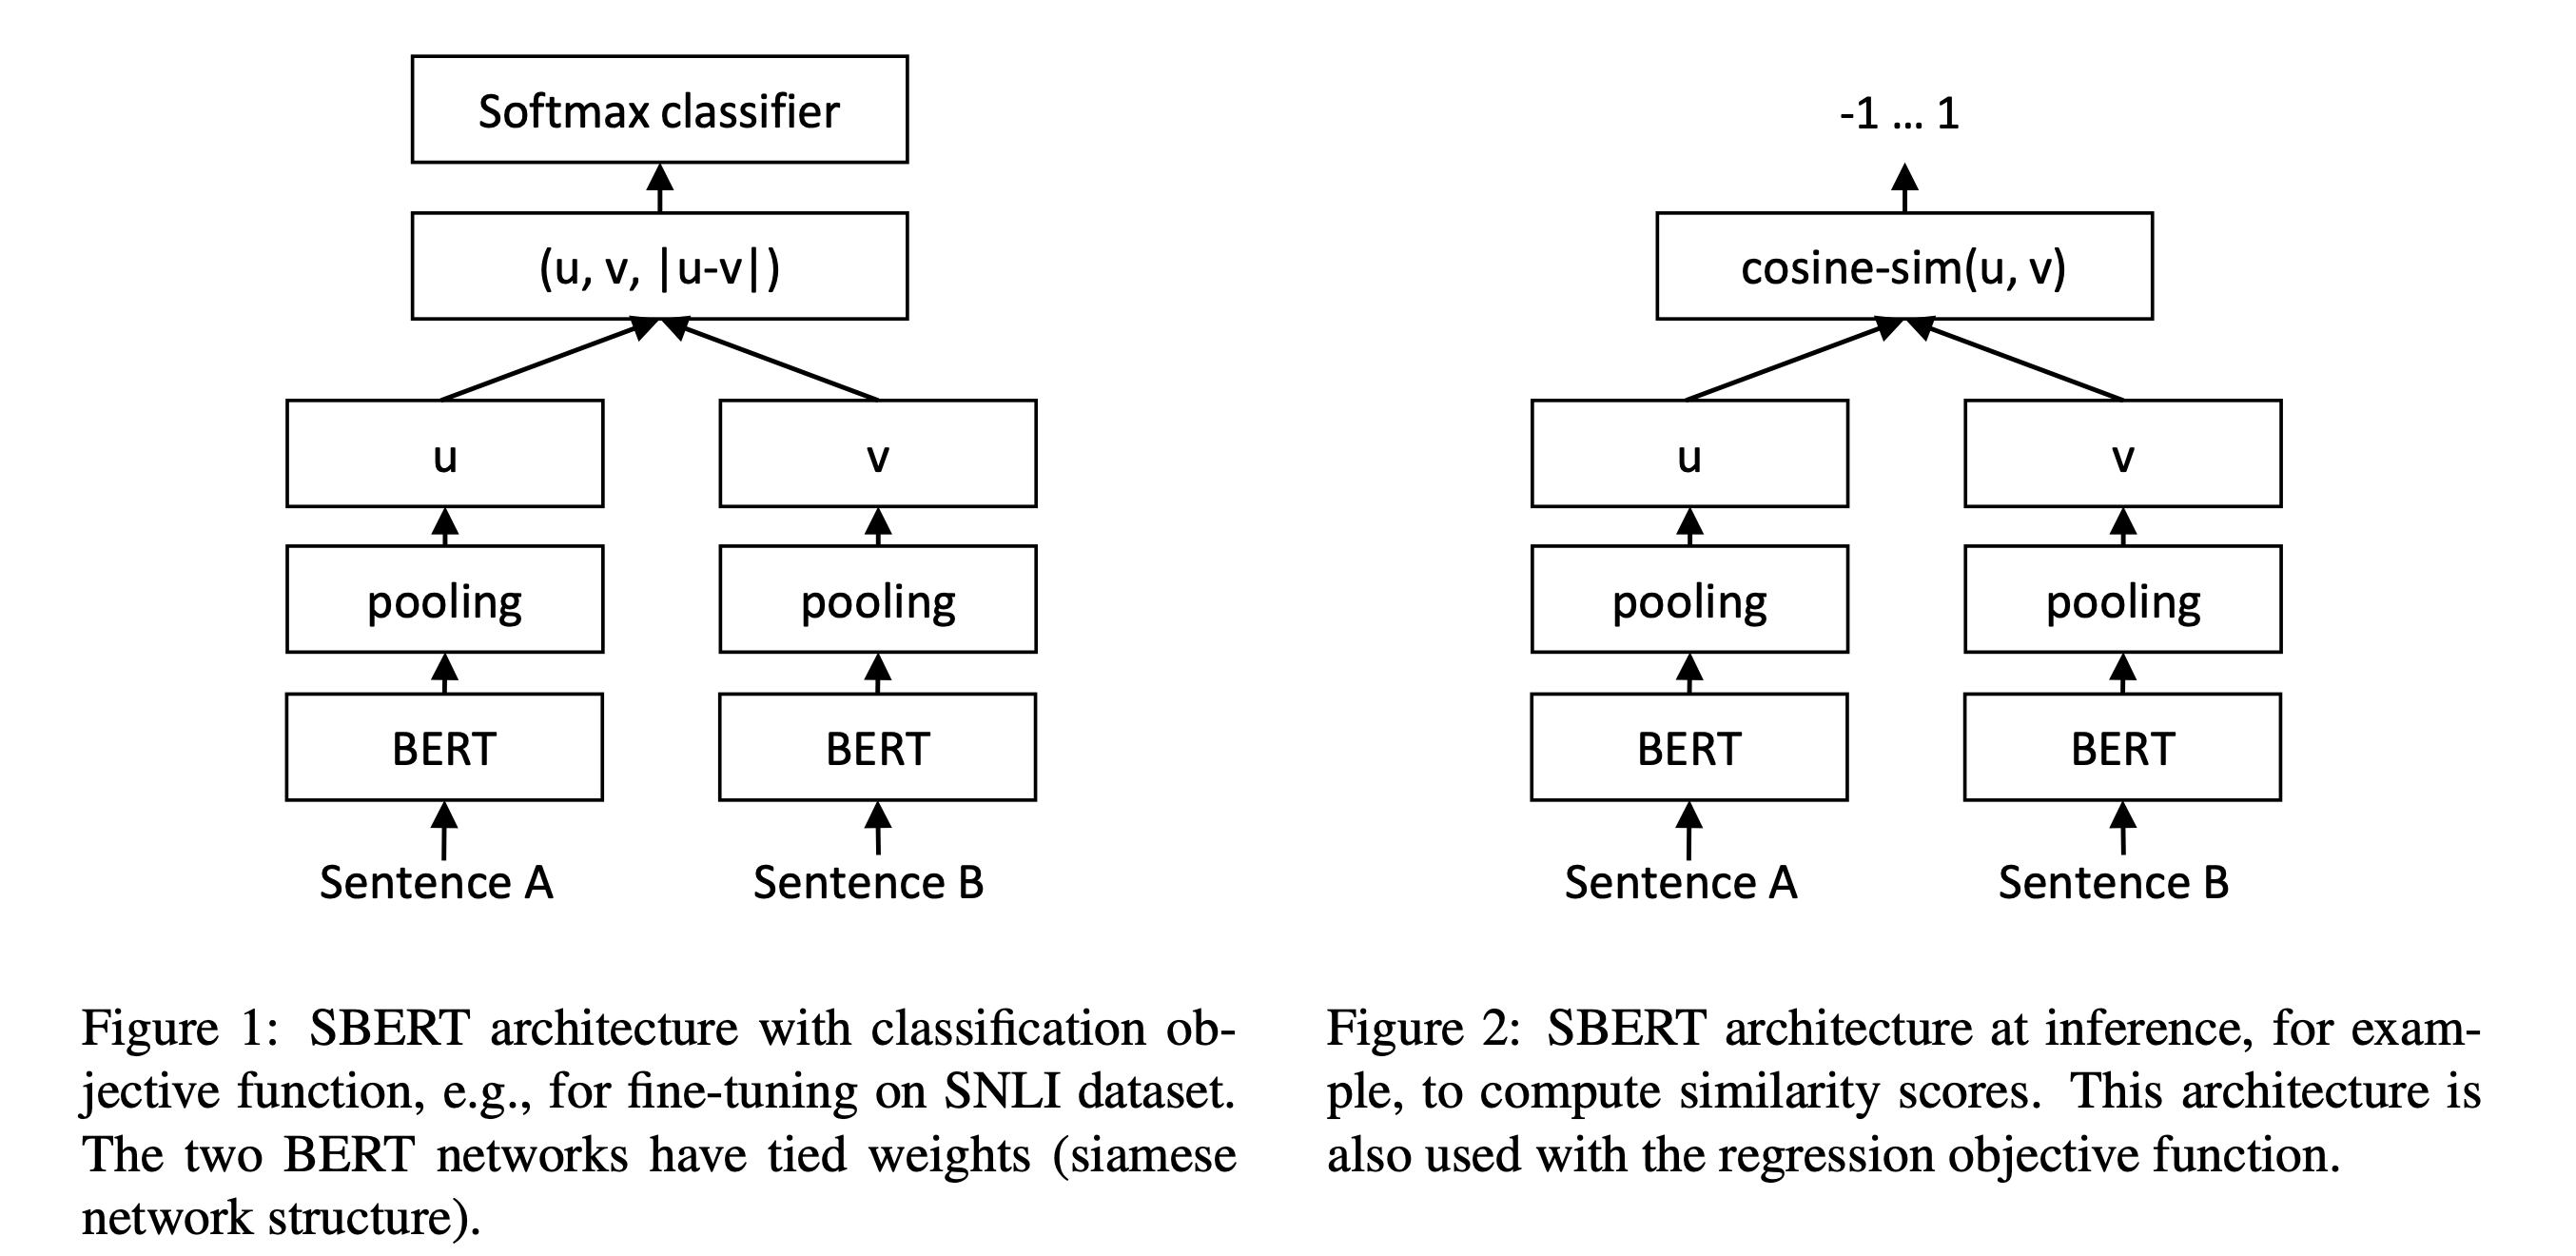
\includegraphics[width=1\linewidth]{Images/sentence_transformer.png}
    \caption{Sentence Transformer Architecture explained in~\cite{reimers2019sentencebertsentenceembeddingsusing}}
    \label{fig:sentence-transformer-architecture}
\end{figure}
Since \gls{BERT} outputs contextual embeddings for individual tokens, an additional pooling layer is required to derive a single sentence vector, as shown in Figure~\ref{fig:Sentence_embedding}. In \cite{reimers2019sentencebertsentenceembeddingsusing}, the preferred pooling method for \gls{STS} tasks is mean pooling, which turns multiple token embeddings into a single sentence embedding.\footnote{Other pooling strategies, such as using the \texttt{[CLS]} token or max pooling, were also evaluated but performed worse for semantic similarity tasks.}

\begin{figure}[h!]
    \centering
    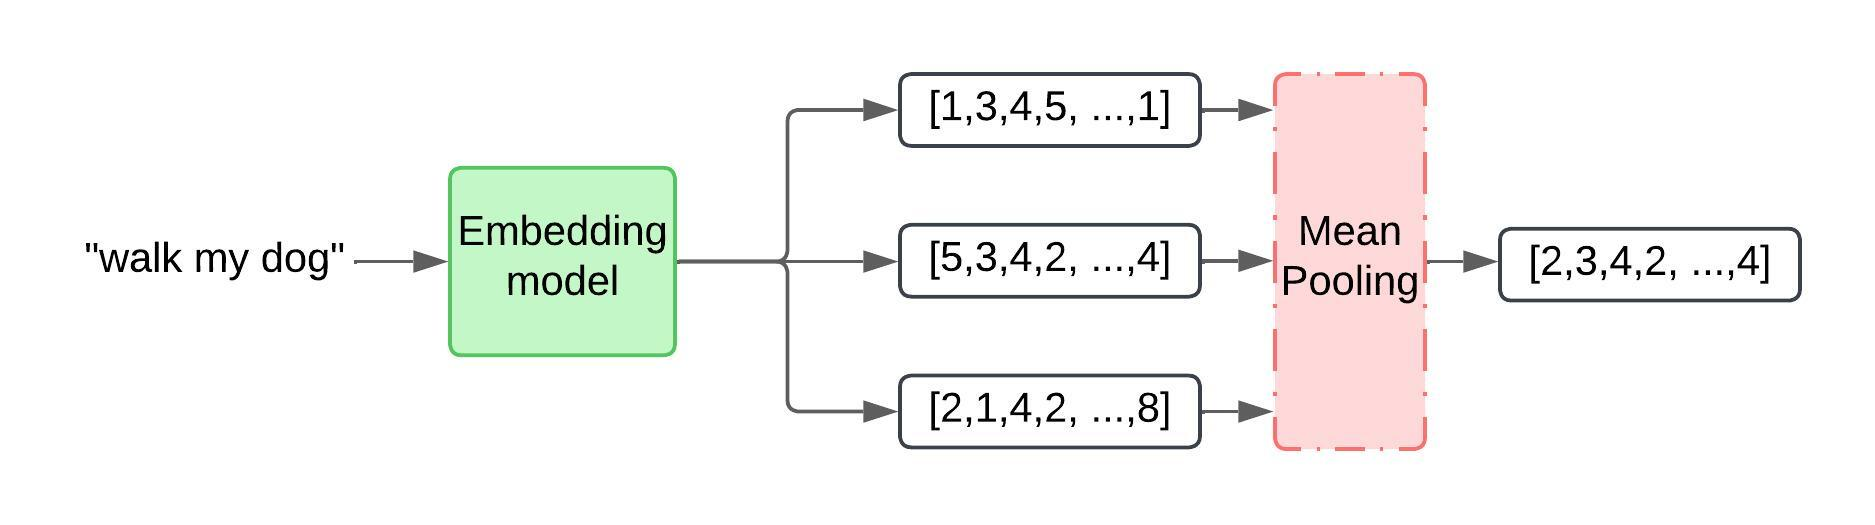
\includegraphics[width=1\linewidth]{Figures/Sentence_Embedding.jpeg}
    \caption{Example illustration of sentence embedding through mean pooling.}\label{fig:Sentence_embedding}
\end{figure}

To ensure that these embeddings capture sentence-level meaning, SBERT is fine-tuned on tasks such as (\gls{NLI}), (\gls{STS}), and triplet training. 

When trained on \gls{NLI} data with a classification objective, SBERT further compares pairs of sentence embeddings by constructing a combined feature vector $(u, v, |u-v|)$, where $u$ and $v$ are the pooled embeddings of the two sentences. This representation proved effective in downstream tasks such as the Semantic Textual Similarity benchmark (\gls{STS}-b).

The quality of a Sentence Transformer is ultimately reflected in the accuracy and robustness of the embeddings it produces. Recent research has extended these methods to Portuguese, with the current state-of-the-art being the \textit{Serafim 900M IR} model \cite{gomes2024opensentenceembeddingsportuguese}, which has been specifically trained and benchmarked for \gls{STS} and \gls{IR} tasks.

\section{Vector Databases}
\label{sec:vector-store}
As described in more detail Section~\ref{sec:Sentence-Transformers}, embedding models transform unstructured data (e.g., text, images, or audio) into high-dimensional numerical vectors that capture semantic relationships. In such a vector space, similar objects are positioned closer together, while unrelated ones are placed farther apart. For example, the terms \emph{dog} and \emph{wolf} would be embedded near each other, whereas \emph{banana} would appear in a distant region (see Fig.~\ref{fig:vector-embedding}).  

A vector database stores these embeddings and supports efficient similarity search through vector indexing techniques, enabling similarity search at scale.
\begin{figure}[h]
    \centering
    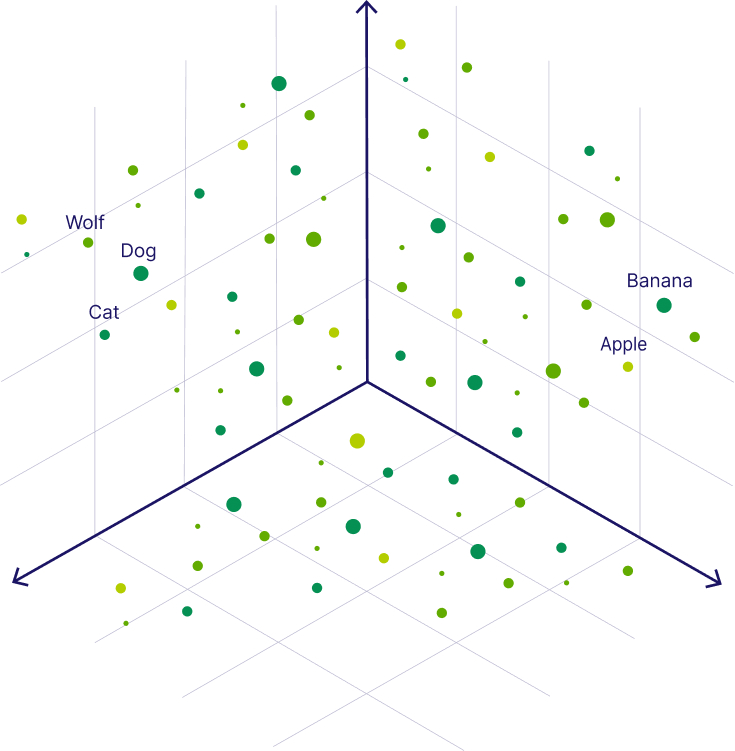
\includegraphics[width=0.55\linewidth]{Images/vector-embedding.jpg}
    \caption{Example of vector embeddings where semantically related terms are placed closer in the vector space \cite{weaviate}}
    \label{fig:vector-embedding}
\end{figure}

During inference, vector databases enable fast retrieval of relevant embeddings using Approximate Nearest Neighbor (\glsxtrfull{ANN}) search. 
Indexing algorithms such as \glsxtrfull{HNSW}, \gls{IVF}, Product Quantization (PQ), or \gls{ANNOY} are commonly employed. 
These methods differ in how they organize the search space: 
\gls{HNSW} constructs a hierarchical graph, which supports dynamic insertion of new vectors and logarithmic-time search, making it suitable for continuously growing datasets. 
\gls{ANNOY} builds static random-projection trees that are optimized for read-heavy workloads, but generally require index rebuilding when new vectors are added. 
\gls{IVF} partitions the vector space into clusters and restricts search to the most relevant clusters, which reduces query time at the cost of some recall. 
PQ compresses vectors into smaller codewords, drastically reducing memory consumption while enabling efficient approximate similarity computations. 

Figure~\ref{fig:semantic-search-pipeline} illustrates the flow from raw data to evaluation: embeddings are indexed using \gls{ANN} algorithms and queried using a vector representation of the input. The retrieved results are then evaluated using similarity metrics \ref{sec:vector-similarity}
\begin{figure}[H]
    \centering
    \begin{tikzpicture}[
        node distance=1.7cm and 2.2cm,
        every node/.style={font=\small, align=center},
        process/.style={rectangle, draw=black, rounded corners, minimum height=1.1cm, minimum width=2.8cm},
        arrow/.style={->, thick}
    ]
        % Nodes
        \node[process] (input) {Unstructured Data \\ (Text, Image, Audio)};
        \node[process, right=of input] (embed) {Embedding Model \\ (e.g., SBERT)};
        \node[process, right=of embed] (index) {Vector Database \\ + ANN Index (e.g., HNSW)};
        \node[process, below=of index] (query) {Query Embedding};
        \node[process, left=of query] (retrieval) {Nearest Neighbors \\ (Top-K Retrieval)};
        \node[process, below=of retrieval] (metrics) {Similarity Metrics \\ (Cosine, Dot, Euclidean)};

        % Arrows
        \draw[arrow] (input) -- (embed);
        \draw[arrow] (embed) -- (index);
        \draw[arrow] (query) -- (index);
        \draw[arrow] (index) -- (retrieval);
        \draw[arrow] (retrieval) -- (metrics);
    \end{tikzpicture}
    \caption{Semantic retrieval pipeline: data is embedded, indexed, and queried using vector similarity search. Retrieved vectors are then evaluated using similarity metrics.}\label{fig:semantic-search-pipeline}
\end{figure}

\subsection{HNSW: Hierarchical Navigable Small World Graph}

\glsxtrfull{HNSW}~\cite{malkov2018efficient} is a graph-based indexing algorithm widely used in vector databases for approximate nearest neighbor (\gls{ANN}) search. It is based on the principle of small-world networks, where most nodes can be reached in a small number of steps, despite the overall network being large.

\begin{itemize}
    \item \textbf{Graph Construction.} HNSW builds a multi-layer graph where each layer is a proximity graph: nodes (vectors) are connected to their closest neighbors according to a similarity metric (e.g., cosine similarity or Euclidean distance). The top layers have fewer nodes and longer links, forming a hierarchical structure. New vectors are inserted from the top layer down to the bottom, gradually establishing local connections at each level.

    \item \textbf{Search Process.} The search begins at the topmost layer and navigates greedily toward the query vector by moving to the closest neighbor at each step. Once a local minimum is reached, the process descends to the next layer and repeats, refining the search as it approaches the bottom layer (the densest one). The final result is a list of approximate nearest neighbors from the base layer.

    \item \textbf{Time and Space Complexity.} HNSW offers logarithmic search complexity—$\mathcal{O}(\log N)$ in practice—and supports dynamic insertion of vectors, unlike many tree-based or clustering-based methods. It requires additional memory for storing the graph structure, but in return provides excellent trade-offs between recall, latency, and update support.
\end{itemize}

Compared to other indexing methods such as IVF or ANNOY, HNSW tends to achieve higher recall at lower latency, especially in scenarios where index updates are frequent or low-latency responses are critical. Due to these properties, HNSW is the default index used in several vector databases such as FAISS, Milvus, and Weaviate.

\subsection{Vector Similarity}
\label{sec:vector-similarity}
The similarity between vectors can be computed using several distance or similarity metrics, which are also employed in later semantic evaluation tasks with metrics such as:

\begin{itemize}
    \item \textbf{Cosine similarity:} computes the cosine of the angle between two vectors. It is invariant to magnitude, making it useful when semantic meaning is encoded in direction rather than length:  
    \[
        \textit{cos\_sim}(\mathbf{u}, \mathbf{v}) = \frac{\mathbf{u} \cdot \mathbf{v}}{\|\mathbf{u}\| \, \|\mathbf{v}\|}
    \]
    
    \item \textbf{Euclidean distance:} computes the straight-line distance between two vectors in the embedding space. It is effective when similarity correlates with geometric closeness:  
    \[
        d_{\textit{euclidean}}(\mathbf{u}, \mathbf{v}) = \|\mathbf{u} - \mathbf{v}\|_2 = \sqrt{\sum_{i=1}^n (u_i - v_i)^2}
    \]
    
    \item \textbf{Dot product:} measures the projection of one vector onto another, capturing both direction and magnitude. It is frequently employed in large-scale retrieval systems to approximate inner products between compressed vectors:  
    \[
        \textit{dot}(\mathbf{u}, \mathbf{v}) = \sum_{i=1}^n u_i v_i
    \]
\end{itemize}


Vector databases exist across a spectrum of complexity. Full-featured systems such as Weaviate, Pinecone, and Milvus provide distributed storage, hybrid queries, and built-in integrations with embedding providers.


\section{Text Summarization}
\label{sec:text-summarization}

Text summarization is a critical task in natural language processing that condenses lengthy documents into shorter, coherent representations while preserving essential information. In the context of (\gls{RAG}), summarization serves multiple purposes: it can compress retrieved passages to reduce context length, distill key information for the \gls{LLM} to reason over, and ensure that generated responses are grounded in the most relevant content.

Summarization approaches are broadly categorized into two types: \textit{extractive} methods, which select existing sentences or phrases from the source text, and \textit{abstractive} methods, which generate new text by understanding and paraphrasing the original content. While extractive summarization is simpler and preserves exact language from the source, abstractive methods can produce more fluent and concise summaries that better reflect the semantic meaning of the original text. This section focuses on \textbf{\gls{BART}}, a state-of-the-art transformer-based model designed specifically for abstractive summarization and other sequence-to-sequence tasks.

\subsection{LexRank: Graph-Based Extractive Summarization}

LexRank, introduced by Erkan and Radev~\cite{erkan2004lexrank}, is a graph-based extractive summarization method, that identifies and ranks the most important sentences in a document. Unlike abstractive methods that generate new text, LexRank operates by selecting sentences that are most representative of the document's content.

The core principle of LexRank is to compute sentence importance based on a concept of \textit{lexical centrality}. Sentences are represented as nodes in a graph, and edges are weighted by the degree of similarity between sentences, typically measured using cosine similarity over TF-IDF vectors. The algorithm then applies PageRank-style centrality computation to identify sentences that are semantically central to the document—that is, sentences that are similar to many other sentences in the document.

The LexRank algorithm operates as follows:

\begin{enumerate}
    \item \textbf{Build Similarity Graph:} Compute pairwise cosine similarities between all sentences using TF-IDF representations. Create an edge between two sentences if their similarity exceeds a predefined similarity threshold.
    
    \item \textbf{Compute Centrality:} Apply a graph centrality algorithm (typically PageRank) to compute the importance of each sentence. Sentences that are central to the graph (well-connected to other sentences) receive higher scores.
    
    \item \textbf{Extract Summary:} Select the top-ranked sentences and arrange them in their original document order to form the summary.
\end{enumerate}

LexRank's strength lies in its simplicity, interpretability, and computational efficiency. Since it is entirely unsupervised and does not require labeled training data, it can be applied to any domain without requiring domain-specific tuning . Furthermore, the graph-based approach naturally captures the thematic coherence of documents by selecting sentences that are representative of the overall content.

However, LexRank has notable limitations. First, as an extractive method, it is constrained to sentences that already exist in the source document, which can result in summaries that are less fluent or concise than abstractive approaches. Second, the method may struggle with documents where important information is distributed across multiple dissimilar sentences, or where key concepts appear in unusual phrasings. Third, LexRank does not explicitly model semantic relationships beyond lexical similarity, potentially missing paraphrases or synonyms that convey the same meaning.

\subsection{BART: Denoising Sequence-to-Sequence Pretraining}

\gls{BART}, introduced by Lewis et al.~\cite{lewis2019bart}, is a sequence-to-sequence transformer model that combines the best aspects of both \gls{BERT} and \gls{GPT}-like architectures. \gls{BART} is pretrained using a denoising objective, where random segments of text in the input are corrupted (masked, deleted, or permuted), and the model learns to reconstruct the original text. This pretraining strategy makes \gls{BART} particularly effective for generation tasks, as it learns to handle both semantic understanding (like \gls{BERT}) and generation (like \gls{GPT}).

\subsubsection{BART Architecture}

The \gls{BART} architecture follows the standard encoder-decoder structure. The \textbf{Encoder} is a \gls{BERT}-like bidirectional transformer that processes the corrupted input and produces contextual representations. The \textbf{Decoder} is an autoregressive transformer (similar to \gls{GPT}) that generates the output sequence token-by-token, attending to both the encoder output and previously generated tokens. Both components use the standard Transformer building blocks (multi-head self-attention, feed-forward networks, layer normalization, and residual connections) as described in Section~\ref{sec:transformer}. The encoder-decoder attention allows the decoder to attend to relevant parts of the encoded input, enabling effective informationtransfer from input to output sequences.

\subsubsection{Denoising Pretraining Objective}

\gls{BART} is pretrained on a denoising task where the input is artificially corrupted in various ways, and the model learns to denoise (reconstruct) the original text. The corruption strategies employed include: \textbf{Token Masking}, where random tokens are replaced with a special \texttt{[MASK]} token, similar to \gls{BERT}; \textbf{Token Deletion}, where random tokens are removed entirely, forcing the model to infer missing information from context; \textbf{Text Infilling}, where spans of consecutive tokens are replaced with a single mask token, requiring the model to generate the complete missing phrase; \textbf{Sentence Permutation}, where the order of sentences in the document is randomly shuffled, and the model learns to reorder them correctly; and \textbf{Document Rotation}, where the document is rotated by removing some initial tokens and moving them to the end, and the model learns to identify the original starting position.

This diverse corruption strategy ensures that \gls{BART} learns robust representations and can handle various downstream tasks. The denoising objective is formally expressed as:

\begin{equation}
    \mathcal{L} = -\log P(x | \text{corrupt}(x))
\end{equation}

where $x$ is the original text, $\text{corrupt}(x)$ is the corrupted version, and the model learns to reconstruct $x$ from the corrupted input.

\subsubsection{Fine-tuning for Summarization}

For abstractive summarization, \gls{BART} is fine-tuned on annotated summarization datasets (e.g., CNN/Daily Mail, XSum), where pairs of documents and their corresponding summaries are available. During fine-tuning, the model learns to map lengthy input documents to concise summary outputs. The fine-tuning objective is:

\begin{equation}
    \mathcal{L}_{\text{summ}} = -\log P(s | d)
\end{equation}

where $d$ is the input document and $s$ is the target summary. The decoder generates the summary\textit{ autoregressively}, one token at a time, conditioned on the encoder representation of the input document.

At inference time, the model generates summaries using beam search or sampling strategies, balancing between diversity and quality. Beam search maintains the top-$k$ most likely hypotheses at each decoding step, selecting the final sequence with the highest probability.

\subsection{Summary}

\gls{BART} suits \gls{RAG} summarization for three reasons. i) superior performance on CNN/Daily Mail and XSum, outperforming T5 and PEGASUS with state-of-the-art ROUGE scores\footnote{The \gls{BART} paper reports ROUGE-2 F1 scores of 21.45 on CNN/Daily Mail and 45.14 on XSum, surpassing comparable T5 and PEGASUS configurations \cite{lewis2019bart}. } ii) efficient GPU deployment with a modest memory footprint (~1.2 GB base; ~2.5 GB large), enabling co-location with embedding models\footnote{GPU memory estimates are based on typical inference measurements with batch size 1 using the Hugging Face Transformers library. Actual memory consumption may vary depending on batch size, sequence length, and hardware configuration. See \texttt{https://huggingface.co/docs/transformers/model\_memory\_anatomy} for detailed memory profiling guidance.}. iii) minimal latency overhead by sharing the same GPU as retrieval, keeping additional cost low while meeting strict latency budgets.

% Other summarization methods exist in the literature, including TextRank \cite{mihalcea2004textrank}, LexRank \cite{erkan2004lexrank}, SumBasic \cite{vanderwende2007sumbasic}, PEGASUS \cite{zhang2019pegasus}, T5 \cite{raffel2020exploring}, FLAN-T5 \cite{wei2021finetuned}, mBART \cite{tang2020multilingual}, and UniLM \cite{dong2019unified}, though these typically do not match \gls{BART}'s performance on standard benchmarks.

While \gls{BART} excels on benchmarks, extractive LexRank offers two key benefits for \gls{RAG} systems. i) hallucination prevention by preserving source text. ii) storage optimization by keeping only salient sentences, reducing embeddings stored in the \gls{VD}.

Practically, we pair the methods to balance their complementary trade-offs. LexRank preserves factuality and reduces storage by selecting source sentences, but being extractive it can leave context gaps that hinder \gls{LLM} reasoning. \gls{BART} produces context-rich, readable summaries that bridge those gaps, but it may hallucinate. 

\section{Text Similarity Metrics}
\label{sec:text-similarity-metrics}
Since this thesis aims to enhance semantic search through Retrieval-Augmented Generation (\gls{RAG}), 
evaluating similarity between texts becomes a critical component for assessing the model and methodology. 
No single metric fully captures the notion of similarity: some emphasize exact lexical overlap, 
while others account for structural variation or semantic equivalence. 
Therefore, a diverse set of metrics is employed to provide a more comprehensive assessment, 
ensuring that the evaluation reflects the multifaceted nature of semantic search.

\subsection{Evaluation Metrics}

Since this thesis focuses on enhancing semantic search through \gls{RAG}, the evaluation of similarity between retrieved passages, generated answers, and gold references is a crucial step in evaluation. Different metrics capture complementary aspects of similarity, ranging from exact lexical overlap to semantic equivalence. Using a diverse set of metrics ensures that evaluation does not rely on a single definition of similarity, but instead reflects the multifaceted nature of semantic search.
\subsubsection{Binary Matching}
Exact match and substring match are both binary identification methods. Exact Matchchecks if both texts are exactly the same. Substring match check if the gold reference is in the answer. These metrics are fast and simple, but very lexically strict.

\subsubsection{Token Recall} 
Token Recall measures the proportion of reference tokens covered by the prediction:
\[
\text{Recall} = \frac{|A \cap G|}{|G|}
\]
where \(A\) and \(G\) denote the token sets of the answer and reference.  

\subsubsection{Jaccard Similarity} 
Introduced by Jaccard \cite{jaccard1901distribution}, this metric is defined as
\[
J(A,B) = \frac{|A \cap B|}{|A \cup B|}
\]
with \(A\) and \(B\) as token sets.  

\subsubsection{Levenshtein Similarity} 
Based on the edit distance proposed by Levenshtein \cite{levenshtein1966binary}, it is given by
\[
1 - \frac{\text{ED}(A,B)}{\max(|A|,|B|)}
\]
where \(\text{ED}\) is the edit distance between token sequences.  
\footnote{Edit distance is defined as the minimum number of operations (insertions, deletions, or substitutions of tokens) required to transform one sequence into the other.(e.g., transforming “cat sat” into “the cat” requires one insertion and one deletion)}

\subsubsection{ROUGE-n} 
Introduced by Lin \cite{lin2004rouge}, ROUGE measures n-gram overlap between candidate and reference. 
\footnote{An \emph{n-gram} is a contiguous sequence of \(n\) tokens from a text; for example, for the sentence ``the cat sat'', the unigrams (\(n=1\)) are {the, cat, sat}, while the bigrams (\(n=2\)) are {the cat, cat sat}.
ROUGE-1 therefore evaluates unigram overlap, while ROUGE-2 evaluates bigram overlap, which captures short phrase structure in addition to individual words. }
For n-grams of size \(n\), the metric is defined as:
\[
\text{Precision} = \frac{\text{overlap}}{\text{n-grams}(A)}, \quad
\text{Recall} = \frac{\text{overlap}}{\text{n-grams}(B)}, \quad
F1 = \frac{2PR}{P+R}
\]

\subsubsection{\gls{BERT}-based Cosine Similarity.} 
This metric employs dense sentence embeddings from \textit{SentenceTransformer all-MiniLM-L6-v2} \cite{reimers2019sentence}. 
Similarity is computed as cosine similarity:
\[
\cos(\theta) = \frac{v \cdot u}{\|v\| \, \|u\|}
\]

\subsubsection{Overlap Coefficient.} 
Also known as the Szymkiewicz--Simpson coefficient \cite{simpson1960similarity}, it is defined as
\[
\text{Overlap}(A,B) = \frac{|A \cap B|}{\min(|A|,|B|)}
\]

\subsubsection{BLEU.} 
Introduced by Papineni et al. \cite{papineni2002bleu}, BLEU computes modified n-gram precision with a brevity penalty:
\[
\text{BLEU} = \text{BP} \cdot \exp\left(\sum_{n=1}^{N} w_n \log p_n\right)
\]
where \(p_n\) are modified n-gram precisions, \(w_n\) are weights, and BP is the brevity penalty.

By combining these metrics, the evaluation captures complementary perspectives:  
lexical accuracy (Exact Match, Substring, Jaccard), structural similarity (Levenshtein, ROUGE, BLEU), coverage of reference information (Token Recall, Overlap coefficient), and semantic equivalence (\gls{BERT} cosine).This multidimensional evaluation approach allows for a comprehensive assessment by testing both surface-level metrics and deeper semantic understanding.

\section{Youden's J Statistic}
\label{sec:youden}
Youden's J statistic, also known as Youden's index, is a summary measure of the performance of a binary classification test~\cite{youden1950index}. It is defined as:
\[
J = \text{Sensitivity} + \text{Specificity} - 1
\]
where:
\begin{itemize}
    \item \textbf{Sensitivity} (True Positive Rate) is the proportion of actual positives correctly identified.
    \item \textbf{Specificity} (True Negative Rate) is the proportion of actual negatives correctly identified.
\end{itemize}
Youden's J statistic ranges from -1 to 1, where:
\begin{itemize}
    \item A value of 1 indicates a perfect test with no false positives or false negatives.
    \item A value of 0 indicates a test that performs no better than random chance.
    \item A negative value indicates a test that performs worse than random chance.
\end{itemize}
Youden's J statistic is particularly useful for evaluating diagnostic tests and classifiers, as it provides a single metric that balances sensitivity and specificity. It is often used to determine the optimal cutoff point for a test, where the sum of sensitivity and specificity is maximized~\cite{fluss2005youden}.
In the context of this thesis, Youden's J statistic is employed to evaluate the performance of (\gls{RAG}) systems, particularly in scenarios where both false positives and false negatives have significant implications. By maximizing Youden's J, the system can achieve a balance between correctly retrieving relevant information and minimizing the retrieval of irrelevant data.
\section{Summary}
This chapter established the foundations of retrieval in modern intelligent systems. Machine learning models based on \gls{BERT}-transformer \cite{bertpretrainingdeepbidirectional} architecture and variants surpass purely lexical methods by providing semantic understanding. Vector databases store their embeddings in efficient indexes for nearest neighbor search, enabling efficient retrieval tasks such as question answering. Similarity metrics complete the foundation by offering tools to evaluate performance, forming a foundation for subsequent experimentation with prompt engineering.


%\subsection{Rag Variants}

%\=printf("\glsxtrfull{%s}", toupper(submatch(1)))rag} is a novel approach to \glsxtrfull{nlp} that aims to improve the performance of \acpl{llm} on knowledge-intensive tasks. \glsxtrfull{rag} overcomes limitations of existing \acpl{llm} by combining a pre-trained sequence-to-sequence (seq2seq)  model (parametric memory) with a dense vector index to a vector database acessed via a neural retriever (non-parametric memory). Parametric memory, comes from the generator component \glsxtrfull{llm} itself. the non-parametric memory is part of the retrieval component,  based on a bi-encoder architecture. A document encoder produces a dense representaion of a document, and a query encoder produces a representation of the input query. The retriever is initialized using a pre-trained bi-encoder that has been trained to retrieve documents containing answers to questions. There reason why it is important to differentiate parametric memory with non-parametric memory is that they have some key differences. Non-parametric memory for can be easily updated by replacing the document index, is also more interpretable because it consists of raw text that is human readable, 

%What is \acentrylong{rag} and why is it so important in organizations.\=printf("\glsxtrfull{%s}", toupper(submatch(1)))llm} have shown that they are able to store factual knowledge in their parameters. And by themselves can give information. The problem is that to add information to it, the model must be trained again. Also the model can give you information, but will not provide the source of information. So the information cannot be verified, and so it cannot be used in a corporate environment, as \glsxtrfull{llm} can also hallucinate knowledge.

%\section{Access Control Lists}

% ---------------------------------------------------------------------------
% Thesis-specific setup (appended to Summary)
% ---------------------------------------------------------------------------

Concretely, this thesis will operationalize the above background as follows:
\begin{itemize}
    \item \textbf{Language Models (\glspl{LLM})} (cf. Section~\ref{sec:llm}). For local development and rapid iteration, we will employ a compact open model, \emph{Qwen2.5}, that runs on the available hardware. For benchmarks and higher-quality reasoning, we will use OpenAI-hosted models from the GPT-4o family (e.g., GPT-4o and GPT-4o-mini), accessed via the OpenAI API, with careful budget control through selective evaluation.

    \item \textbf{Retrieval methods} (cf. Section~\ref{sec:rag}). We will evaluate both sparse and dense retrieval:
    \begin{itemize}
        \item \emph{BM25} for strong lexical baselines.
        \item \emph{Dense Passage Retrieval (DPR)} (Section~\ref{par:dpr}) for semantic retrieval using dual encoders and dot-product similarity.
    \end{itemize}
    Each method will be tested with two backends: (i) a minimal, open-source, in-memory \emph{nano} implementation---using an inverted index for BM25 and an HNSW-based vector index for DPR---to enable lightweight, customizable experimentation; and (ii) a fully featured, easily configured SDK (\emph{Weaviate}, cf. Section~\ref{sec:vector-store}) leveraging HNSW for approximate nearest neighbor (\gls{ANN}) search and providing built-in \emph{hybrid} (lexical + vector) search. BM25 does not require a vector database and will be maintained as a separate inverted index; Weaviate's hybrid search will be used when combining lexical and semantic signals.
    To clarify the roles of these backends: the \emph{nano} implementation is primarily a learning and ablation environment---open-source, in-memory, and highly customizable---used to inspect indexing internals (e.g., \gls{HNSW} parameters and inverted lists) and to isolate algorithmic effects (BM25 vs. DPR) without SDK abstractions. For the actual benchmarks and scale-oriented comparisons, we use \emph{Weaviate}, whose SDK is much easier to configure (schema, ingestion, \gls{HNSW} tuning, and hybrid queries), enabling reproducible experiments while approximating realistic deployment settings.

    \item \textbf{Sentence embeddings} (cf. Section~\ref{sec:Sentence-Transformers}). We will use a strong general-purpose Sentence Transformer, \emph{all-MiniLM-L6-v2} \cite{reimers2019sentence}, and consider domain/language-optimized alternatives when appropriate (e.g., \emph{Serafim 900M IR} for Portuguese \cite{gomes2024opensentenceembeddingsportuguese}).

    \item \textbf{Summarization for storage and context optimization} (cf. Section~\ref{sec:text-summarization}). To reduce index size and context length while preserving salient information, we will experiment with extractive \emph{LexRank} and with abstractive \emph{BART} techniques. Extractive summaries help prevent hallucinations and reduce stored tokens, while abstractive summaries improve readability and coverage; we will measure the trade-offs of both within the \gls{RAG} pipeline.

    \item \textbf{Evaluation}. We will assess retrieval and generation quality using the diverse text similarity metrics in Section~\ref{sec:text-similarity-metrics} (lexical, structural, and semantic), and use Youden's J statistic (Section~\ref{sec:youden}) when threshold selection is required to balance sensitivity and specificity in binary decisions (e.g., relevance cutoffs or filtering).
\end{itemize}



This configuration allows cost-effective iteration (local small \gls{LLM} + nano index), scalable deployment experiments (Weaviate + HNSW), and rigorous comparisons between lexical and semantic retrieval (BM25 vs. DPR), while controlling storage and latency via summarization.

% #############################################################################






% If Printing on DOUBLE SIDED pages, the second page should be white.
% Otherwise, comment the following command:
\cleardoublepage
%
%Chapter 3
% #############################################################################
% This is Chapter 3
% !TEX root = ../main.tex
% #############################################################################
% Change the Name of the Chapter i the following line
\fancychapter{State of the Art}
\label{chap:State_of_Art}
\cleardoublepage

This chapter surveys \ac{AAI}, language-model driven agents that plan, use tools, and manage memory, to improve retrieval and answer quality. We focus on methods that (i) reason and decompose tasks, (ii) call external tools and data sources, and (iii) maintain working åand long-term memory. We also connect these capabilities to \ac{RAG} pipelines that must respect organizational structure (folders, metadata) and access control.

\section{From Prompting to Agentic Behavior}
\textbf{Prompt engineering.} Well-designed instructions can control output format, tone, and constraints, and can inject short domain context. History (dialog state) may be summarized and re-provided as context; however, prompting alone does not guarantee factuality or stable tool use.

\textbf{In-context learning vs.\ fine-tuning.} Few-shot prompts adapt behavior without training, at the cost of input tokens and brittle generalization. Fine-tuning bakes patterns into model weights, reducing prompt length and latency, but requires curated data, cost, and re-deployment.

\section{Reasoning and Planning}
\subsection{Chain of Thought (CoT)}
CoT prompting was introduced by Wei et al.~\cite{chainofthought} to improve reasoning tasks where the input–output mapping is non-trivial (e.g., math problem $\to$ numerical answer). The method adds intermediate reasoning steps in natural language, which bridge the gap between question and solution.
In benchmarks such as GSM8K and MultiArith, CoT significantly increased accuracy when compared to direct prompting. A refinement, \emph{Self-Consistency CoT} (CoT-SC), samples multiple reasoning chains and returns the most consistent answer, achieving further gains (e.g., PaLM 540B improved from 55\% $\to$ 74\% on GSM8K). However, CoT remains linear: each chain is generated without exploring alternatives.

\subsubsection{Few-Shot Chain-of-Thought \cite{chainofthought}}
Handcraft 8 examples with this fields:
Q: [Your question]
A: [Step-by-step reasoning]. The answer is [final answer].
Then use this for few-shot prompting. This is what made the paper achieve significantly increased accuracy.

\subsubsection{Zero-Shot Chain-of-Thought (“Let’s think step by step”) \cite{chainofzero}}
Q: [Your question here].  
Let’s think step by step.


The paper \cite{chainofzero} tested this prompts on the MultiArith dataset with text-davinci-002. Such prompts were such as "Let’s think about this logically" , " Before we dive into the answer", "Abrakadabra!"
The template "Let's think step by step" got the highest score 78,7 \% , while others such as "Abrakadabra!" got a 15,5 \% which surprisingly isn't far from raw prompt template which scored 15,5 \%.

\subsubsection{Conclusion}
Form the paper \cite{chainofzero}, the chain of thought proposed in \cite{chainofthought} was tested to evaluate the actual difference of using few-shot prompt with chain of thought.
Where the valuable mentions from the GSM8K benchmark, using PALM (540B) model \ref{tab:chainofzero}.

\begin{table}[h!]
    \centering
    \begin{tabular}{|c|c|cc}
        \hline
        Method & GSM8K\\
        \hline
        Zero-Shot & 12,5 \\
        \hline
        Zero-Shot-CoT \cite{chainofzero} & 43,0 \\
        \hline
        Few-Shot-CoT \cite{chainofthought} & 56,9 \\
        \hline
    \end{tabular}
    \caption{Experiment curated results using PALM (540B) \ac{LLM} model \cite{chainofzero}}
    \label{tab:chainofzero}
\end{table}

According to the results see in the table above \ref{tab:chainofzero} in all the Few-Shot-CoT is still better. But the fact that Zero-ShoT-CoT is much easier to implement withouth having to come up with specific domain CoT examples. It is the best solution for the thesis for universal application.


\subsection{Tree-of-Thoughts (ToT)}
Yao et al.~\cite{treeofthought} extended CoT by introducing branching reasoning. Each intermediate step (a ``thought'') forms part of a search tree, where multiple candidate continuations can be generated, evaluated, and backtracked. This enables deliberate problem solving under uncertainty. On tasks such as the Game of 24, Mini Crosswords, and constrained story generation, ToT substantially outperformed both standard prompting and CoT (e.g., GPT-4 with ToT achieved 74\% accuracy on Game of 24, versus 19\% with CoT). The main trade-off is computational cost: ToT requires generating and evaluating many reasoning branches, making it slower and more resource-intensive.

\subsection{Reasoning \emph{and} Acting (ReAct)}
Yao et al.~\cite{react} proposed ReAct, a framework that interleaves reasoning traces with external actions (e.g., database queries, web search, or calculator calls) and observations. Unlike CoT, which is limited to internal reasoning, ReAct closes the loop between planning and evidence gathering, allowing the model to ground its reasoning in retrieved information. On knowledge-intensive QA tasks such as HotpotQA and FEVER, ReAct improved factual accuracy and significantly reduced hallucinations (e.g., from 14\% to 6\%). It also achieved strong performance on interactive environments like ALFWorld, where reasoning must be combined with sequential decision-making. The main trade-off is higher latency and token cost, since each step requires both reasoning tokens and tool interactions, but the gains in groundedness and reliability are substantial for retrieval-augmented applications.

\section{Tool Use and Orchestration}
\textbf{Self-taught tool use.} \emph{Toolformer} trains models to decide when and how to call APIs, improving arithmetic, lookup, and translation without heavy supervision.

\textbf{API-faithful calling.} \emph{Gorilla} fine-tunes LLMs with Retrieval-Aware Training (RAT) so the agent learns to consult evolving API docs at inference and reduces hallucinated calls.

\textbf{Model orchestration.} \emph{HuggingGPT} treats the LLM as a controller that plans subtasks and routes them to expert models; \emph{AutoGen} generalizes this to multi-agent conversations (LLM↔LLM↔Human↔Tools), useful for complex retrieval workflows (decomposition, retrieval, verification).

\section{Tool Use and Orchestration}

While ReAct already integrates tool use within its action step, this section focuses on how such capabilities can be made more accurate.  
Tool-use frameworks aim to improve how language models discover, select, and call external tools, reducing hallucinations and execution errors.  

For example, consider a WebCommerce chatbot that interfaces with an e-commerce database, allowing customers to place new orders, check delivery status, or request refunds directly through conversation.
Each of these actions depends on precise tool calls to backend APIs—such as \texttt{createOrder()}, \texttt{getOrderStatus()}, or \texttt{updatePayment()}—where incorrect parameters or schema mismatches could lead to failed transactions or inconsistent records, emphasizing the need for accurate and validated orchestration. 

In such a setting, tool calls must be precise. Incorrect or misunderstood parameters can result in failed transactions or inconsistent order data—highlighting the importance of reliable tool use and orchestration.

\textbf{Toolformer}~\cite{schick2023toolformer} introduced the concept of \emph{self-taught tool use}.  
It fine-tunes a language model (based on GPT-J) using a self-annotation loop: during training, the model is prompted to insert possible API calls into text, these calls are executed, and their returned outputs are evaluated by measuring whether they reduce the model’s prediction loss on masked tokens.  
If an API’s result helps the model predict the next token more accurately, that example is kept as supervision.  
This process allows the model to learn when a tool should be invoked and how to integrate its output into natural language responses.  

Although Toolformer improved factual accuracy by roughly 60\% on arithmetic and translation tasks.

\textbf{Gorilla}~\cite{patil2023gorilla} advanced this idea with \emph{Retrieval-Aware Training (RAT)}.  
Instead of memorizing tool usage, Gorilla embeds both API documentation (function signatures, parameter types, examples) and natural-language queries into a joint vector space using \emph{contrastive learning}. A method that pushes matching pairs (query ↔ correct API) closer together while pushing unrelated pairs apart.  
At inference time, the model retrieves the most semantically similar API specification and conditions its text generation on that retrieved context, producing syntactically valid function calls through templated generation constrained by the retrieved schema.  
On the \textit{APIBench} benchmark, Gorilla achieved \textbf{90–92\% API-call correctness} and reduced hallucinated calls by over \textbf{40\%} compared to Toolformer.  
However, like Toolformer,  it still requires re-training when entirely new APIs are introduced, limiting adaptability.

\textbf{HuggingGPT}~\cite{shen2023hugginggpt} reframed orchestration as \emph{model routing}.  
It treats the LLM as a planner that decomposes complex user requests into subtasks and, for each subtask, queries a catalog of expert models hosted on the Hugging Face hub.  
Although this demonstrated cross-modal reasoning across text, vision, and audio tasks, the approach introduced limited methodological novelty beyond Gorilla’s retrieval step.  
Its evaluation was conducted through human assessment on 130 user requests, where the best-performing model (GPT-3.5) achieved a model-selection passing rate of \textbf{93.89\%}, a rationality score of \textbf{84.29\%}, and a final-response success rate of \textbf{63\%}.



\textbf{AutoGen}~\cite{wu2023autogen} generalized orchestration into a \emph{multi-agent dialogue framework}.  
In this paradigm, multiple LLMs and tools interact conversationally, exchanging natural-language messages that represent plans, results, or verifications.  
Each agent can reason (\emph{Chain-of-Thought}), act (\emph{ReAct}), or delegate subtasks to others, enabling cooperative problem-solving.  
Benchmarks on reasoning environments such as \textit{ALFWorld} and \textit{HotpotQA} reported up to \textbf{+17\% higher task success rates} than single-agent baselines, confirming that collaboration and verification loops improve reliability.  
Nonetheless, AutoGen is computationally expensive and often unstable: extended conversation loops between agents can lead to significant inefficiency or even infinite exchanges without task resolution.  
Moreover, it lacks a standardized interface for connecting to external systems, making integration with enterprise infrastructures or databases cumbersome.

\textbf{Model Context Protocol (MCP)} introduces a standardized framework for connecting LLMs with external systems through explicit, typed interfaces.  
Unlike previous approaches that relied on learned behavior or conversational coordination, MCP formalizes tool interaction by exposing capabilities through structured \texttt{tools}, \texttt{resources}, and \texttt{prompts}.  
Each is defined by a JSON schema that specifies valid inputs and outputs, allowing clients to discover available operations and invoke them via JSON-RPC calls.  
This replaces informal prompt-based conventions with deterministic, schema-validated communication, ensuring consistency and interoperability across agents and environments.  
The following section describes MCP’s architecture in detail and how it was applied in this thesis to integrate Weaviate with LLM agents.


\section{Model Context Protocol (MCP)}

The \textbf{Model Context Protocol (MCP)} is an open standard introduced by Anthropic to connect large language models with external systems in a modular and reproducible way. It provides a universal interface---often described as a ``USB-C port for AI applications''---to integrate tools, data sources, and prompt templates without ad-hoc engineering \cite{mcp-intro}.

\subsection{Architecture} 
MCP follows a \textit{client--server model}. The \textit{host} (AI application) communicates through an MCP \textit{client} with one or more \textit{servers} that expose capabilities. Communication is structured in two layers:
(i) \textbf{Data layer:} uses JSON-RPC 2.0 to define primitives, discovery mechanisms, and lifecycle management;
(ii) \textbf{Transport layer:} handles message delivery (e.g., stdio for local, HTTP/SSE for remote) and authentication \cite{mcp-architecture}.


\subsection{Core Primitives} 
\begin{itemize}
  \item \textbf{Tools} --- typed, executable functions (e.g., search, API calls, database queries).
  \item \textbf{Resources} --- contextual data the model can access (files, records, metadata).
  \item \textbf{Prompts} --- versioned templates or workflows to standardize interactions.
  \item \textbf{Memory} --- structured persistence of state, supporting short-term caches and long-term profiles.
\end{itemize}

MCP contributes to the shift toward \textit{agentic LLMs}, where models not only generate text but also plan, act, and learn through external capabilities.  
It has rapidly become a key standard for connecting AI applications to external systems, already implemented as an MCP client in platforms such as Docker, Claude Desktop, and VS Code, and supported by multiple servers including MongoDB, Google Workspace, and LangChain.  
Additional open-source implementations include the \texttt{docker/mcp-toolkit}, \texttt{anthropic/mcp}, and \texttt{mongodb-js/mcp-server}.  
One of these servers—the \textbf{Weaviate MCP server}—was developed as part of this thesis to expose Weaviate’s schema and query interface as callable MCP \texttt{tools}.  

MCP’s main advantages are its \textbf{standardization}, by providing a unified protocol across heterogeneous backends; \textbf{reproducibility}, through versioned prompts and schema-defined tools; \textbf{extensibility}, since new capabilities can be added without architectural changes. \cite{mcp-spec}.  
In this thesis, MCP serves as the interoperability layer between Weaviate and LLM agents, enabling schema-aware retrieval and controlled reasoning over enterprise information in a reproducible and standardized way.
% If Printing on DOUBLE SIDED pages, the second page should be white.
% Otherwise, comment the following command:
\cleardoublepage
%
%Chapter 4
% #############################################################################
% This is Chapter 4
% !TEX root = ../main.tex
% #############################################################################
% Change the Name of the Chapter i the following line
\fancychapter{This is the Fourth Chapter}
\cleardoublepage
% The following line allows to ref this chapter
\label{chap:implement}

Aliquam aliquet, est a ullamcorper condimentum, tellus nulla fringilla elit, a iaculis nulla turpis sed wisi. Fusce volutpat. Etiam sodales ante id nunc. Proin ornare dignissim lacus. Nunc porttitor nunc a sem. Sed sollicitudin velit eu magna. Aliquam erat volutpat. Vivamus ornare est non wisi. Proin vel quam. Vivamus egestas. Nunc tempor diam vehicula mauris. Nullam sapien eros, facilisis vel, eleifend non, auctor dapibus, pede. 
% #############################################################################
\section{Development Process}
Suspendisse vestibulum dignissim quam. Integer vel augue. Phasellus nulla purus, interdum ac, venenatis non, varius rutrum, leo. Pellentesque habitant morbi tristique senectus et netus et malesuada fames ac turpis egestas. Duis a eros. Class aptent taciti sociosqu ad litora torquent per conubia nostra, per inceptos hymenaeos. Fusce magna mi, porttitor quis, convallis eget, sodales ac, urna. Phasellus luctus venenatis magna. Vivamus eget lacus. Nunc tincidunt convallis tortor. Duis eros mi, dictum vel, fringilla sit amet, fermentum id, sem. Phasellus nunc enim, faucibus ut, laoreet in, consequat id, metus. Vivamus dignissim. Cras lobortis tempor velit. Phasellus nec diam ac nisl lacinia tristique. Nullam nec metus id mi dictum dignissim. Nullam quis wisi non sem lobortis condimentum. Phasellus pulvinar, nulla non aliquam eleifend, tortor wisi scelerisque felis, in sollicitudin arcu ante lacinia leo.:

\begin{itemize}
\item{Technology Research and Related Works}
\item{Requirements Gathering and Study}
\item{Design of the Architecture}
\item{Implementation Process}
\item{Testing and Functional Validation}
\end{itemize}

Pellentesque nibh felis, eleifend id, commodo in, interdum vitae, leo. Praesent eu elit. Ut eu ligula. Class aptent taciti sociosqu ad litora torquent per conubia nostra, per inceptos hymenaeos. Maecenas elementum augue nec nisl. Proin auctor lorem at nibh. Curabitur nulla purus, feugiat id, elementum in, lobortis quis, pede. Vivamus sodales adipiscing sapien. Vestibulum posuere nulla eget wisi. Integer volutpat ligula eget enim. Suspendisse vitae arcu. Quisque pellentesque. Nullam consequat, sem vitae rhoncus tristique, mauris nulla fermentum est, bibendum ullamcorper sapien magna et quam. Sed dapibus vehicula odio. Proin bibendum gravida nisl. Fusce lorem. Phasellus sagittis, nulla in hendrerit laoreet, libero lacus feugiat urna, eget hendrerit pede magna vitae lorem. Praesent mauris.
% #############################################################################
\section{Development Environment}
Cras sed ante. Phasellus in massa. Curabitur dolor eros, gravida et, hendrerit ac, cursus non, massa. Aliquam lorem. In hac habitasse platea dictumst. Cras eu mauris \Cref{time_control_algorithm}\todo[color=cyan!40, author=RC, fancyline]{Notice the reference to the Algorithm construct}{}. Quisque lacus. Donec ipsum. Nullam vitae sem at nunc pharetra ultricies. Vivamus elit eros, ullamcorper a, adipiscing sit amet, porttitor ut, nibh. 

\begin{algorithm}[ht]
\DontPrintSemicolon
\Begin{
$nextBitrate \longleftarrow nextDownloadLevel$\;
$nextBitrate \longleftarrow GetNextBitrate()$\;
$cpuLoad \longleftarrow GetCpuLoad()$\;
$bitrateDelta \longleftarrow getBitrateDelta(currentBitrate, nextBitrate)$\;
\BlankLine
\If{$bitrateDelta > maxThreshold$}{
     $SetBitrate(nextBitrate)$\;
   }
\BlankLine
  \If{$minThreshold < bitrateDelta < maxThreshold$ {\bf and} $numAttemps < 2$}{ 
       $numAttemps \longleftarrow numAttemps + 1$\;
       }{
       \uElseIf{$minThreshold < bitrateDelta < maxThreshold$ {\bf and} $numAttemps = 2$}{
       $numAttemps \longleftarrow 0$\;
       }
       \Else{$SetBitrate(nextBitrate)$}
      }
  \If{$0 < bitrateDelta < minThreshold$ {\bf and} $numAttemps < 3$}{
       $numAttemps \longleftarrow numAttemps + 1$\;
       }{
       \uElseIf{$0 < bitrateDelta < minThreshold$ {\bf and} $numAttemps = 3$}{
       $SetBitrate(nextBitrate)$\;
       }
       }
}
\caption{Time Control Strategy}
\label{time_control_algorithm}
\end{algorithm}


Maecenas adipiscing mollis massa. Nunc ut dui eget nulla venenatis aliquet. Sed luctus posuere justo. Cras vehicula varius turpis. Vivamus eros metus, tristique sit amet, molestie dignissim, malesuada et, urna..
% #############################################################################
\section{Client Application}
Cras sed ante. Phasellus in massa. Curabitur dolor eros, gravida et, hendrerit ac, cursus non, massa. Aliquam lorem. In hac habitasse platea dictumst. Cras eu mauris. Quisque lacus. Donec ipsum. Nullam vitae sem at nunc pharetra ultricies. 

Vivamus elit eros, ullamcorper a, adipiscing sit amet, porttitor ut, nibh. Maecenas adipiscing mollis massa. Nunc ut dui eget nulla venenatis aliquet. Sed luctus posuere justo. Cras vehicula varius turpis. Vivamus eros metus, tristique sit amet, molestie dignissim, malesuada et, urna.

Quisque lacus. Donec ipsum. Nullam vitae sem at nunc pharetra ultricies. Cras vehicula varius turpis.



\begin{minipage}[c]{1.0\textwidth}
%\begin{center}
\centering
\begin{lstlisting}[language = C++, numbers = none, escapechar = !,
    basicstyle = \ttfamily\bfseries, linewidth = .6\linewidth, frame=tb, caption={A listing with a Tikz picture overlayed}, captionpos=b, label=tikzlist] 
 int!
   \tikz[remember picture] \node [] (a) {};
 !puissance!
   \tikz[remember picture] \node [] (b) {};
 !(int x,!
   \tikz[remember picture] \node [] (c){};
 !int n) { 

     int i, p = 1; !\tikz[remember picture] \node [] (d){};!           

     for (i = 1; i <= n; i++) 
       p = p * x; !\tikz[remember picture] \node [inner xsep = 40pt] (e){};! 

     return p; !
       \tikz[remember picture] \node [] (f){};!  
 }
\end{lstlisting}

\begin{tikzpicture}[remember picture, overlay,
    every edge/.append style = { ->, thick, >=stealth,
                                  darkgray, dashed, line width = 1pt },
    every node/.append style = { align = center, minimum height = 10pt,
                                 font = \bfseries, fill= green!20},
                  text width = 2.5cm ]
  \node [above left = .75cm and -.75 cm of a,text width = 2.2cm]
                             (A) {return value type};
  \node [right = 0.25cm of A, text width = 1.9cm]
                             (B) {function name};
  \node [right = 0.5cm of B] (C) {list of formal parameters};
  \node [right = 4.cm of d]  (D) {local variables declaration};
  \node [right = 2.cm of e]  (E) {instructions};
  \node [right = 5.cm of f]  (F) {instruction \texttt{\bfseries return}};  
  \draw (A.south) + (0, 0) coordinate(x1) edge (x1|-a.north);
  \draw (B.south) + (0, 0) coordinate(x2) edge (x2|-b.north);
  \draw (C.south) + (0, 0) coordinate(x3) edge (x3|-c.north);
  \draw (D.west) edge (d.east) ;
  \draw (E.west) edge (e.east) ;  
  \draw (F.west) edge (f.east) ;
\end{tikzpicture}
%\end{center}
\end{minipage}

\textcolor{violet}{And here another method (\Cref{tikzlist}) for mixing (overlay) a picture with a listing of code.}
% #############################################################################
\subsection{User Interface}
Donec semper turpis sed diam. Sed consequat ligula nec tortor. Integer eget sem. Ut vitae enim eu est vehicula gravida. Morbi ipsum ipsum, porta nec, tempor id, auctor vitae, purus. Pellentesque neque. Nulla luctus erat vitae libero. Integer nec enim. Phasellus aliquam enim et tortor. Quisque aliquet, quam elementum condimentum feugiat, tellus odio consectetuer wisi, vel nonummy sem neque in elit. Curabitur eleifend wisi iaculis ipsum. Pellentesque habitant morbi tristique senectus et netus et malesuada fames ac turpis egestas. In non velit non ligula laoreet ultrices. Praesent ultricies facilisis nisl. Vivamus luctus elit sit amet mi. Phasellus pellentesque, erat eget elementum volutpat, dolor nisl porta neque, vitae sodales ipsum nibh in ligula. Maecenas mattis pulvinar diam. Curabitur sed leo..

Cras eu mauris. Quisque lacus. Donec ipsum. Nullam vitae sem at nunc pharetra ultricies. Vivamus elit eros, ullamcorper a, adipiscing sit amet, porttitor ut, nibh. Maecenas adipiscing mollis massa. Nunc ut dui eget nulla venenatis aliquet. Sed luctus posuere justo. Cras vehicula varius turpis. 
% #############################################################################
\subsection{Vivamus luctus elit sit amet mi}
Nulla facilisi. In vel sem. Morbi id urna in diam dignissim feugiat. Proin molestie tortor eu velit. Aliquam erat volutpat. Nullam ultrices, diam tempus vulputate egestas, eros pede varius leo, sed imperdiet lectus est ornare odio. Lorem ipsum dolor sit amet, consectetuer adipiscing elit. Proin consectetuer velit in dui. Phasellus wisi purus, interdum vitae, rutrum accumsan, viverra in, velit. Sed enim risus, congue non, tristique in, commodo eu, metus. Aenean tortor mi, imperdiet id, gravida eu, posuere eu, felis. 

Mauris sollicitudin, turpis in hendrerit sodales, lectus ipsum pellentesque ligula, sit amet scelerisque urna nibh ut arcu. Aliquam in lacus. 

\Cref{fig:ui_playout,fig:ui_loading}\todo[color=cyan!40, author=RC, fancyline]{A figure with Subfigures}{} proin at eros non eros adipiscing mollis.

\begin{figure}[htbp]
	\centering
	\subfigure[Media Loading Window]{\label{fig:ui_loading} 		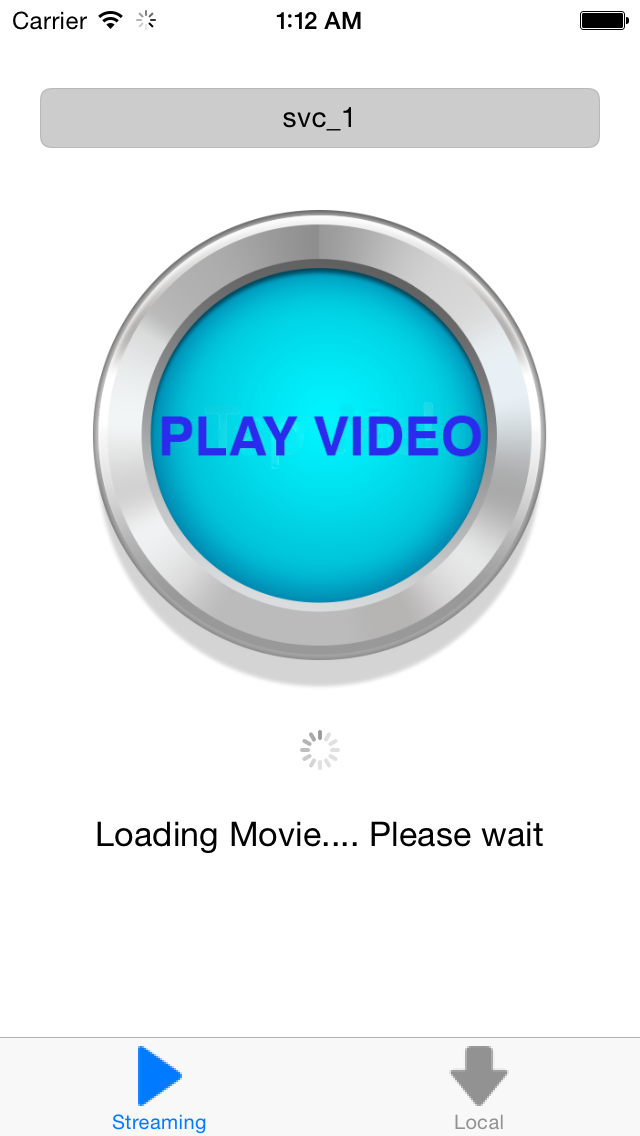
\includegraphics[width=0.3\textwidth]{./Images/ui_loading}} \qquad
	\subfigure[Play-out Session UI]{\label{fig:ui_playout}
		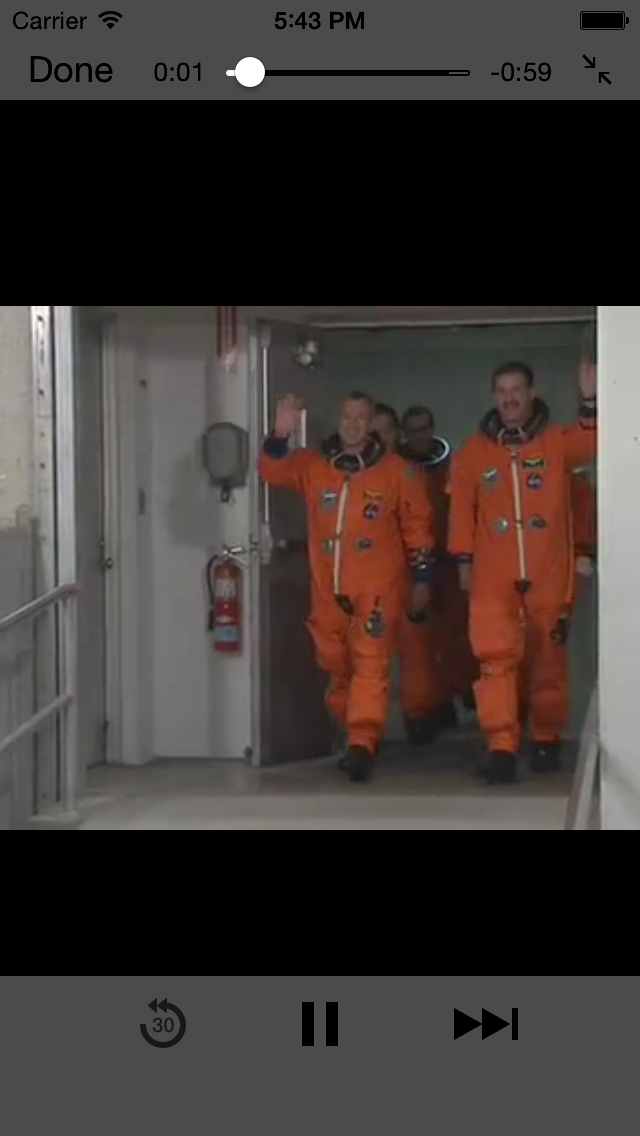
\includegraphics[width=0.3\textwidth]{./Images/ui_playout}}
	\caption{Complete User Interface}
	\label{fig:user_interface}
\end{figure}

Vestibulum ante ipsum primis in \ac{UI} faucibus orci luctus et ultrices posuere cubilia Curae; Nulla placerat aliquam wisi. Mauris viverra odio. Quisque fermentum pulvinar odio. Proin posuere est vitae ligula. Etiam euismod. Cras a eros.
% If Printing on DOUBLE SIDED pages, the second page should be white.
% Otherwise, comment the following command:
%\cleardoublepage
%
%Chapter 5
% #############################################################################
% This is Chapter 5
% !TEX root = ../main.tex
% #############################################################################
% Change the Name of the Chapter i the following line
\fancychapter{Results}
%%%%%%%%%%%%%%%%%%%%%%%%%%%%%%%%%%%%%%%%%%%%%%%%%%%%%%%%%%%%%%%%%%%%%%%%
%                                                                      %
%     File: Thesis_Results.tex                                         %
%     Tex Master: Thesis.tex                                           %
%                                                                      %
%     Author: Francisco Azeredo                                        %
%     Last modified :  2 Jul 2015                                      %
%                                                                      %
%%%%%%%%%%%%%%%%%%%%%%%%%%%%%%%%%%%%%%%%%%%%%%%%%%%%%%%%%%%%%%%%%%%%%%%%
\label{chap:results}

This chapter validates the architecture and approaches developed in Chapter~\ref{chap:systemarch} through comprehensive experiments on document extraction, schema-aware retrieval, and agentic versus naive \gls{RAG} systems. We evaluate retrieval effectiveness across multiple datasets and measure answer quality using diverse similarity metrics.

\section{Information Extraction and Document Structuring}

Multiple multimodal models were tested for information extraction: PrimaLayout and PubLayNet showed promise but were insufficiently trained and produced unpredictable results. Nougat, an OCR engine that preserves document hierarchy in Markdown format, was selected for cases where PDFs lack embedded text metadata.



\section{Metadata Extraction versus Naive RAG}
\subsection{LiHua-World Dataset}
\label{subsec:LiHua-World}
The knowledge graph experiment uses the \emph{LiHua-World} corpus from \cite{fan2025minirag}: a time-indexed set of short textual records organized into weekly folders (e.g., \path{week11/20260318_1510.txt}) and topical subfolders (e.g., \path{bakery_deliver/20260531.txt}). Each file contains concise, structured messages or notes about daily events (meetings, deliveries, fitness plans, chats, travel, garden updates), often implying participants and locations. This format provides:
\begin{itemize}
    \item \textbf{Temporal signals:} timestamps encoded in filenames (YYYYMMDD\_HHMM) and dates inside texts, enabling ordering and interval reasoning.
    \item \textbf{Multi-actor context:} recurring names across files (e.g., Li Hua, Wolfgang, Jennifer) support relationship extraction.
    \item \textbf{Domain variety:} community garden, bakery deliveries, fitness training, entertainment, and travel, which stress-test entity and relation typing.
\end{itemize}

\subsection{Knowledge Graph Ingestion Pipeline}

The corpus is processed through the metadata extraction framework by performing: (1) \textbf{Entity extraction:} using LLM-guided prompts to identify normalized entities (people, organizations, locations, events); (2) \textbf{Relation extraction:} inferring semantic relationships between entities based on embedding proximity; (3) \textbf{Object creation:} creating  Weaviate objects for extracted entities with cross-references; (4) \textbf{Vectorization}:embedding textual properties for hybrid retrieval.


In this setup, answers were generated using sentence embedding model All-MiniLM-L6-v2 for retrieval and the local LLM Qwen2M for generation. The benchmark dataset consisted of 628 questions categorized as: (1) \textbf{Single}—direct factoid questions that can be answered from a single evidence source; (2) \textbf{Multi}—questions requiring multi-hop reasoning and/or temporal or causal understanding; (3) \textbf{Null}—questions with insufficient evidence.

The experiment compares knowledge-graph–aware retrieval (Mini and Light) against a naive baseline.
Figure~\ref{fig:Lihua-World} presents the results across all metrics.
\begin{figure}[H]
    \centering
    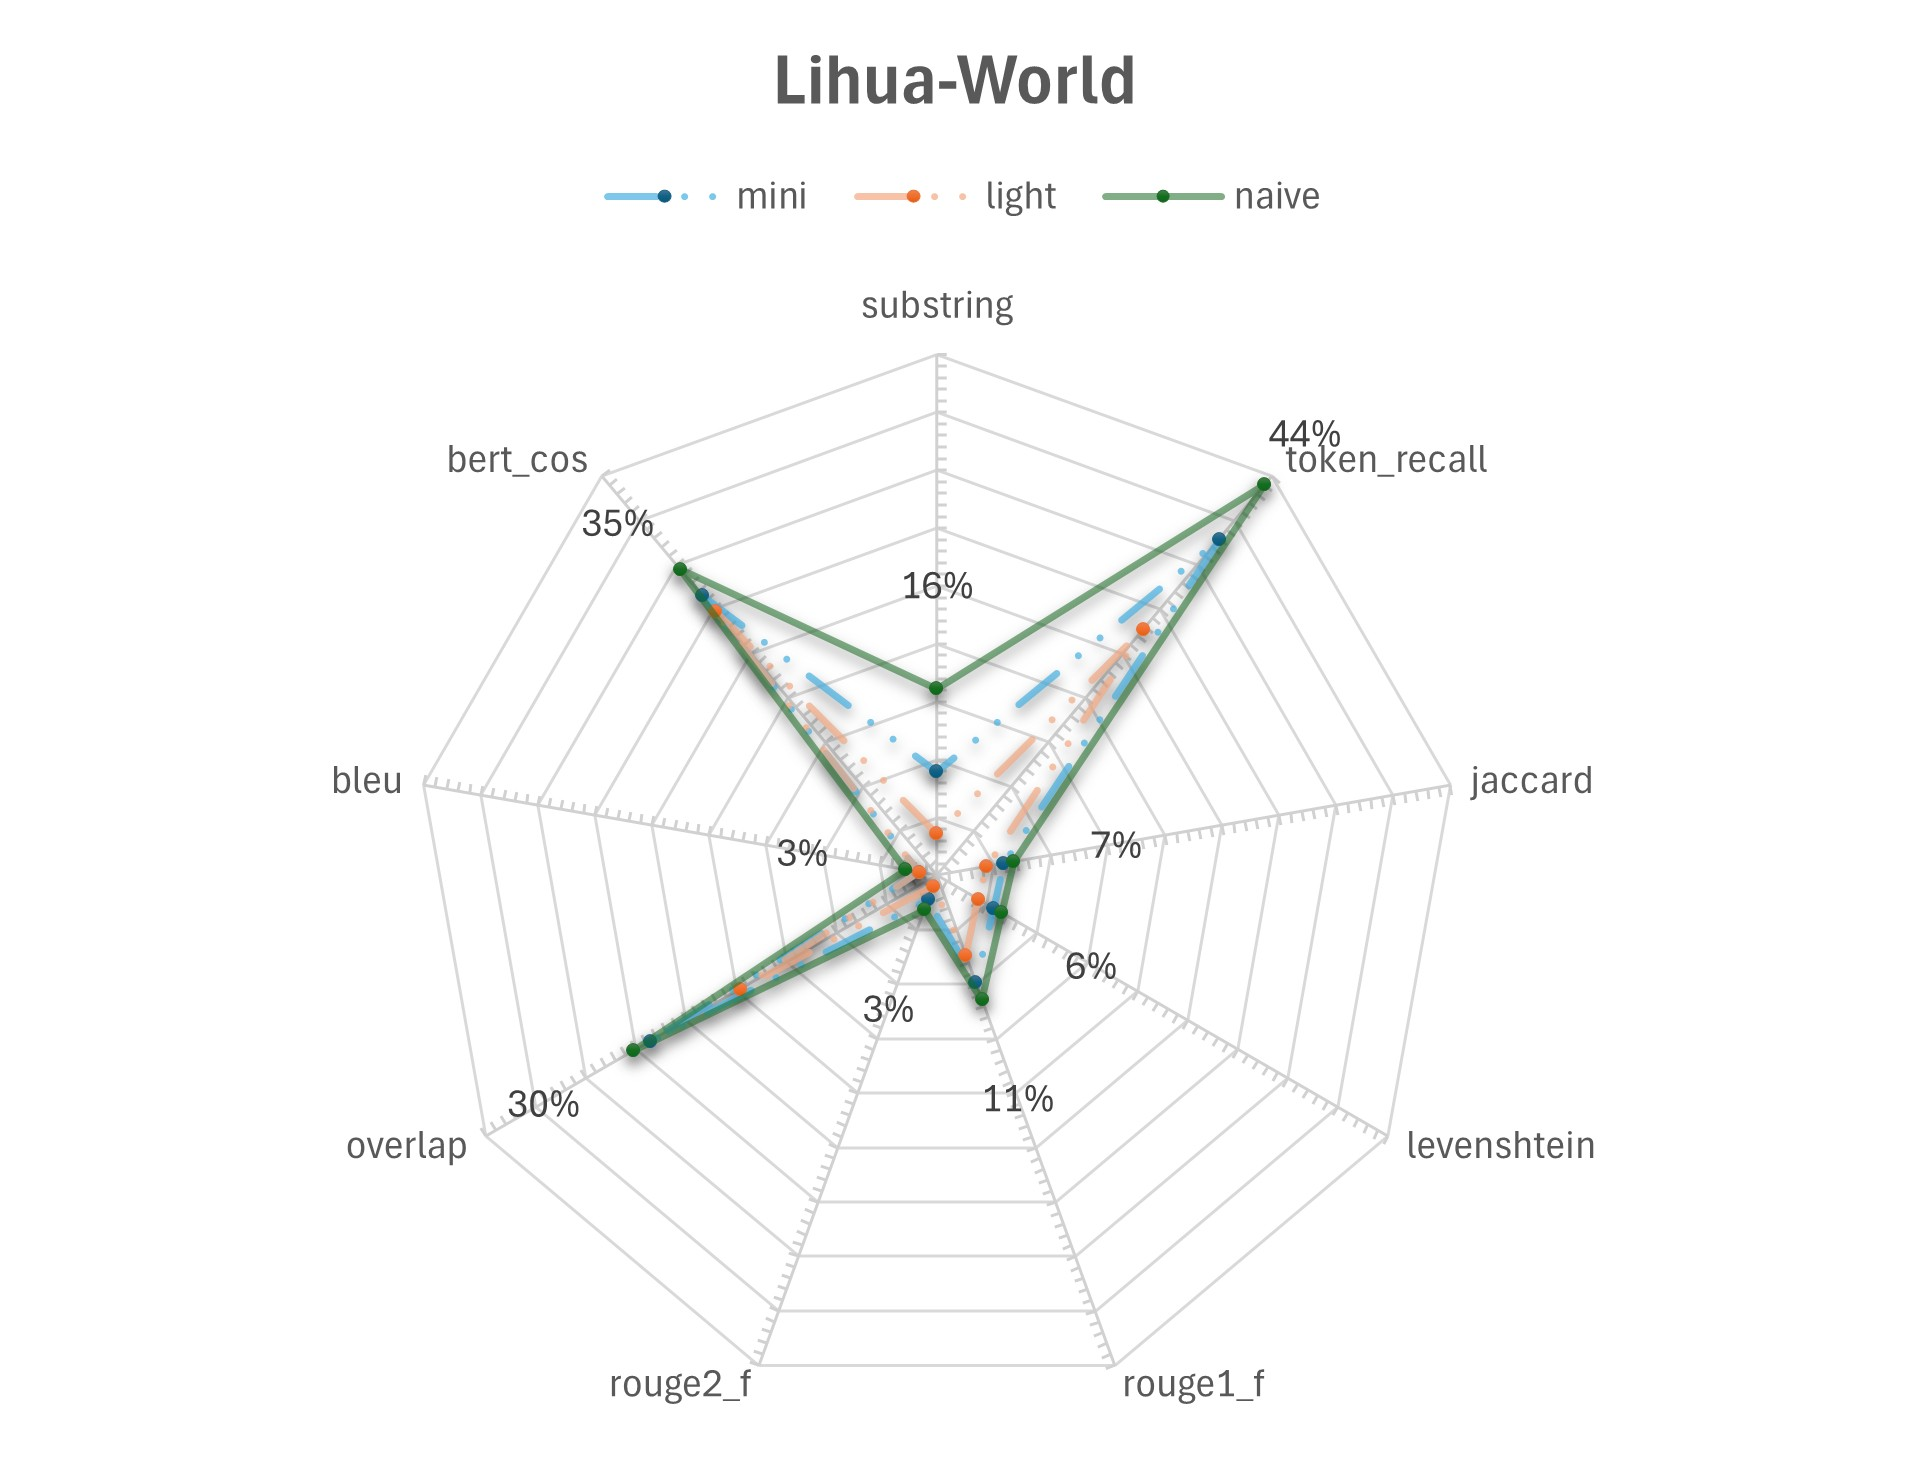
\includegraphics[width=1\linewidth]{Figures/Lihua-World.jpg}
    \caption{3 query types tested. With qwen2.5 as the \gls{LLM} and all-MiniLM-L6-v2 as embedding model}
    \label{fig:Lihua-World}
\end{figure}
Among the metrics, \textbf{Token Recall} achieved the highest score (44\%), and is the most relevant for this type of QA dataset.

\footnote{Note on metrics The full definitions and motivations for the evaluation metrics are provided in previous section \ref{sec:text-similarity-metrics}. Here we briefly reference the same set—lexical (Token Recall, Jaccard, Overlap), structural (Levenshtein, ROUGE, BLEU), and semantic (\gls{BERT} cosine)—and focus on interpreting the results in this experiment.}

\subsection{Semantic Similarity}
	\textbf{\gls{BERT} cosine similarity} score was moderate (35\%). This is largely due to length imbalance between short gold answers (sometimes a single token) and longer generated responses: sentence-level embeddings such as \textit{all-MiniLM-L6-v2} capture global semantics, so single-token vs. full-sentence comparisons tend to yield low cosine values.

\subsection{Lexical Accuracy}
	\textbf{Token Recall} (44\%) confirms that gold tokens are often present in predictions. The \textbf{Overlap Coefficient} (30\%) is comparatively robust to length differences, since it does not penalize extra tokens. In contrast, \textbf{Jaccard} (7\%) performs poorly when generated answers are longer, as the inflated union suppresses the overlap proportion—even for partially correct outputs.

\subsection{Structural Similarity}
	\textbf{Levenshtein} (6\%) provides a weak signal under large length differences. \textbf{ROUGE-1 F1} (11\%) and \textbf{ROUGE-2 F1} (3\%) partly mitigate this by balancing precision and recall over n-grams, although longer responses containing irrelevant tokens reduce precision. ROUGE-2 is particularly low because short gold answers rarely contain bigrams. Finally, \textbf{BLEU} (3\%)—originally designed for machine translation—over-penalizes deviations and brevity mismatches in this context, making it unsuitable for this task.

\subsection{Summary}
This experiment implemented an automated approach constructing a knowledge graph. The goal was to enable retrieval that leverages explicit entity relationships and organizational context rather than relying solely on surface-level text.

However, the results show that the current automatic knowledge graph construction fails to reliably produce a strong semantic structure for retrieval. In practice, direct embedding-based indexing using sentence transformers remains significantly faster, cheaper, and more effective for retrieval tasks, consistently outperforming the knowledge graph approach in this setup.

\textbf{Limitation acknowledgment:} It is important to note that this evaluation used \textbf{Qwen2.5}—a relatively small, locally-run language model—for knowledge graph construction (entity extraction, relation extraction, and summarization). The modest performance observed may therefore reflect the limitations of this specific model rather than the knowledge graph approach itself. Evaluating KG construction with stronger models (e.g., GPT-5 or similar) was beyond the scope and budget of this thesis, but would likely yield substantial improvements in both graph quality and downstream retrieval accuracy.

Profiling and structuring text with an LLM is also considerably more computationally expensive: each 200-token chunk is processed through a few-shot prompt (with many input tokens), up to three times, followed by an additional pass for entity merging and summarization. This makes large-scale knowledge graph construction costly. While using a heavier LLM could improve the quality of the knowledge graph and its retrieval performance, the resource requirements and latency increase substantially.

In summary, while knowledge graphs offer richer structure representations and could become more competitive with stronger \glspl{LLM}, current embedding models provide a more scalable and efficient solution for semantic retrieval. Future work should revisit knowledge graph approaches with more capable models, as the cost of \glspl{LLM} decreases and their capabilities improve.

\section{Naive \gls{RAG} versus \gls{ARAG} on Company Information}
\label{sec:expNaiveVsAgenticRAG}
This experiment aims to evaluate the effectiveness of an agentic retrieval-augmented generation (\gls{RAG}) approach compared to a naive \gls{RAG} baseline for answering context-specific questions about company information. The goal is to determine whether an agent capable of planning and reasoning over retrieved documents can provide more accurate and relevant answers than a straightforward retrieval and generation pipeline.

For this experiment, a synthetic company QA dataset was created in two automated stages:
\begin{enumerate}
        \item \textbf{Document Generation:} We synthesized 1{,}000 realistic administrative documents using  \gls{GPT}-5 via the OpenAI API. For each document, a classifiable node was sampled from a hierarchical public-sector classification (e.g., legislation, planning, HR, finance, justice, health, education) and prompted the model with the node’s description, notes, and index terms—while explicitly instructing it not to reveal the class name, both to preserve confidentiality when transmitting prompts to external APIs and to avoid label leakage. This produced a diverse set of plausible, well-structured administrative files spanning distinct legal and organizational contexts. This cost was approximately 2.50 dollars.
        \item \textbf{QA Pair Generation:} \label{subsec:qa-generation} Next, for a random subset of these documents, a second generative model (also \gls{GPT}-5) was employedto create question-answer pairs. The model was prompted with the full content of each document and instructed to generate a specific, contextually relevant question that could only be answered by reading that document, along with a precise answer based solely on its content. This ensures that each QA pair is tightly coupled to a single file and cannot be answered from general knowledge or other documents. The cost of generating 300 such QA pairs was approximately 0.85 dollars.
\end{enumerate}

This process produces the \gls{QA} benchmark used to evaluate thedeveloped \gls{RAG} systems, where each question can only be answerable by retrieving the correct company file and reasoning over its content. The dataset is well-suited for evaluating (\gls{RAG}) systems, as it necessitates both accurate retrieval and grounded answer generation.

\subsection{Vector Database Setup}
The vector database employed in this work is Weaviate. It is populated with 1000 synthetic company documents created earlier (see Section~\ref{sec:expNaiveVsAgenticRAG}) and indexed using \textit{sentence-transformers/all-MiniLM-L6-v2} embeddings. The schema is straightforward: a single class, \textit{Ficheiro} (file), with properties \texttt{text} and \texttt{file\_path}. Each document is stored as one object, with \texttt{text} vectorized (named vector \texttt{text\_vector}) to support semantic search; \texttt{file\_path} stores the document source for grounding answers. This index is employed by both the naive and agentic systems in the following experiments.

\subsection{Naive RAG and CoT Baselines}
\label{sec:naive-rag-and-cot-baseline}
The naive baseline retrieved top-ranked passages from Weaviate and produced an answer; the CoT variant used the same retrieval with a concise step-by-step hint.
For each question in the \gls{QA} dataset (generated in \ref{subsec:qa-generation}), the naive pipeline executes:
\begin{enumerate}
    \item Run a hybrid search in Weaviate (\(\alpha = 0.7\)) over \texttt{text\_vector} with the question to retrieve the top-$k$ objects containing \texttt{text} and \texttt{file\_path}.
    \item Generate a concise answer grounded in the retrieved content.
\end{enumerate}

At a high level, the naive pipeline performs a single retrieve-and-generate pass over hybrid search results in Portuguese. Variants with \texttt{qwen2.5} were tested to pick a cost-effective baseline, then the best was re-run with ChatGPT-5 to estimate an upper bound on quality. See Algorithm~\ref{alg:naive-weaviate-hybrid} (Appendix~B) for details.
The results are presented in Figure~\ref{fig:weaviate_test}.
This serves as a control: it is simpler to implement and does not require a large model for planning.
\begin{figure}
    \centering
    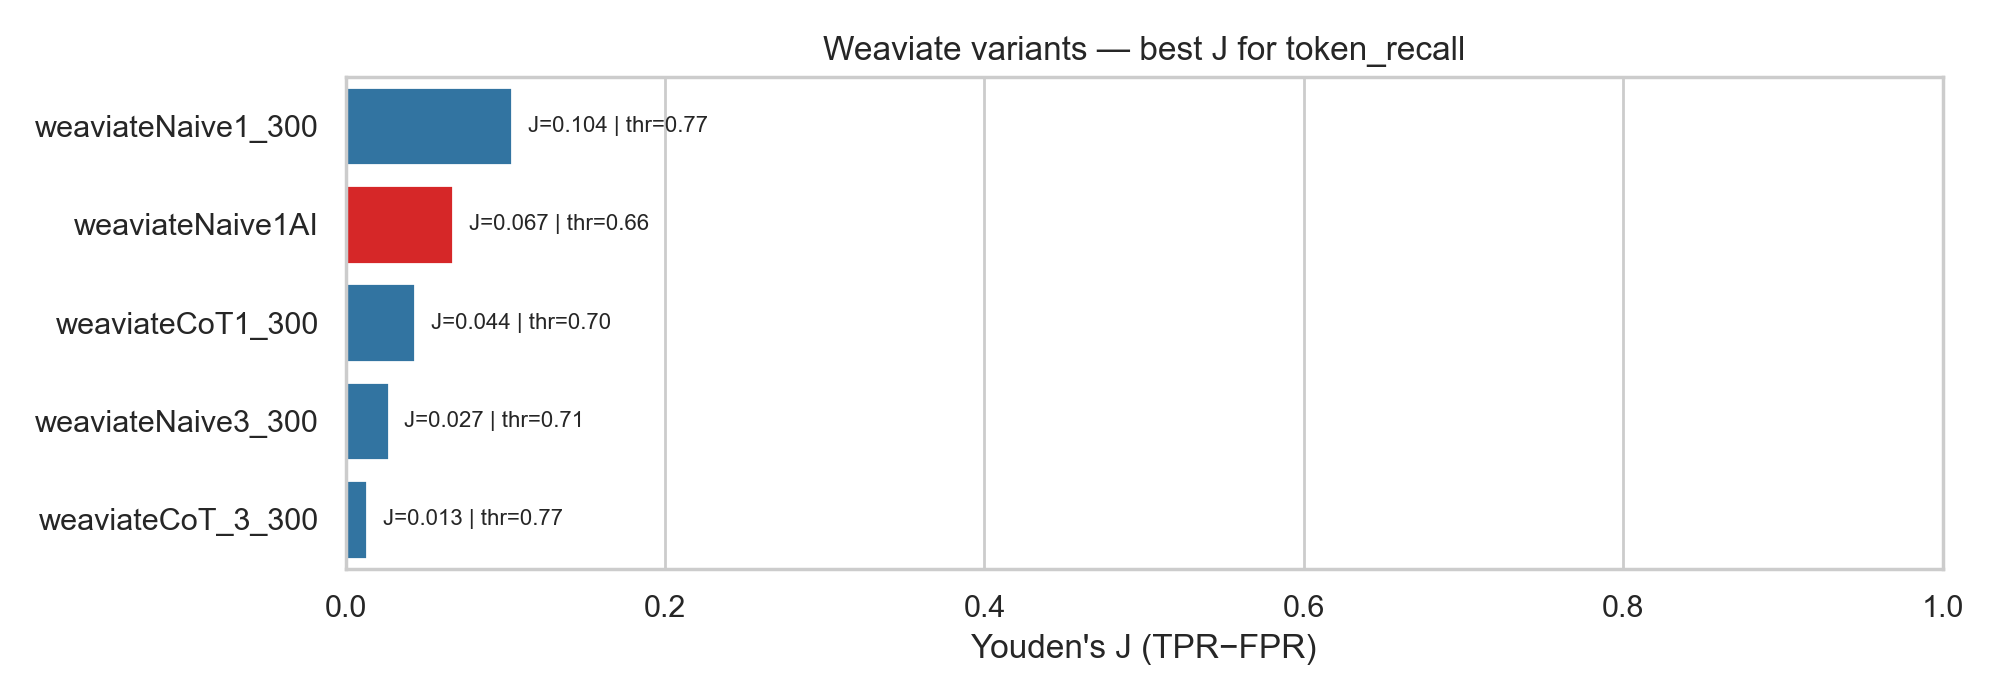
\includegraphics[width=1\linewidth]{Figures/10_weaviate_best_j_token_recall.png}
    \caption{Youden's J statistic for qualifying best naive \gls{RAG} variant. With qwen2.5m as the \gls{LLM} and all-MiniLM-L6-v2 as embedding model. And a chatgpt5 variant using best top-$k$ and prompt parameters.(k=4, prompt=naive)}
    \label{fig:weaviate_test}
\end{figure}
\subsection{Agentic RAG Setup}
\label{sec:agentic-test}

To set up the test, a \textbf{ReAct} agent was developed and connected to a Weaviate vector database via \gls{MCP} developed in this thesis~\ref{sec:weaviate-mcp-server}. Following initial trials with a local model (\texttt{qwen2.5m}) that exhibited frequent context drift—diverging from the question and producing extractive outputs—reinforcing the need for a larger context window, \textbf{ChatGPT-5} was used for planning and generation, since larger model is required to maintain multi-step reasoning within its context window.

\subsection{Agent Workflow}
For each question in the \gls{QA} dataset (generated in \ref{subsec:qa-generation}), the agent follows a ReAct loop:
\begin{enumerate}
\item \textbf{Plan:} Sketch a brief strategy to find the answer.
\item \textbf{Retrieve:} Fetch the most relevant documents.
\item \textbf{Observe \& Reflect:} Inspect the evidence and, if needed, refine the plan and retrieval.
\item \textbf{Answer:} Produce a concise response grounded in the retrieved content.
\end{enumerate}

Across \textbf{300} questions, the agent sometimes required up to \textbf{20} \gls{LLM} calls per query, with a total run cost of approximately \textbf{\$14}. While reasoning improves answer quality, it significantly increases latency and cost compared to naive \gls{RAG}.

The cost-quality trade-off can be expressed as: achieving 60.4\% retrieval rate via agentic \gls{RAG} costs approximately \textbf{\$0.047 per question}, compared to \textbf{\$0.0017} for naive \gls{RAG} at 13.8\% retrieval. This \textbf{27.6x cost increase} yields a \textbf{4.4x improvement in retrieval accuracy}, representing a favorable trade-off for scenarios where accuracy is prioritized over cost.

\section{Evaluation of Quality Metrics}
\label{sec:metric-evaluation-quality}
To evaluate answer quality, the same metrics as in the previous experiment (Section~\ref{sec:expNaiveVsAgenticRAG}) are applied. Theanalysis extends further under the hypothesis that an answer can only be correct if thecorresponding souce is correctly retrieved. This is assessed by determining the metric threshold that best separates correct from incorrect answers—i.g., the threshold that most closely aligns with successeful source retrieval. The optimal threshold is identified by maximizing Youden's J statistic, defined as the difference between true positive rate (TPR) and false positive rate (FPR).
\begin{figure}[H]
    \centering
    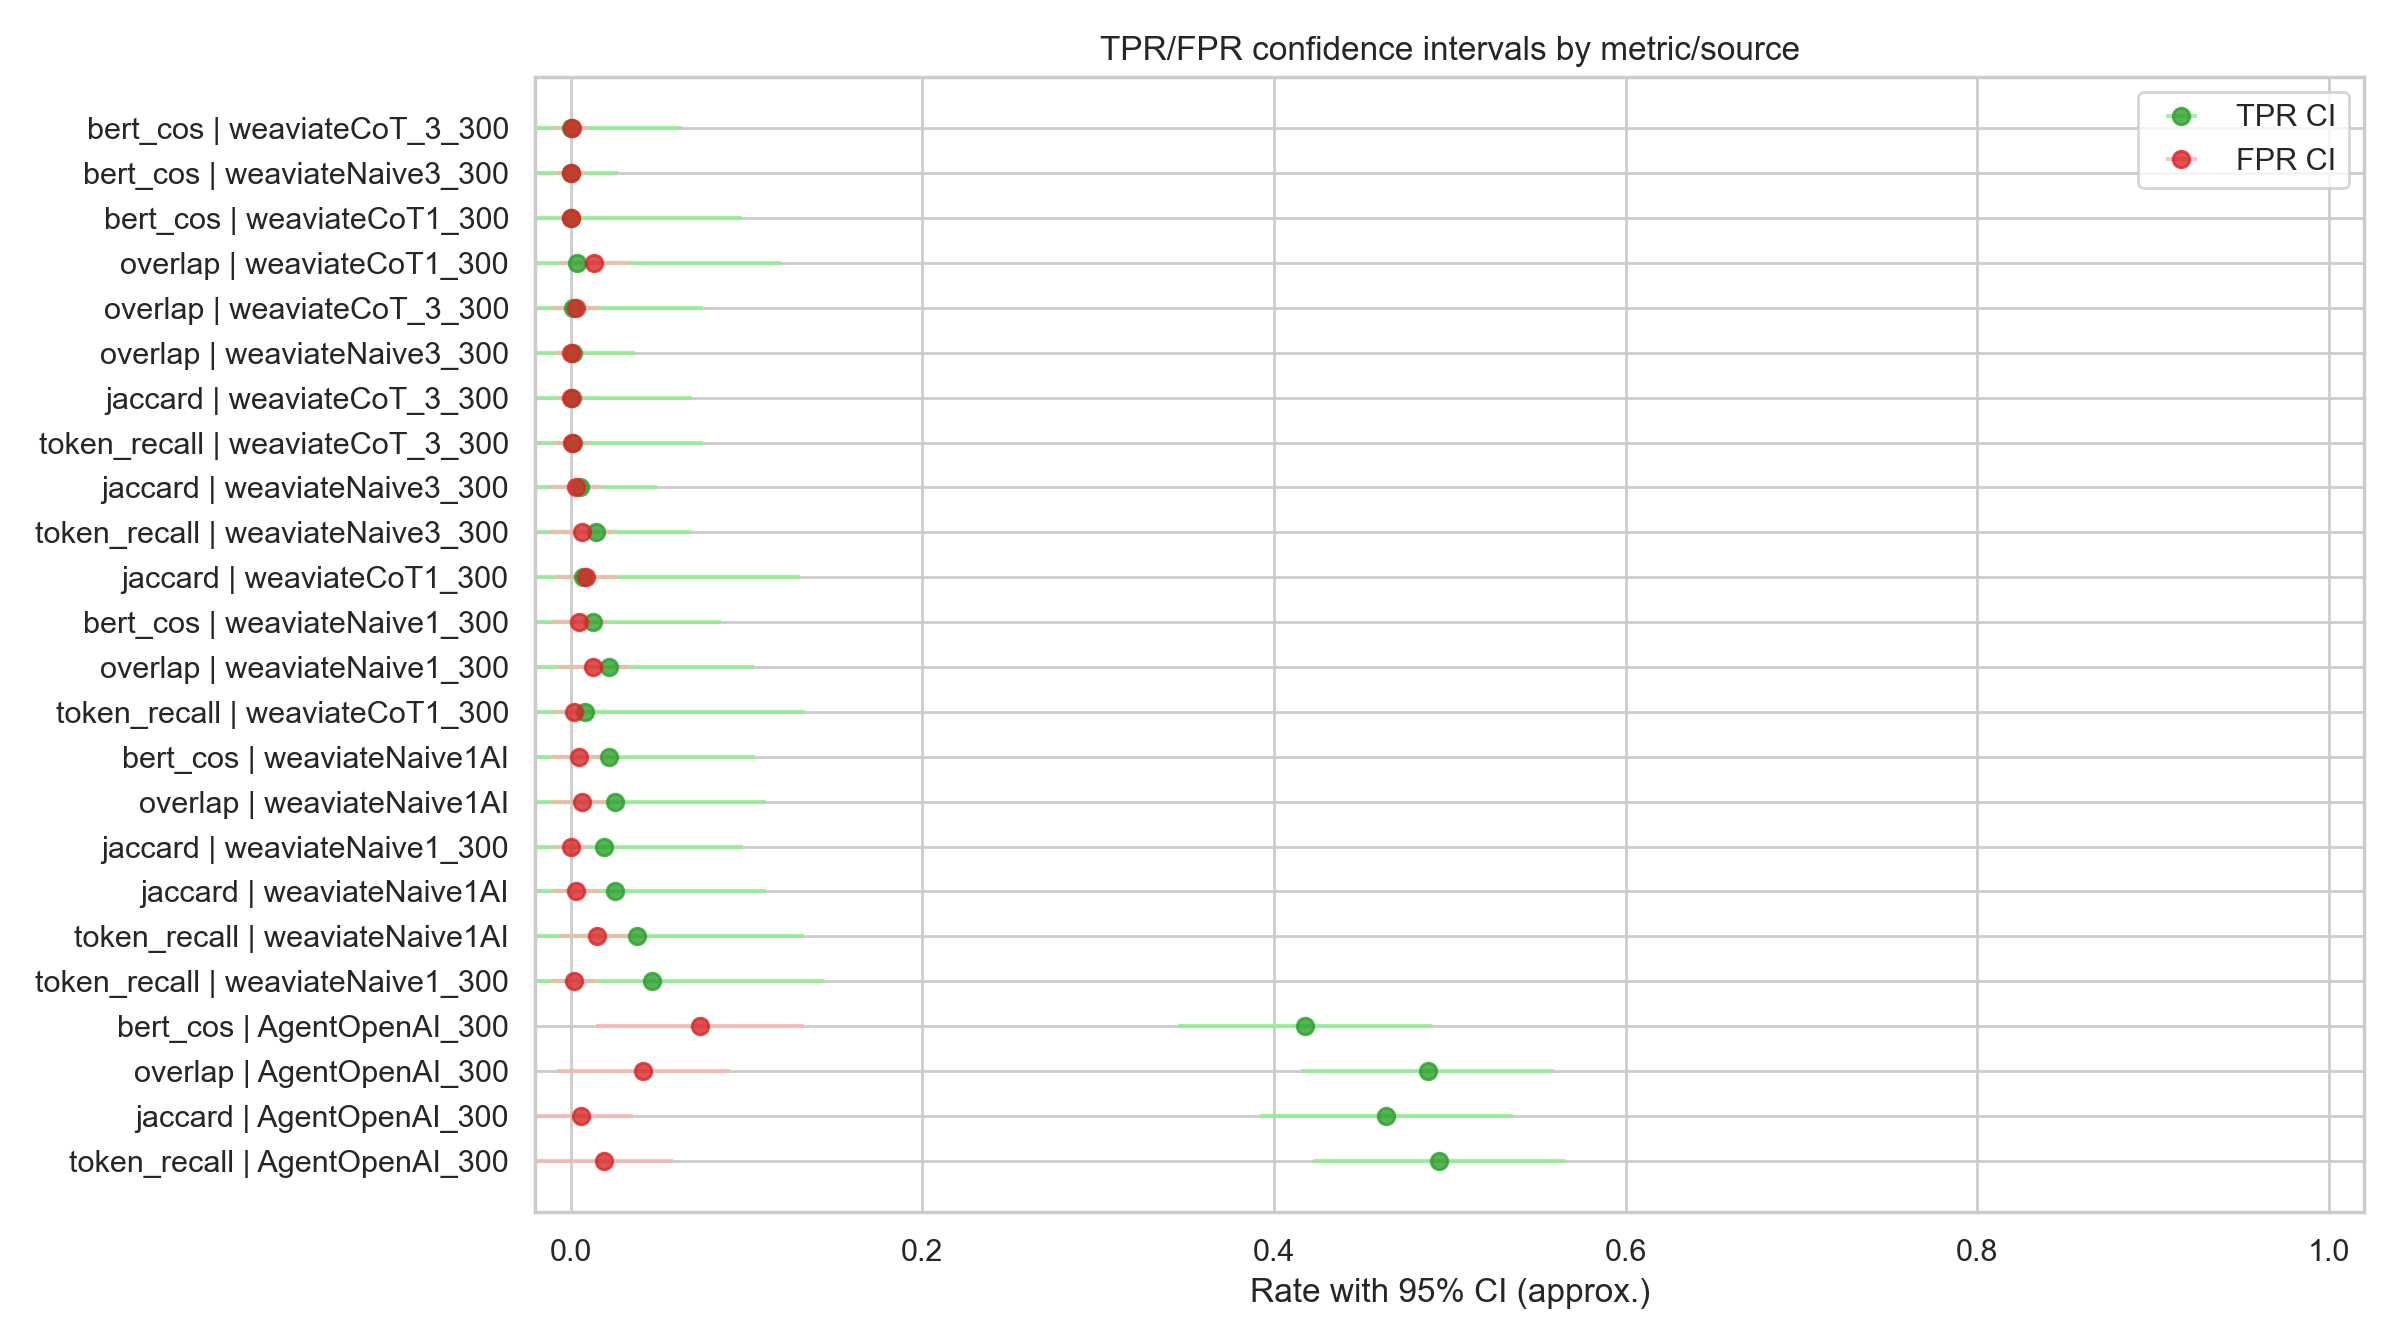
\includegraphics[width=1\linewidth]{Figures/06_tpr_fpr_confidence_intervals.png}
    \caption{confidence intervals for TPR and FPR per metric, for all source benchmark results, using the threshold that maximizes Youden's J statistic.}\label{fig:confidence-intervals}
\end{figure}

From the TPR and FPR confidence intervals (Figure~\ref{fig:confidence-intervals}), it can be observed that results obtained from the agentic RAG system have much better quality than the naive RAG system across all metrics. This indicates that the most reliable benchmark for determining thresholds using Youden's J statistic is the agentic RAG system. One contributing factor is its more balanced behavior on missed and successful retrievals. As seen from the document retrieved percentages shown in Table~\ref{tab:doc-retrieved-by-source}, the agentic RAG system substantially outperforms naive baselines: it correctly retrieves documents 60.4\% of the time, compared to 13.8\%–22.5\% for naive approaches and 5.7\%–9.4\% for chain-of-thought variants. This substantial improvement reflects the agent'sreasoning and planning capabilities, whereas the naive RAG system performs a single hybrid search.

\begin{table}[htbp]
    \centering
    \begin{tabular}{l c}
        \hline
        Source file & Correct document retrieved \\
        \hline
    AgentOpenAI\_300 & 60.4\% \\
    weaviateNaive3\_300 & 22.5\% \\
    weaviateNaive1\_300 & 13.8\% \\
    weaviateNaive1AI & 13.4\% \\
    weaviateCoT\_3\_300 & 9.4\% \\
    weaviateCoT1\_300 & 5.7\% \\
        \hline
    \end{tabular}
    \caption{Document retrieved percentage by source file}\label{tab:doc-retrieved-by-source}
\end{table}

\begin{table}[htbp]
  \centering
  \begin{tabular}{l c c c c}
    \hline
    Metric & Threshold & TPR & FPR & J \\
    \hline
    token\_recall & 0.67 & 56.7\% & 4.4\%  & 52.3\% \\
    jaccard       & 0.26 & 53.7\% & 2.0\%  & 51.7\% \\
    rouge1\_f     & 0.40 & 52.3\% & 2.7\%  & 49.7\% \\
    overlap       & 0.56 & 56.0\% & 7.7\%  & 48.3\% \\
    bleu          & 0.37 & 39.3\% & 1.3\%  & 37.9\% \\
    bert\_cos     & 0.71 & 49.0\% & 12.1\% & 36.9\% \\
    \hline
  \end{tabular}
    \caption{Best thresholds by metric (max True--False pass-rate difference) for File: AgentOpenAI\_300}\label{tab:agentopenai300-best-thresholds}
\end{table}


\subsection{Overall Metric Results}
Based on the previous subsection, the analysis indicates that the optimal metric thresholds (according to Youden's J statistic) are delivered from the agentic RAG system; these thresholds from table \ref{tab:agentopenai300-best-thresholds} are subsequently used to classify answers as correct or incorrect across benchmarks. The analysis is also narrowed to the best naive RAG variant (weaviateNaive1\_300), using qwen2.5 and OpenAI models, and the agentic RAG system (AgentOpenAI\_300). The results are presented in Figure~\ref{fig:median-metric} and Table~\ref{tab:gain-loss-reference-median}. The median metric scores are also presented for reference.
\begin{figure}
    \centering
    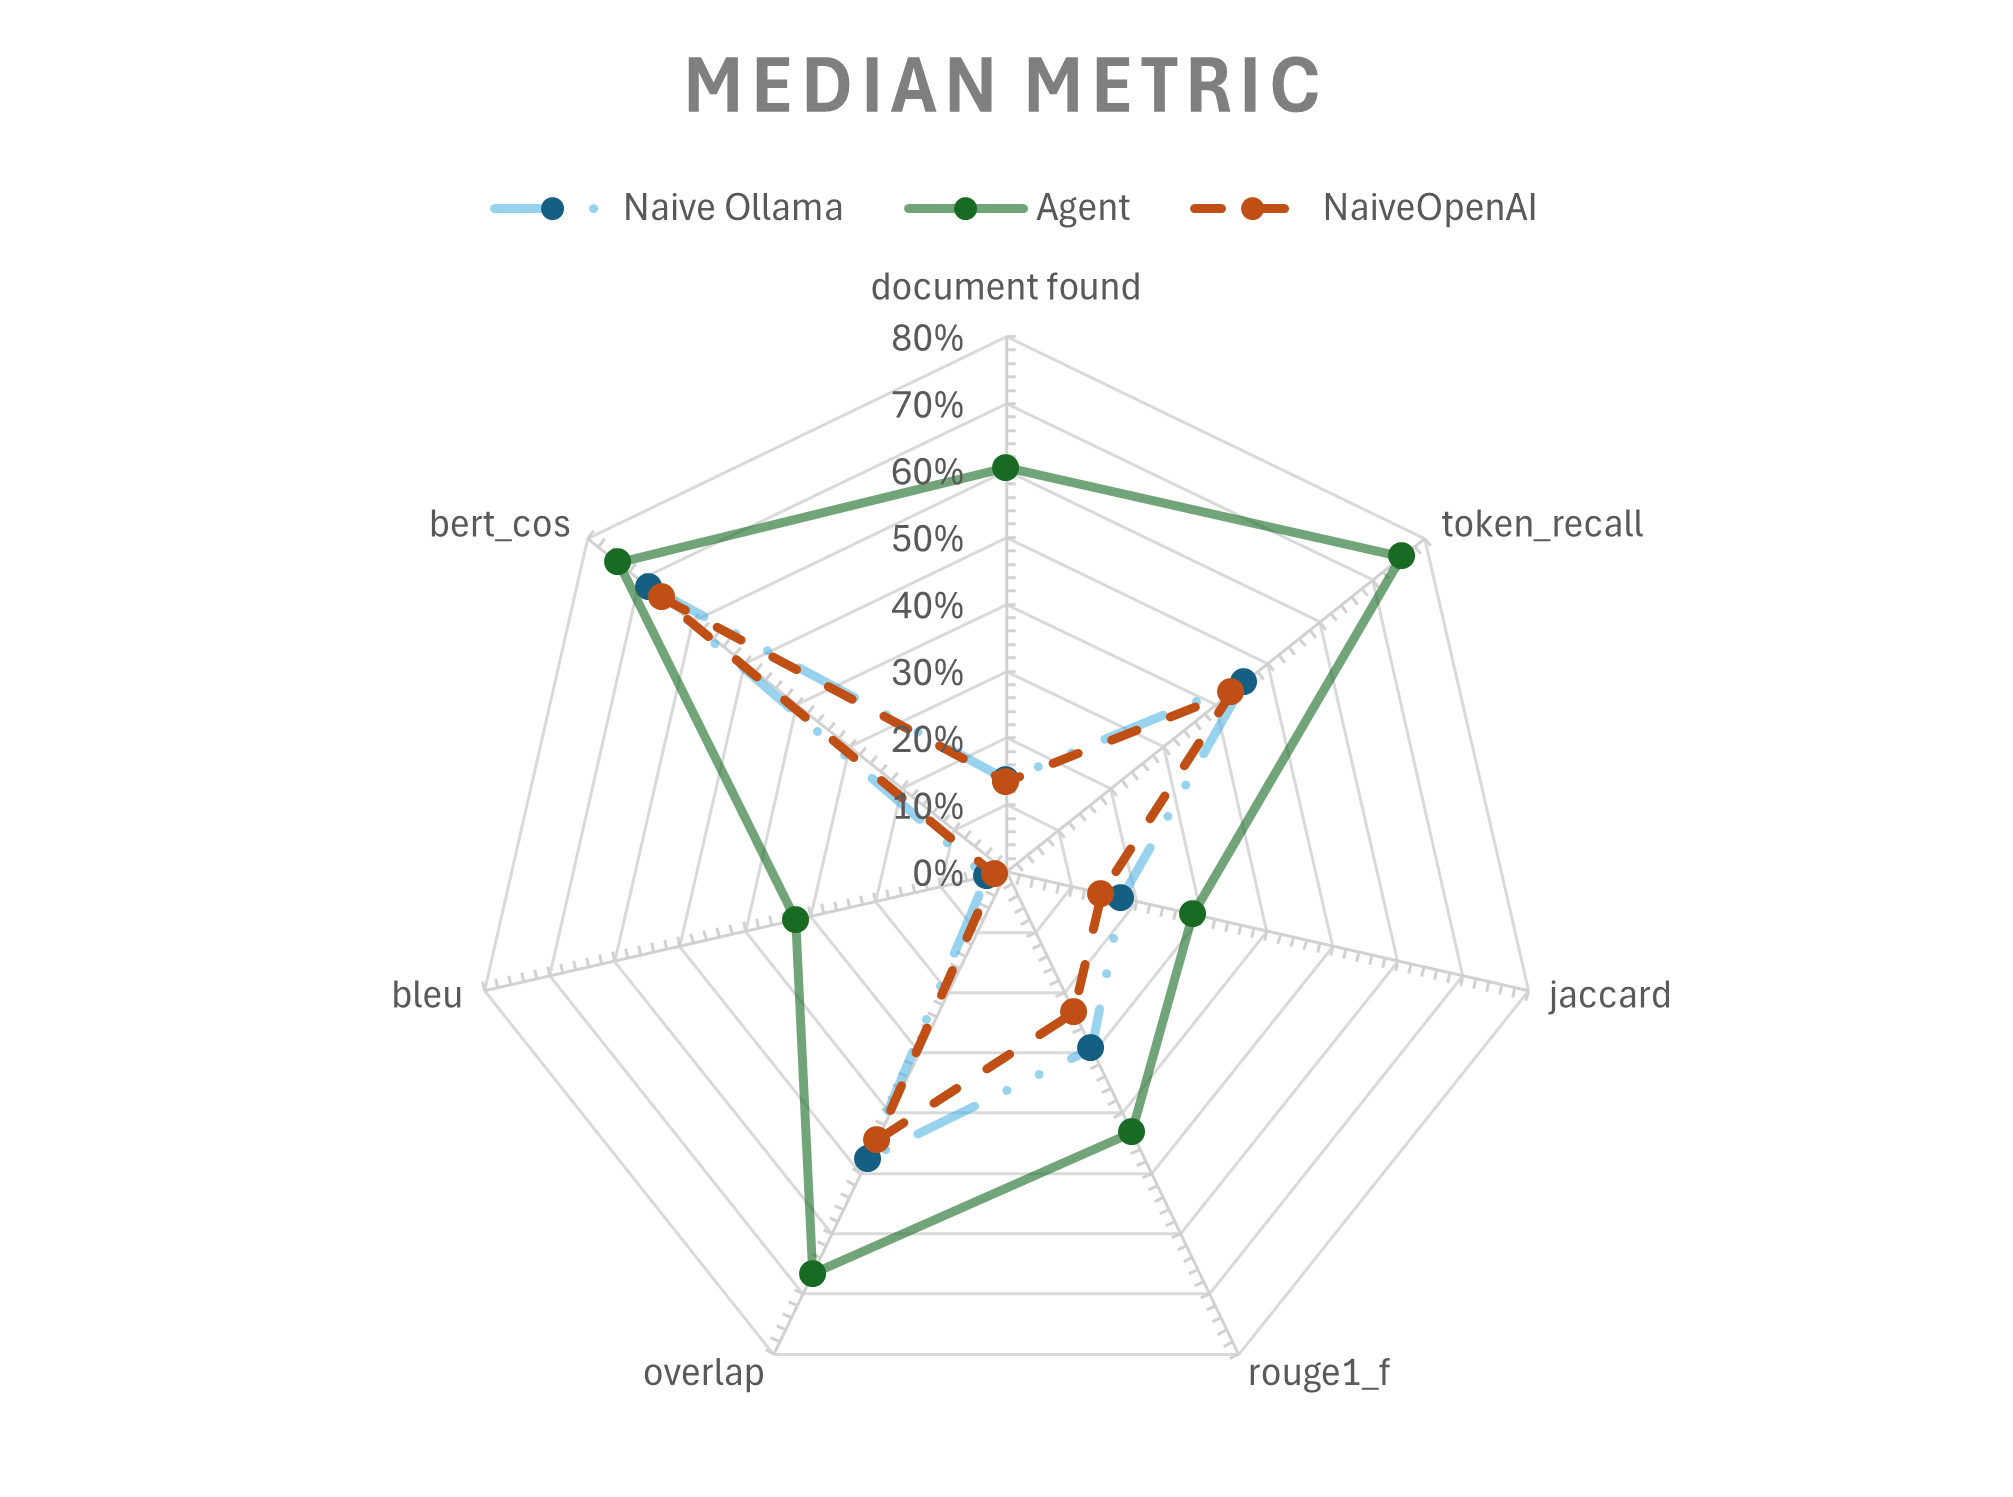
\includegraphics[width=0.75\linewidth]{Figures/Median Metric.png}
    \caption{Median Metric Scores}\label{fig:median-metric}
\end{figure}
According to Table~\ref{tab:agentopenai300-best-thresholds}, the metrics ranked by Youden's J statistic are: \textbf{Token Recall}, \textbf{Jaccard}, \textbf{ROUGE-1 F1}, \textbf{Overlap}, \textbf{BLEU}, and \textbf{\gls{BERT} cosine}. This ranking shows which thresholds are most effective for distinguishing correct from incorrect answers in this dataset. Token Recall attains the highest Youden's J value (52.3\%) because questions are specific, and correctness depends on including the correct content words, while surface fluency or paraphrase similarity is less critical. The -15\% trade-off observed in Table~\ref{tab:gain-loss-reference-median} reflects a deliberate threshold calibration: by optimizing for precision-oriented metrics (Jaccard, ROUGE-1), Token Recall is slightly reduced to prevent false positives, yielding a better overall classification balance. Conversely, \gls{BERT} cosine—which emphasizes sentence-level semantic similarity—performs worst here because many gold answers are short and exactness is essesntial. Jaccard performs well because it rewards coverage of relevant tokens relative to the union, serving as a useful proxy for answer completeness.

\begin{table}[htbp]
    \centering
    \begin{tabular}{l r r r  r r r}
        \hline
        Approach &  token recall & jaccard & rouge1 & overlap & bleu & \gls{BERT} cosine \\
        \hline
        Agentic ReAct (\gls{GPT}-5) &  -15\% & 27\% & 12\% & -3\% & 8\% & -13\% \\
        Naive \gls{RAG} (\gls{GPT}-5) &  -31\% & -1\% & -9\% & -16\% & 1\% & -38\% \\
        Naive \gls{RAG} (Qwen2.5) &  -26\% & 5\% & -8\% & -9\% & -1\% & -30\% \\
        \hline
    \end{tabular}
    \caption{Numerical differences when using agentic reference thresholds (Youden-optimized)\ref{fig:Youden-metric} versus median-based \ref{fig:median-metric} thresholds for classifying answers (positive values indicate gains).}
    \label{tab:gain-loss-reference-median}
\end{table}

Applying the agentic reference thresholds yields clear gains for \textit{Agent OpenAI} on \textit{Jaccard} (+27\%), \textit{ROUGE-1} (+12\%), and \textit{BLEU} (+8\%), with a trade-off in \textit{Token Recall} (\textminus 15\%). \textit{\gls{BERT} cosine} declines (\textminus 13\%) are expected give the stricter, token-accuracy oriented thresholding. The naive baselines exhibit broad declines—particulary in \textit{Token Recall} and \textit{\gls{BERT} cosine}—indicating that thresholds calibrated on higher-quality, better-retrieved agentic outputs do not gerenalize well to weaker systems.
\begin{figure}
    \centering
    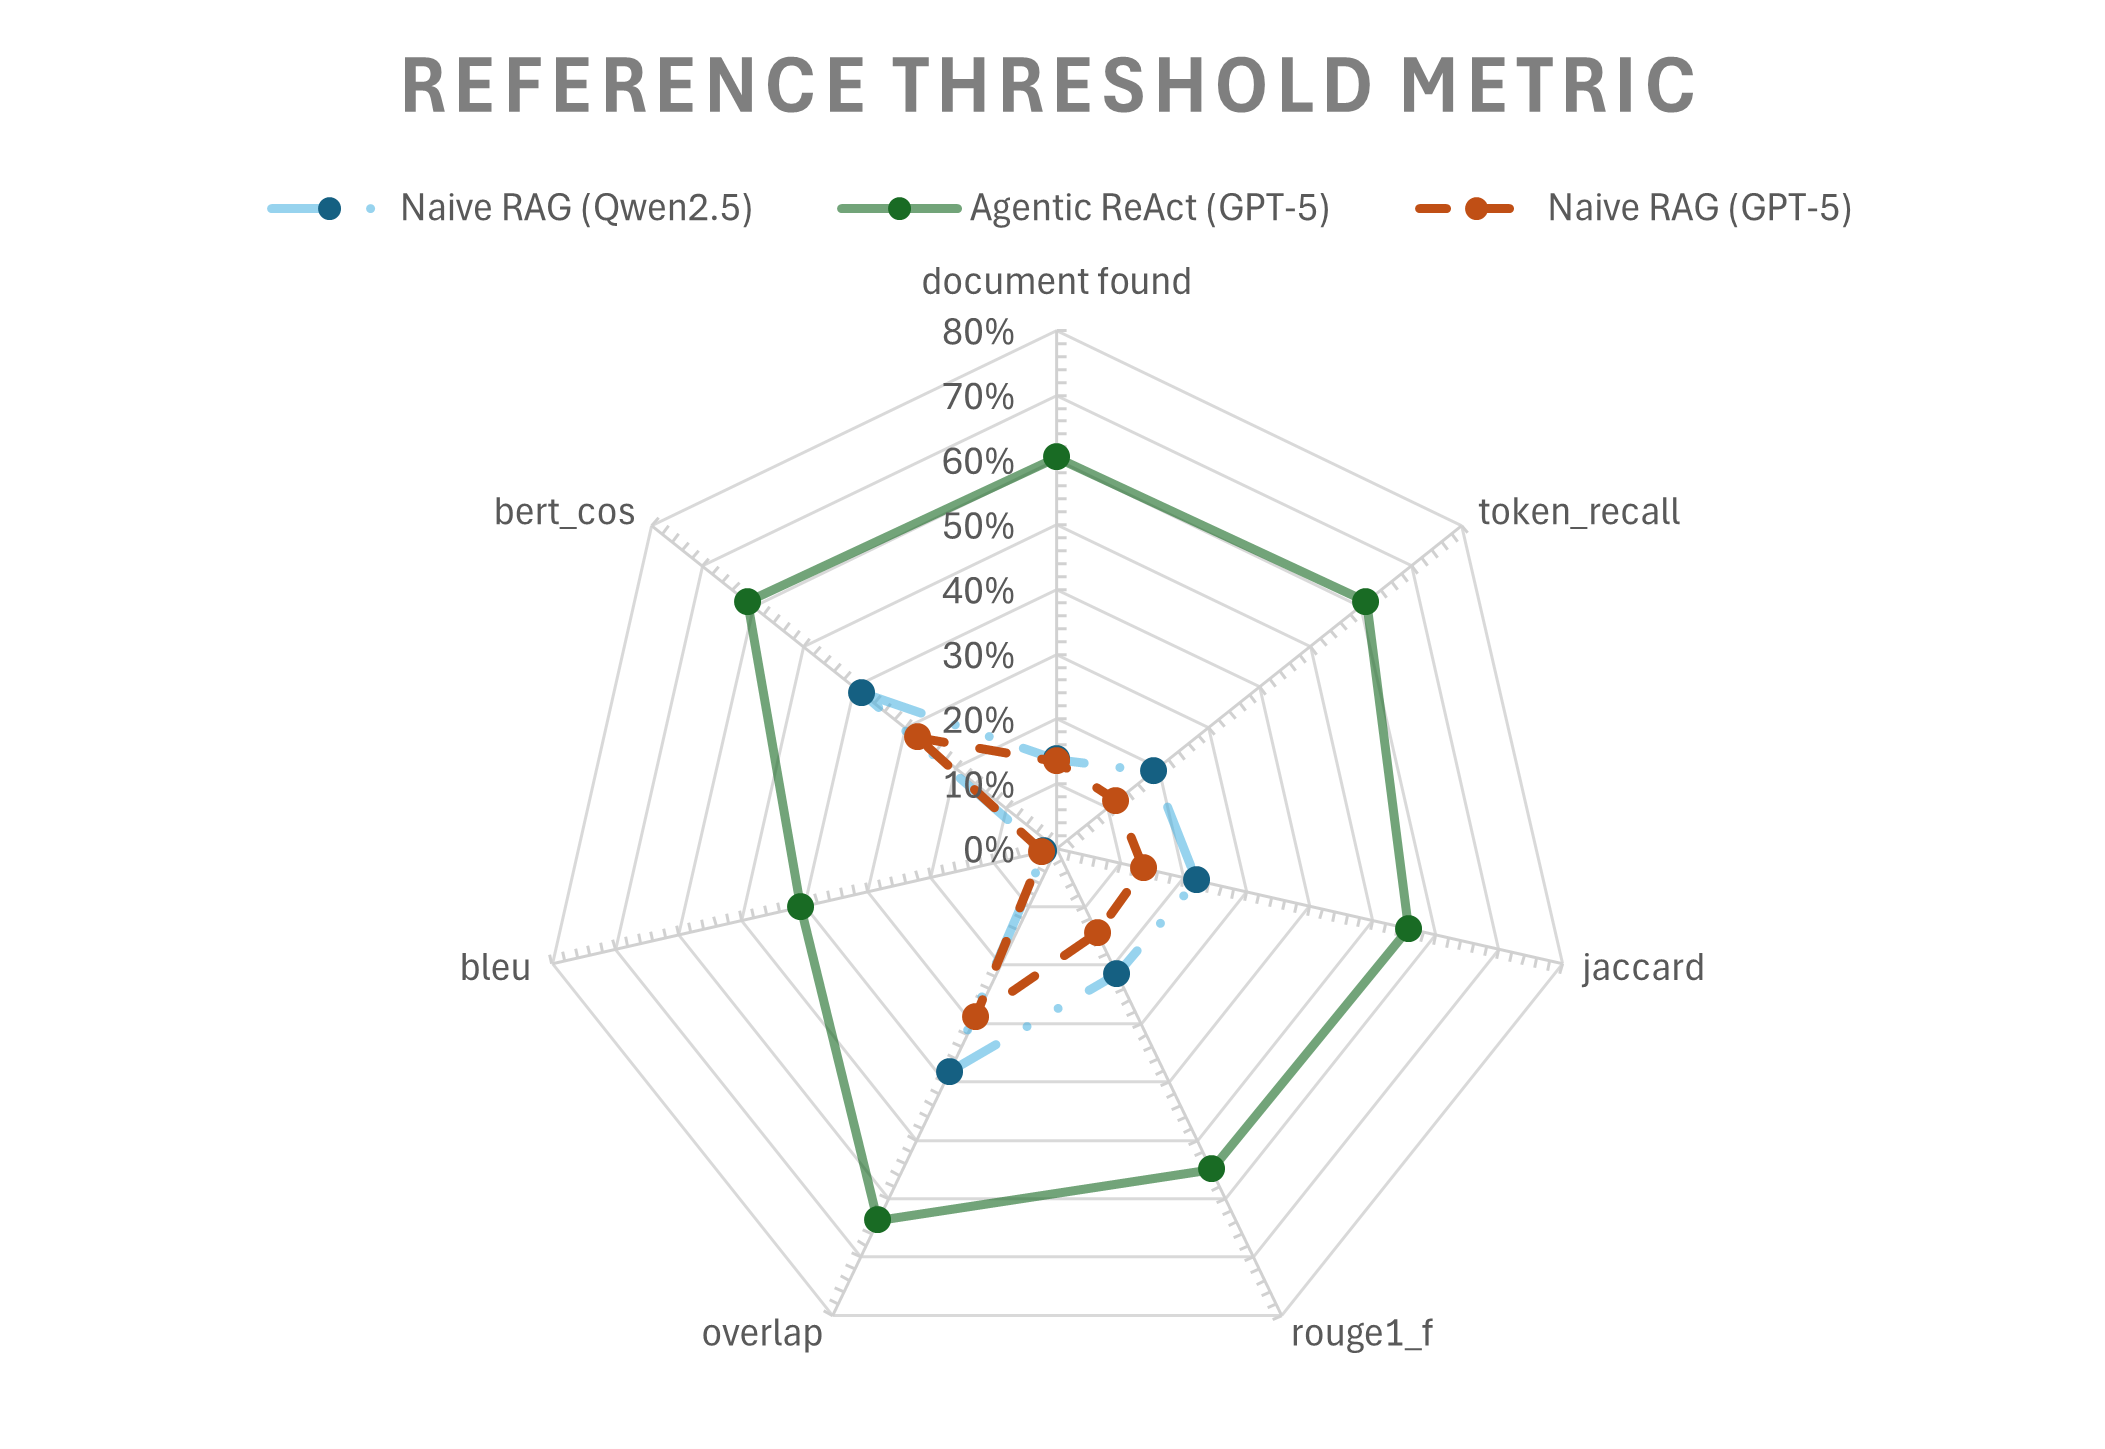
\includegraphics[width=0.75\linewidth]{Figures/Reference Threshold Metric.png}
    \caption{Agentic AI reference thresholds applied to all metrics of all important benchmarks}\label{fig:Youden-metric}
\end{figure}

Compared to the median-based thresholds, the agentic reference thresholds yield a more favorable profile for the \textit{Agent OpenAI} benchmark, boosting precision-oriented metrics (\textit{Jaccard}, \textit{ROUGE-1}, \textit{BLEU}) while sacrificing some recall (\textit{Token Recall}), while still maintaining a high score. This reflects the agent's ability to retrieve and synthesize relevant information more accurately, even if it occasionally omits less critical details. The naive baselines, however, do not benefit from this calibration, since their lower-quality outputs align less aligned well with the stricter criteria derived from the agentic system.

\begin{table}[htbp]
    \centering
    \begin{tabular}{l r r r r r r}
        \hline
        Approach & token recall & jaccard & rouge1f & overlap & bleu & \gls{BERT} cosine \\
        \hline
        Agentic ReAct (\gls{GPT}-5) & 61\% & 56\% & 55\% & 64\% & 41\% & 61\% \\
        Naive \gls{RAG} (\gls{GPT}-5) & 12\% & 14\% & 14\% & 29\% & 2\% & 28\% \\
        Naive \gls{RAG} (Qwen2.5) & 19\% & 22\% & 21\% & 38\% & 2\% & 39\% \\
        \hline
    \end{tabular}
    \caption{Share of answers passing Youden-optimized thresholds (Figure~\ref{fig:Youden-metric})}
    \label{tab:youden-metric-values}
\end{table}

Taken together with Figure~\ref{fig:Youden-metric}, these values show a pronounced separation between the agentic system and naive baselines under Youden-optimized criteria. The \textit{Agent OpenAI} workflow—plan, retrieve, observe/reflect, and answer—consistently classifies a much larger fraction of outputs as correct across metrics (e.g., 61\% Token Recall and 64\% Overlap), whereas naive pipelines lag substantially (e.g., Token Recall 12–19\%, Overlap 29–38\%). This demostrates the benefit of iterative reasoning and refinement over a single-pass naive RAG. This is also coupled by the fact that agentic RAG retrieves more documents correctly than the naive RAG system, as seen in Table~\ref{tab:doc-retrieved-by-source}.

\subsection{Cost and Latency Trade-offs}

Table~\ref{tab:naive-vs-agentic-tradeoffs} summarizes the cost and performance trade-offs between naive and agentic \gls{RAG} approaches. While naive \gls{RAG} is faster and cheaper (single retrieval + generation pass), agentic systems incur higher costs due to multiple reasoning and retrieval cycles. However, the significantly improved retrieval rate (60.4\% vs. 13.4\%–13.8\%) and answer quality justify this trade-off in mission-critical retrieval tasks.

\begin{table}[htbp]
    \centering
    \begin{tabular}{l r r r}
        \hline
        Approach & \gls{LLM} Calls/Query & Total Cost (300 Q) & Avg. Retrieval Rate \\
        \hline
        Naive \gls{RAG} (Qwen2.5) & 1--2 & 0 & 13.8\% \\
        Naive \gls{RAG} (\gls{GPT}-5) & 1--2 & \$5.07 & 13.4\% \\
        Agentic ReAct (\gls{GPT}-5) & 5--20 & \$18.35 & 60.4\% \\
        \hline
    \end{tabular}
    \caption{Comparative analysis of cost, latency, and retrieval effectiveness between naive and agentic \gls{RAG} approaches. Agentic systems require more \gls{LLM} calls but achieve substantially higher retrieval accuracy.}
    \label{tab:naive-vs-agentic-tradeoffs}
\end{table}

\section{Agentic Retrieval Across Multiple Collections}
\label{sec:agentic-retrieval-multiple}
In this experiment, the effectiveness of using multiple collections in Weaviate is evaluated and it is determined whether the agentic RAG system from Section~\ref{sec:agentic-test} can retrieve information distributed across multiple collections. The goal is to assess whether the agent can effectively navigate multiple data sources.

This is relevant in real-world scenarios where company information is distributed across separate databases or collections, each organized by department, project, or document type. For example, a media publisher may purchase content feeds from multiple providers. Each provider might expose its catalog through a Weaviate instance and sell API access rather than delivering raw data. With a successful agentic RAG system, the publisher can issue a single query across these sources, retrieve the most relevant passages and generate grounded answers for a news article.

To test this, two collections were set up in Weaviate. One collection is the same used in the previous experiment (Section~\ref{sec:expNaiveVsAgenticRAG}), containing 1,000 synthetic company documents. The second collection contains the LiHua-World dataset (Section~\ref{subsec:LiHua-World}).

For the \gls{QA} dataset, the 300 questions from the previous experiment (Section~\ref{sec:expNaiveVsAgenticRAG}) were combined with single-type questions from the LiHua-World dataset (637 in total) to match the synthetic setup. To migate collection bias and control cost, 200 random questions were sampled from each dataset, resulting 400 questions overall. The total cost was 13.56 dollars for input tokens and 3.11 dollars for output tokens, totaling 16.67 dollars.

For this test, results were recorded in \texttt{Agent\_OpenAI\_Mixed} and compared to the previous single-collection experiment \texttt{Agent\_OpenAI\_300}. Two subsets variants of the mixed dataset are also reported: \texttt{Agent\_OpenAI\_MixedLiHua} (LiHua-World questions only) and \texttt{Agent\_OpenAI\_MixedSynthetic} (synthetic company questions only).

To analyze the results, the percentage of questions for which the correct source document was retrieved is first examined, grouped by source document (Table~\ref{tab:doc-retrieved-by-source-mixed}). The mixed setting achieves higher retrieval rates than the single-collection setup. Part of this improviment likely reflects random variation in the sampled questions; notably, even the \emph{MixedSynthetic} split outperforms the single-collection setup. Despite potential sampling effects, the results indicate that the agent performs robustly when retrieving across multiple collections.
\begin{table}[htbp]
    \centering
    \begin{tabular}{l c}
        \hline
        Approach & Avg. Retrieval Rate \\
        \hline
    Agent\_OpenAI\_MixedLiHua & 93.0\% \\
    Agent\_OpenAI\_Mixed & 86.0\% \\
    Agent\_OpenAI\_MixedSynthetic & 80.5\% \\
    Agent\_OpenAI\_300 & 60.4\% \\
        \hline
    \end{tabular}
    \caption{Share of questions with the correct document retrieved, by result file}\label{tab:doc-retrieved-by-source-mixed}
\end{table}

\section{Optimization Using Summarization}
To optimize retrieval and generation performance, text summarization techniques were applied to the document corpus prior to indexing in Weaviate. The goal was to reduce document length while preserving essential information, facilitating more efficient embedding and retrieval.
This is particularly important for long documents where embedding models may truncate input or dilute semantic content.
Two summarization approaches tested are LexRank and BART-based abstractive summarization (see Section~\ref{sec:text-summarization} for details).
The original synthetic company documents (1000 files) were summarized using both techniques, resulting two new corpora: \texttt{Synthetic\_LexRank} and \texttt{Synthetic\_BART}. The source path to the unsummarized documents was retained for grounding answers in the Weaviate database.
Each summarized corpus was indexed in separate Weaviate collections employing the same schema as before (class \textit{Ficheiro} with properties \texttt{text} and \texttt{file\_path}, vectorized with \textit{all-MiniLM-L6-v2} embeddings). The agentic RAG system from Section~\ref{sec:agentic-test} was not evaluated because of budget constraints, and instead, the impact of summarization was tested with the purpose of optimizing storage, and denoising the database, to enable more efficient embedding and retrieval. Which is only required comparison between the naive RAG system from Section~\ref{sec:naive-rag-and-cot-baseline}.
Each summarization approach was evaluated through running the naive RAG pipeline (using \texttt{qwen2.5m} for generation) on the same 300-question benchmark in Section~\ref{sec:expNaiveVsAgenticRAG}. 

To take advantage of previous results, the best-performing naive RAG variant is used in Section~\ref{sec:naive-rag-and-cot-baseline} as a baseline: \texttt{weaviateNaive1\_300} (using hybrid search with \(\alpha=0.7\) and top-1 retrieval). Using the same evaluation metrics from Section~\ref{sec:metric-evaluation-quality}, the Youden's statistic metric thresholds from the most balanced benchmark, \texttt{Agentic React (\gls{GPT}-5)} are applied to compare performance across the three approaches: original, LexRank-summarized, and BART-summarized. The most important Youden's metrics analyzed are \textbf{Token Recall}, and \textbf{Jaccard}, which are used to best reflect the ability to retrieve the correct document and generate accurate answers in this experiment.
The results are presented in table~\ref{tab:document_retrieved_metrics_summarization}.

\begin{table}[t]
\centering
\caption{Document retrieval and summarization metrics}
\label{tab:document_retrieved_metrics_summarization}
\begin{tabular}{lrrr}
\hline
Approach & Avg. Retrieval Rate & token recall & jaccard \\
\hline
Agentic ReAct (\gls{GPT}-5)& 60.4\% & 61.1\%  & 55.7\%\\
LexRank & 33.6\% & 29.5\%  & 35.9\% \\
BART & 17.8\% & 3.0\% & 11.1\% \\
Naive \gls{RAG} (Qwen2.5) & 13.8\% & 19.1\% & 22.1\% \\
\hline
\end{tabular}
\end{table}

The results show that summarization techniques help reduce noise in the \gls{VD}, as Avg. Retrieval Rate increased for both summarization approaches compared to the naive RAG baseline (13.8\%): LexRank achieved 33.6\% and BART 17.8\%.
LexRank also improved Token Recall and Jaccard scores (29.5\% and 35.9\%, respectively), indicating that the extractive summaries preserved key information needed for accurate answering.
However, in the case of BART, Token Recall and Jaccard scores were markedly lower (3.0\% and 11.1\%, respectively), indicating although retrieval improved, the generated answers were less accurate. This suggests that BART's abstractive summarization omitted critical details during paraphrasing—likely by condensing or rephrasing factual information in ways that changed key terms required for precise answering. Extractive methods like LexRank preserve exact source text, avoiding this issue.
With these results, it is concluded that summarization of documents is a valuable step in a \gls{RAG} pipeline, functioning as a filter to reduce noise (irrelevant content).
However, the choice of summarization technique needs to be carefully considered: extractive methods like LexRank appear more effective as they preserve essential details, while abstractive methods like BART may risk losing important details or altering critical factual information.

 

\section{Cross-References Functionality}
\label{sec:crossrefs}
This section connects the thesis's core contribution—agentic semantic search with knowledge-graph traversal—to a concrete instantiation in Weaviate. We show how explicit cross-references act as traversable edges that both (i) enable deterministic multi-hop retrieval and (ii) serve as callable \enquote{tools} for an agent to plan and execute queries over the graph. We first recap the schema, then compare a hand-crafted traversal with an agentic ReAct workflow that uses the same edges programmatically.
To ground the agentic traversal results, we briefly recap the underlying Weaviate schema used throughout this chapter (cf. Figure~\ref{fig:weaviate_class}). The organizational model spans six classes—\textit{Fluxo} (workflow), \textit{Etapa} (stage), \textit{Entidade} (entity), \textit{Pasta} (folder), \textit{Ficheiro} (file), and \textit{Metadados} (metadata)—with named-vector properties for hybrid search (BM25 + vectors). Cross-references implement the navigation paths and serve as the "relational glue":
\begin{itemize}
    \item \textit{Fluxo} \(\rightarrow\) \texttt{hasEtapas}, \texttt{belongsToFicheiros}, \texttt{belongsToPastas}.
    \item \textit{Etapa} \(\rightarrow\) \texttt{belongsToFluxo}, \texttt{hasFicheiros}.
    \item \textit{Entidade} \(\rightarrow\) \texttt{hasPastas}, \texttt{hasFicheiros}.
    \item \textit{Pasta} \(\rightarrow\) \texttt{hasEntidades}, \texttt{hasFluxos}, \texttt{hasFicheiros}.
    \item \textit{Ficheiro} \(\rightarrow\) \texttt{belongsToMetadados}, \texttt{hasEtapas}, \texttt{hasPastas}, \texttt{hasEntidades}.
    \item \textit{Metadados} \(\rightarrow\) \texttt{hasFicheiros}, \texttt{hasEtapas}, \texttt{hasPastas}, \texttt{hasEntidades}.
\end{itemize}
These edges enable queries to traverse from workflows to stages to files, or from entities to folders to files and their associated metadata. In practice, hybrid search is used to find an entry point on any class, and references are followed to assemble grounded context for answering. As noted in the Weaviate documentation \cite{weaviate}, extensive cross-referencing can increase query latency; our agent therefore issues targeted traversals, following only the minimal set of edges required for each question.

\subsection{Latency and Scalability}
To complement the qualitative results above, we report the latency behavior of the system under increasing data sizes. The following figures summarize insertion and query times measured in our Weaviate setup.

% NOTE: Add the three PNG files below to the Figures/ folder with the same filenames.
% If your filenames differ, update the \includegraphics paths accordingly.
\begin{figure}[htbp]
    \centering
    % Three plots side by side
    \subfigure[Insert latency vs. files]{%
        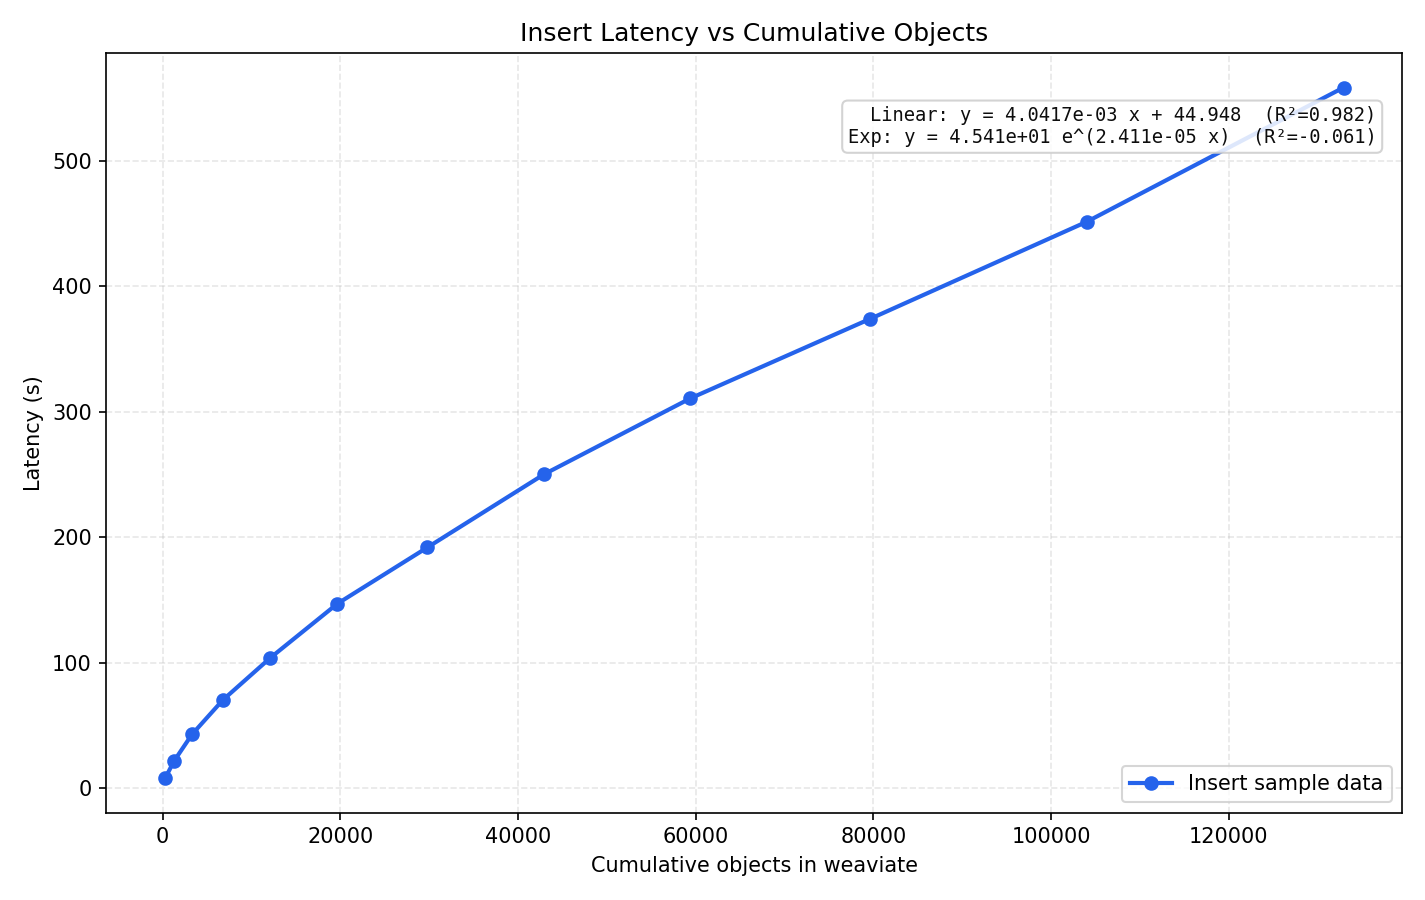
\includegraphics[width=0.32\linewidth]{Figures/insert_latency_vs_files.png}%
        \label{fig:insert-latency-vs-files}%
    }
    \hfill
    \subfigure[Query latency vs. files]{%
        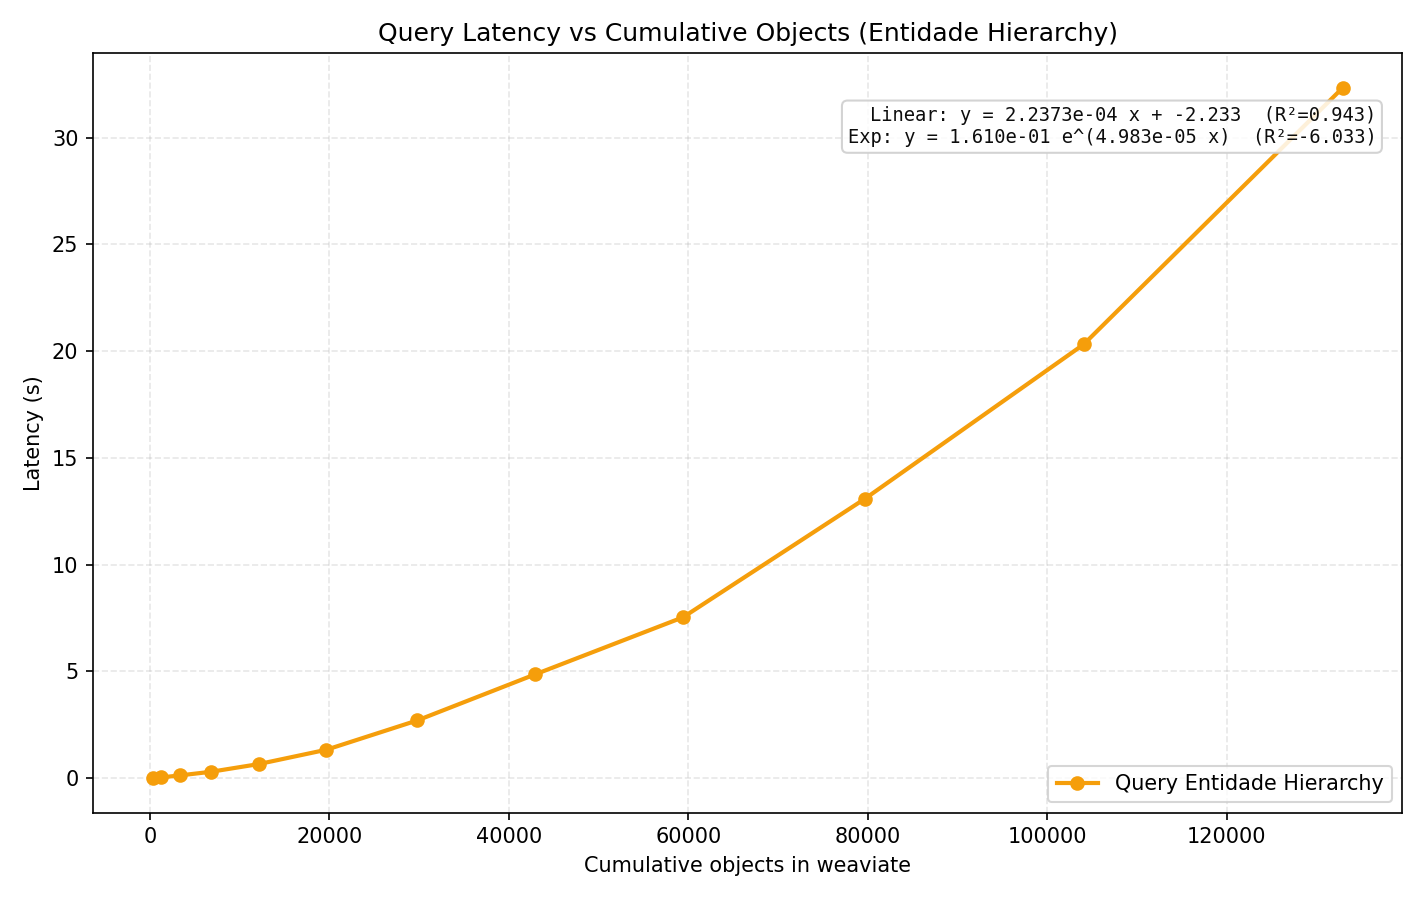
\includegraphics[width=0.32\linewidth]{Figures/query_latency_vs_files.png}%
        \label{fig:query-latency-vs-files}%
    }
    \hfill
    \subfigure[Global semantic search vs. total files]{%
        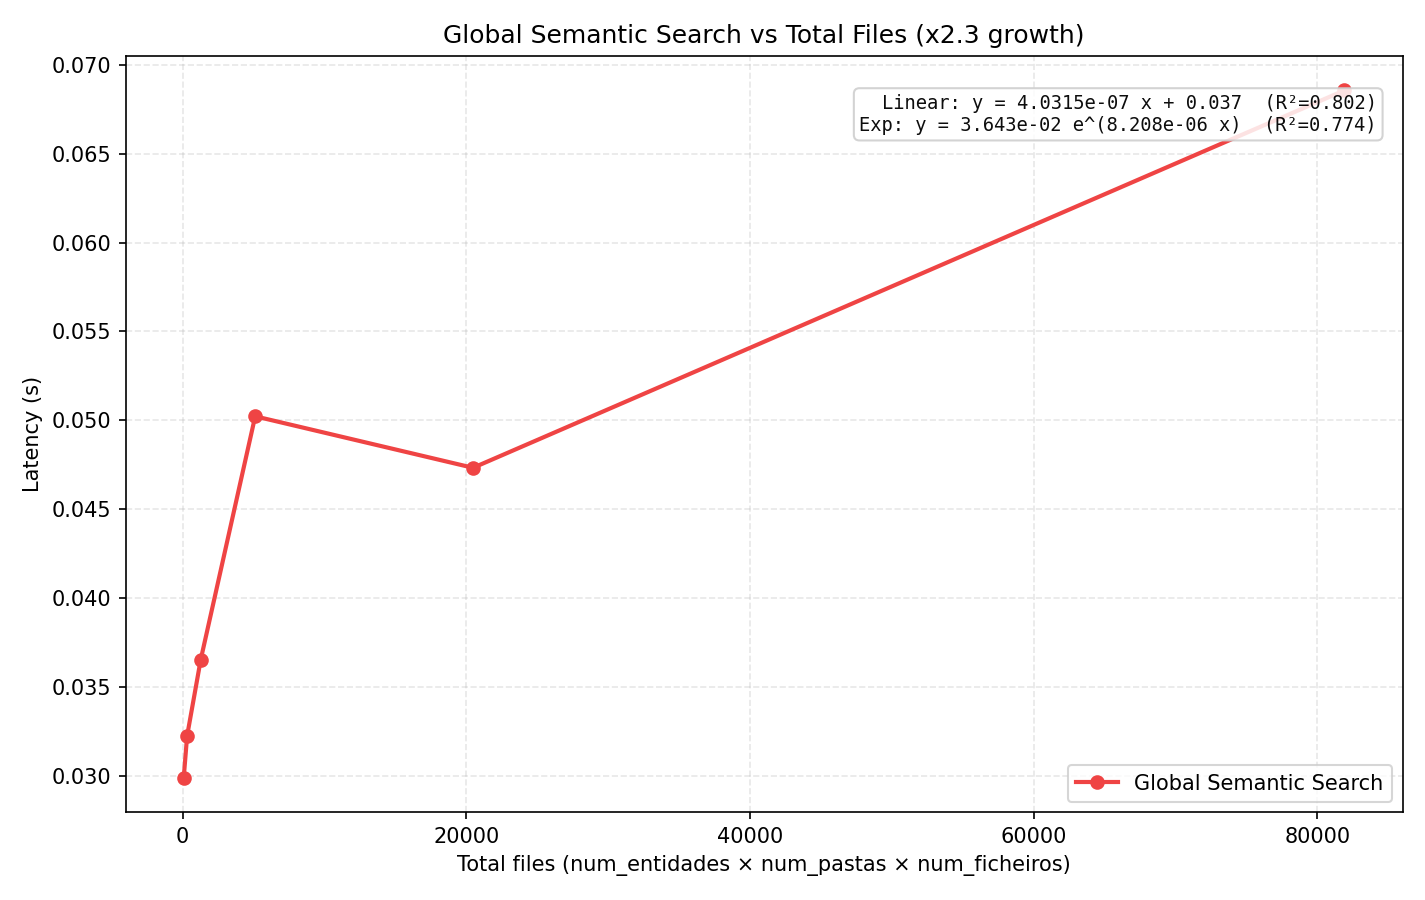
\includegraphics[width=0.32\linewidth]{Figures/semantic_latency_vs_files.png}%
        \label{fig:global-semantic-search-vs-total-files}%
    }
    \caption{Latency and scalability results measured on our Weaviate setup: (a) Insert Latency vs Number of Files showing x577.5 growth with both linear and exponential trend fits and their associated $R^2$ values; (b) Query Latency vs Number of Files comparing a structured traversal (Fluxo $\rightarrow$ Etapas) to an Entidade hierarchy query—note that only the Entidade hierarchy exhibits exponential growth due to cross-reference fan-out, going four layers deep, while Fluxo$\rightarrow$Etapas remains stable; (c) Global semantic search latency as total files increase, showing x2.3 growth and remaining relatively flat.}
\end{figure}

This section validates the practical value of cross-references by running two complementary tests on a compact, real-world–styled example: a structured Weaviate traversal demo and an \gls{ARAG} workflow that follows references via our developed \gls{MCP} server from Section~\ref{sec:weaviate-mcp-server}. 

 
\noindent\textbf{Realistic newsroom setting.} The example intentionally imitates how an international journalism company operates: frontline journalists and editors continuously file reports into the database according to the company's standards for maintaining organization in a highly scalable, dynamic environment. Requiring journalists to provide minimal structured metadata at submission time enables reliable traversal later. A typical filing flow is:
\begin{enumerate}
    \item inserts the document by filing the report as a \textit{Ficheiro} (with title, body, date);
    \item adds the topic in \textit{Fluxo} (storyline) and links the report to it;
    \item records people/organizations/countries in \textit{Entidade} and links them to the report (and stages when relevant);
    \item captures the event/tagging as an \textit{Etapa} (date, category, event) linked to the topic and the report.
\end{enumerate}

Cross-references transform the corpus from a flat, tag-based catalogue into a navigable graph. Unlike standard metadata tagging or hierarchical folder structures, graph organization is dynamic and traversable in high dimensions: edges encode who/what/where/when/etc. and enable deterministic multi-hop traversals. This design also benefits agentic systems by keeping context windows small—retrieving only the minimal set of linked nodes rather than entire files—thereby reducing token usage and latency. We adopt a newsroom scenario because editorial workflows align naturally with this structure: What is the news (\textit{Ficheiro})? To which storyline does it belong (\textit{Fluxo})? Who is involved (\textit{Entidade})? When did it occur (\textit{Etapa})? Keeping the example compact allows us to demonstrate how explicit edges yield grounded, auditable answers. Importantly, structure-aware retrieval improves explainability, trust, and compliance; it reduces ambiguity and accelerates handoffs in high-stakes environments. The schema mirrors the UML in Figure~\ref{fig:weaviate_class} and illustrates how explicit relationships complement semantic search, improving precision without sacrificing flexibility. In production deployments, schemas typically include additional classes and relationships; here we intentionally keep the model small to foreground the core functionality.

\subsection{Structured Demo in Weaviate (Deterministic Traversal)}
\label{subsec:weaviate-xref-structured}

We implemented a minimal newsroom graph using UML classes from Figure~\ref{fig:weaviate_class} that mirrors a common editorial workflow using four classes and cross-references. This graph is dynamic and extensible—edges and nodes can be added as needed to capture new relationships. We omitted the \textit{Pasta} (Folder) class because it is not required for this example. 
The four classes and their key properties/references are:
\begin{itemize}
    \item \textbf{Entidade} (entity): countries, people, organizations; \texttt{hasReports} \(\rightarrow\) \textit{Ficheiro}
    \item \textbf{Ficheiro} (report/file): title, body, date; \texttt{hasEntidades} \(\rightarrow\) \textit{Entidade}, \texttt{belongsToFluxo} \(\rightarrow\) \textit{Fluxo}, \texttt{triggersEtapas} \(\rightarrow\) \textit{Etapa}
    \item \textbf{Fluxo} (topic/storyline): name, description; \texttt{hasStages} \(\rightarrow\) \textit{Etapa}, \texttt{hasReports} \(\rightarrow\) \textit{Ficheiro}
    \item \textbf{Etapa} (stage/event): name, date, description, category; \texttt{belongsToFluxo} \(\rightarrow\) \textit{Fluxo}, \texttt{aboutReports} \(\rightarrow\) \textit{Ficheiro}, \texttt{aboutEntities} \(\rightarrow\) \textit{Entidade}
\end{itemize}

The demo starts by illustrating how a journalist reports: they insert their document and then add information around it—\textit{Entidade} (who is involved), \textit{Fluxo} (topic/storyline), and \textit{Etapa} (event/date). It then inserts one topic (\enquote{Russia vs Ukraine War}), a report (\enquote{Drone attack hits military base}), entities (\enquote{Russia}, \enquote{Ukraine}, and a journalist \enquote{Jane Doe}), and a stage (\enquote{Destruction of a military base}, category \texttt{war\_crime}). It links objects along the graph edges so traversal is possible.

\begin{quote}
\enquote{Ficheiro.title}: \enquote{Drone attack hits military base} \quad \enquote{Ficheiro.date}: \enquote{2024-07-12T00:00:00Z}\\
\enquote{Fluxo.name}: \enquote{Russia vs Ukraine War}\\
\enquote{Entidade.name}: \enquote{Russia}, \enquote{Ukraine}, \enquote{Jane Doe} (role: \enquote{Journalist})\\
\enquote{Etapa.name}: \enquote{Destruction of a military base} \quad (category: \enquote{war\_crime}; date: \enquote{2024-07-12T00:00:00Z})
\end{quote}

For the complete insertion listing with all fields and cross-references, see Appendix~\ref{chapter:appendixA}, Section~\ref{app:newsroom-insertion}.

\noindent\textit{In practice.} This structure enables immediate, deterministic traversals that answer common newsroom questions:
\begin{itemize}
    \item \textbf{Topic status:} Load the \textit{Fluxo}, follow \texttt{hasStages} and \texttt{hasReports}, sort stages by \texttt{date} client-side, and return the latest stage and report count.
    \item \textbf{Latest war crime:} From the \textit{Fluxo}, traverse \texttt{hasStages} and filter \textit{Etapa} by \texttt{category = war\_crime}; pick the most recent by \texttt{date}.
    \item \textbf{Who reported?:} From the latest \textit{Etapa}, follow \texttt{aboutReports} $\rightarrow$ \textit{Ficheiro} and then \texttt{hasEntidades} to extract people whose \texttt{role} contains \enquote{Journalist}.
    \item \textbf{Start anywhere:} Use hybrid search (BM25 + vectors) on any class to find an entry point (e.g., report, entity, stage), then follow references to aggregate the full context.
\end{itemize}


Process steps mirror the newsroom workflow outlined above, so we omit restating them for brevity. Practically, this structured linking improves retrieval: finding any one of the linked objects (e.g., the report, topic, entity, or stage) is sufficient for the system to follow references and surface all related context. This reduces reliance on text-only retrieval and enables fast, explainable navigation across the repository.

\noindent\textit{Outcome (qualitative).} Because relationships are explicit, these questions are answered by graph navigation rather than free-text similarity. For the inserted example, \texttt{topic\_status} returns the most recent stage; \texttt{latest\_war\_crime} yields the staged event tagged as \texttt{war\_crime}; and \texttt{reporters\_for\_latest\_stage} surfaces the journalist linked to the report that triggered that stage. Hybrid search provides a flexible fallback and a cross-class discovery view, but the multi-hop answers are grounded by references.
Although illustrative, the foregoing results are obtained with manually engineered queries—a capability long established in relational database systems. The next subsection evaluates whether an autonomous agent can exploit these references programmatically. Agent-mediated traversal of references is comparatively more novel and potentially more powerful, as it enables autonomous planning and execution over the graph rather than reliance on fixed, hand-coded traversals. 
\subsection{Agentic RAG over Cross-References (Tool-using ReAct)}
\label{subsec:agentic-xref}
To test whether an agent can leverage cross-references programmatically, we implemented a ReAct-style agent using OpenAI SDK that connects to Weaviate via the \gls{MCP} server developed in this work (Section~\ref{sec:weaviate-mcp-server}). The agent uses a system prompt instructing it to request \enquote{weaviate-origin} and \enquote{weaviate-follow-ref} tools when it needs data and to extract key fields from results. It maintains a persistent session (SQLite) and includes retry/backoff logic.

The agent is asked the same three questions as in the structured demo:
\begin{enumerate}
    \item \enquote{How is the war on Russia and Ukraine?}
    \item \enquote{What is the latest war crime?}
    \item \enquote{Who reported?}
\end{enumerate}
Under the hood, the agent plans, issues a reference-origin query (e.g., load the \textit{Fluxo}), follows references (e.g., \texttt{hasStages} \(\rightarrow\) \textit{Etapa}, \texttt{aboutReports} \(\rightarrow\) \textit{Ficheiro}, \texttt{hasEntidades} \(\rightarrow\) \textit{Entidade}), inspects properties (\texttt{date}, \texttt{category}, \texttt{role}), and produces a concise, grounded answer. Ordered navigation traces for these questions are provided in Appendix~\ref{app:agentic-navigation-traces}, and a graph visualization of this example is provided in Appendix~\ref{fig:schema-example}.
Connectivity checks, Windows-specific event loop policy, and transport selection (stdio or HTTP) are handled by the script.

\noindent\textit{Outcome (qualitative).} On the inserted example, the agent retrieves the topic status, identifies the most recent war-crime stage, and extracts the reporter by following references, matching the deterministic traversal results via tool calls. This validates that cross-references are usable not only by handcrafted queries but also by an autonomous planner that reasons over the graph.

\subsection{Takeaways and Scope}
Cross-references provide the \emph{relational glue} required for multi-hop questions: latest-by-date, filtered-by-category, \enquote{who caused/reported what}, and similar patterns. In the structured setting (Section~\ref{subsec:weaviate-xref-structured}), answers are repeatable and explainable because they follow explicit edges. In the agentic setting (Section~\ref{subsec:agentic-xref}), the same edges become \emph{tools} that an \gls{LLM} can call to plan-and-execute traversals. 

\textbf{Limitation acknowledgment:} This section presents a qualitative validation using a single hand-crafted newsroom example to demonstrate functional correctness. We did not conduct a large-scale quantitative evaluation (measuring retrieval accuracy, precision, or recall over a benchmark dataset) for two reasons: (i) no public benchmark exists for evaluating agentic cross-reference traversal in structured enterprise repositories, and (ii) creating a synthetic benchmark with sufficient complexity and diversity was beyond the scope and budget constraints of this thesis. Future work should develop standardized benchmarks for structure-aware agentic retrieval to enable rigorous comparative evaluation.

Despite this limitation, these tests successfully demonstrate integration readiness and functional correctness: the schema supports reference navigation, and the agent can exploit it to produce grounded, auditable answers. The ordered navigation traces in Appendix~\ref{app:agentic-navigation-traces} show that the system correctly follows cross-references to answer multi-hop questions, validating the core architectural contribution.


% Finally, the summarization techniques were also evaluated in the mixed dataset from Section~\ref{sec:agentic-retrieval-multiple}, combining both LiHua-World and synthetic company questions. The same naive RAG pipeline (using \texttt{qwen2.5m} for generation) was run on the mixed 400-question benchmark, using the same Weaviate collections with summarized documents. In this case the collections were merged in to one, as the decision making of a agent is not relevant in this experiment. The goal of this experiment, is evaluating the impact of summarization techniques in a mixed dataset scenario.

% The results are presented in table~\ref{tab:document_retrieved_metrics_mixed}.
% \begin{table}[t]
% \centering
% \caption{Document retrieval and summarization metrics using mixed dataset from Section~\ref{sec:agentic-retrieval-multiple}}
% \label{tab:document_retrieved_metrics_mixed}
% \begin{tabular}{lrrr}
% \hline
% Approach & Avg. Retrieval Rate & token recall & jaccard \\
% \hline
% MixedLiHua & 46.5\% & 15.8\% & 1.27\% \\
% MixedTotal & 39.4\% & 24.6\% & 19.3\% \\
% LexRank & 33.6\% & 29.5\%  & 35.9\% \\
% MixedSynthetic & 33.0\% & 31.5\% & 33.5\% \\
% \hline
% \end{tabular}
% \end{table}

% The results show that summarization techniques need to be carefully considered. As the Lihua-World benchmark, Avg. Retrieval Rate is high, the answer quality is poor. This happens because the Lihua-World dataset, is dialogues snippets, of a fictional story. Where details are more hidden. Therefore, LexRank summarization ended up removing 
% If Printing on DOUBLE SIDED pages, the second page should be white.
% Otherwise, comment the following command:
\cleardoublepage
%
%Chapter 6
% #############################################################################
% This is Chapter 6
% !TEX root = ../main.tex
% #############################################################################
% Change the Name of the Chapter i the following line
\fancychapter{Conclusion}
\cleardoublepage%
% The following line allows to ref this chapter
\label{chap:conclusion}%


% #############################################################################
\section{Conclusions}

This thesis examined strategies to enhance semantic search by integrating retrieval, large language models, structure-aware system design, and agentic workflows. The findings demonstrate that carefully engineered prompting, robust reasoning strategies, and precise grounding in external knowledge sources significantly improve retrieval and answer quality.

This thesis proposes a design for structure-aware systems that exploit an organization's inherent information structure—including cross-references, collection descriptions, and metadata—to inform and constrain retrieval processes. Although large-scale empirical evaluation was beyond the project's scope, the analysis indicates that, within enterprise environments, structural signals can meaningfully enhance retrieval precision and interpretability.

Prompt-engineering strategies for automated document analysis were also explored (e.g., metadata extraction, organization structuring suggestions, targeted entity extraction, and summarization). Although initial results were modest due to computational and budget constraints, the approach remains promising and is likely to improve through more efficient optimization, stronger models, and refined tuning or few-shot prompting aligned with the application-specific schema.

\gls{AAI} systems—incorporating planning, retrieval, observation, and reflection—were compared to a naive retrieval-augmented generation \gls{RAG} baseline. Across the evaluated tasks, the agentic approach consistently produced more accurate and contextually answers, highlighting the importance of reasoning frameworks and prompt strategies in making information more accessible and interpretable.

From an engineering perspective, extensive use was made of the Weaviate vector database, which enabled rapid experimentation with configurations and providing a clear path to scalability, reproducibility, and integration of \glspl{ACL} within corporate environments. An \gls{MCP} server was also built to interface with Weaviate, enabling standard \gls{MCP} clients (e.g., agents and chatbots) to query and traverse the knowledge base (including traversal).

Collectively, this thesis advances \gls{RAG} pipeline techniques for extracting structured information from unstructured documents via systematic prompt engineering. It proposes a structure-aware retrieval design that leverages organizational signals, and delivers an \gls{MCP} server that integrates with a scalable, AI-enabled vector database (Weaviate) to interface with chatbots and tool-using agents—together providing a practical foundation for building more effective and user-friendly information-retrieval systems across domains. Taken together, the results in Chapter~\ref{chap:results} crystallize best practices and configuration guidelines for the schema-aware agent over cross-references in Weaviate—when to favor agentic planning, how to configure hybrid search and top-$k$ parameters, when to enable multi-collection search, and when to apply extractive summarization—so practitioners can deploy the MCP–Weaviate stack in a robust, cost-aware, and accuracy-oriented manner.
% #############################################################################
\section{System Limitations and Future Work}
The primary limitations of this work were computational capacity, financial budget, and data availability. Our local compute was sufficient to run only small open \glspl{LLM}; evaluating stronger models with extended context windows required using hosted APIs. Per-token pricing for hosted \glspl{LLM} (e.g., OpenAI, Google Gemini) kept day-to-day iteration affordable but rendered large-scale ablations and benchmarking prohibitively expensive, which in turn limited the breadth of experiments, the size and complexity of models we could test, and the context-window lengths we could routinely exercise. These constraints also affected the evaluation of document-analysis pipelines: they were comparatively expensive to run and yielded only modest gains in our setting. Finally, the lack of a publicly available dataset tailored to structure-aware retrieval prevented a comprehensive end-to-end assessment, and the specific model choices restrict the generality of our conclusions.

By design, this thesis does not introduce new \gls{ML} or \gls{LLM} architectures. It assumes that contemporary \glspl{LLM} and embedding models are already sufficiently capable for many enterprise applications and will continue to improve primarily through scaling—both in parameter count and context-window lengh. Accordingly, the focus on \gls{RAG} and prompt-engineering strategies that leverage long-context models to produce more accurate and contextually answers—especially for non-expert users who may lack experience in effective prompting \glspl{LLM}.

Future work should:
\begin{itemize}
	\item evaluate stronger base and instruction-tuned models, with extended context windows, on larger and more diverse datasets, to assess scalability and robustness across domains;
	\item develop and release a public benchmark for structure-aware retrieval that captures cross-references, hierarchies, and organizational context, complemented by human-annotated relevance judgments;
	\item systematically compare prompting and reasoning strategies (e.g., self-consistency, tree-of-thought, \textsc{ReAct}) across domains and tasks;
	\item integrate additional external knowledge sources and more robust grounding (e.g., entity linking, schema alignment, knowledge graphs, retrieval-augmented planning), and evaluate hallucination/faithfulness;
	\item study user experience among non-experts via controlled studies, measuring usability, transparency, latency, cost, and confidence calibration;
	\item quantify cost–quality trade-offs and throughput under realistic workloads, including caching, reranking, and distillation for efficiency.
\end{itemize}

These directions would enable a more comprehensive assessment of the architecture and its benefits in real-world deployments.




% If Printing on DOUBLE SIDED pages, the second page should be white.
% Otherwise, comment the following command:
\cleardoublepage
%
% -----------------------------------------------------------------------------
% BIBLIOGRAPHY
% Add the Bibliography to the PDF table of contents (not the document table of contents)
%\pdfbookmark[0]{Bibliography}{bib}
\addcontentsline{toc}{chapter}{Bibliography}
% The bibliography style sheet
% Chose your preferences on the format of the entries and the Labels:
% IEEEtran: Used in general (recommended for IST Thesis)
%           Entries are labelled and sorted by appearance in the document
%           Labels are Numeric inside square brackets
\bibliographystyle{IEEEtran}
%
% Apalike:  Entries formatted alphabetically, last name first, with identation
%           Labels with Autor's Name and Year inside square brackets
%\bibliographystyle{apalike}
%
% Alpha:    Entries formatted with Autor's Name and Year, hanging identation
%           Labels with Autor's abbr. Names and Year inside square brackets
%\bibliographystyle{alpha}
%
% Acm:     Entries formatted with Autor's Name (small Caps), hanging identation
%          Labels are Numeric inside square brackets
%\bibliographystyle{acm}
% The following command resets the 'emphasis' style for bibliography entries
\normalem
% Name of your BiBTeX file
\bibliography{./Thesis-MSc-Bibliography} % Put here your own filename
%
% The following command modifies the 'emphasis' style for bibliography entries
\ULforem
% If Printing on DOUBLE SIDED pages, the second page should be white.
% Otherwise, comment the following command:
\cleardoublepage
%
% -----------------------------------------------------------------------------
% HERE GO THE APPENDIXES IF REQUIRED
% If not required just comment the blocks
\appendix
%% First Appendix
%\pdfbookmark[1]{Appendix A}{appendix}
% #############################################################################
% This is Appendix A
% !TEX root = ../main.tex
% #############################################################################
\chapter{Code of Project}
\label{chapter:appendixA}

Nulla dui purus, eleifend vel, consequat non, dictum porta, nulla. Duis ante mi, laoreet ut, commodo eleifend, cursus nec, lorem. Aenean eu est. Etiam imperdiet turpis. Praesent nec augue. Curabitur ligula quam, rutrum id, tempor sed, consequat ac, dui. Vestibulum accumsan eros nec magna. Vestibulum vitae dui. Vestibulum nec ligula et lorem consequat ullamcorper. 

\begin{lstlisting}[frame=lines,style=XML,caption={Example of a XML file.},label=xmlEx]
<?xml version="1.0" encoding="UTF-8"?>
<StreamInfo version="2.0">
    <Clip duration="PT01M0.00S">
        <BaseURL>videos/</BaseURL>
        <Description>svc_1</Description>
        <Representation mimeType="video/SVC" codecs="svc" frameRate="30.00" bandwidth="401.90"
            width="176" height="144" id="L0">
            <BaseURL>svc_1/</BaseURL>
            <SegmentInfo from="0" to="11" duration="PT5.00S">
                <BaseURL>svc_1-L0-</BaseURL>
            </SegmentInfo>
        </Representation>
        <Representation mimeType="video/SVC" codecs="svc" frameRate="30.00" bandwidth="1322.60"
            width="352" height="288" id="L1">
            <BaseURL>svc_1/</BaseURL>
            <SegmentInfo from="0" to="11" duration="PT5.00S">
                <BaseURL>svc_1-L1-</BaseURL>
            </SegmentInfo>
        </Representation>
    </Clip>
</StreamInfo>
\end{lstlisting}

Etiam imperdiet turpis. Praesent nec augue. Curabitur ligula quam, rutrum id, tempor sed, consequat ac, dui. Maecenas tincidunt velit quis orci. Sed in dui. Nullam ut mauris eu mi mollis luctus. Class aptent taciti sociosqu ad litora torquent per conubia nostra, per inceptos hymenaeos. Sed cursus cursus velit. Sed a massa. Duis dignissim euismod quam.

\begin{spacing}{0.5}
\lstinputlisting[style=coloredASM,language=Assembler,numbers=left,caption={Assembler Main Code.},label=code]
{./tables_and_code/example.asm.txt}
\end{spacing}


Class aptent taciti sociosqu ad litora torquent per conubia nostra, per inceptos hymenaeos. Phasellus eget nisl ut elit porta ullamcorper. Maecenas tincidunt velit quis orci. Sed in dui. Nullam ut mauris eu mi mollis luctus. Class aptent taciti sociosqu ad litora torquent per conubia nostra, per inceptos hymenaeos.

This inline MATLAB code \mcode{for i=1:3, disp('cool'); end;} uses the \verb|\mcode{}| command.\footnote{MATLAB Works also in footnotes: \mcodefn{for i=1:3, disp('cool'); end;}}

Nullam ut mauris eu mi mollis luctus. Class aptent taciti sociosqu ad litora torquent per conubia nostra, per inceptos hymenaeos. Sed cursus cursus velit. Sed a massa. Duis dignissim euismod quam. Nullam euismod metus ut orci.

\begin{lstlisting}[language=matlabfloz,caption={\mcode{Matlab Function}}]
for i = 1:3
	if i >= 5 && a ~= b       % literate programming replacement
		disp('cool');         % comment with some §\mcommentfont\LaTeX in it: $\mcommentfont\pi x^2$§
	end
	[:,ind] = max(vec);
	x_last = x(1,end) - 1;
	v(end);
	ylabel('Voltage (µV)');
end
\end{lstlisting}

Nullam ut mauris eu mi mollis luctus. Class aptent taciti sociosqu ad litora torquent per conubia nostra, per inceptos hymenaeos. Sed cursus cursus velit. Sed a massa. Duis dignissim euismod quam. Nullam euismod metus ut orci.

\lstinputlisting[
	label=lst:matlab_code,
	caption={\mcode{function.m}},
	breaklines=true
	]{./tables_and_code/function.m}

Class aptent taciti sociosqu ad litora torquent per conubia nostra, per inceptos hymenaeos. Phasellus eget nisl ut elit porta ullamcorper. Maecenas tincidunt velit quis orci. Sed in dui. Nullam ut mauris eu mi mollis luctus. Class aptent taciti sociosqu ad litora torquent per conubia nostra, per inceptos hymenaeos. Sed cursus cursus velit. Sed a massa. Duis dignissim euismod quam. Nullam euismod metus ut orci. Vestibulum erat libero, scelerisque et, porttitor et, varius a, leo.

\begin{lstlisting}[style=htmlcssjs,caption={HTML with CSS Code}]
<!DOCTYPE html>
<html>
  <head>
    <title>Listings Style Test</title>
    <meta charset="UTF-8">
    <style>
      /* CSS Test */
      * {
        padding: 0;
        border: 0;
        margin: 0;
      }
    </style>
    <link rel="stylesheet" href="css/style.css" />
  </head>
  <header> hey </header>
  <article> this is a article </article>
  <body>
    <!-- Paragraphs are fine -->
    <div id="box">			
			<p>
			  Hello World
			</p>
      <p>Hello World</p>
      <p id="test">Hello World</p>
			<p></p>
    </div>
    <div>Test</div>
    <!-- HTML script is not consistent -->
    <script src="js/benchmark.js"></script>
    <script>
      function createSquare(x, y) {
        // This is a comment.
        var square = document.createElement('div');
        square.style.width = square.style.height = '50px';
        square.style.backgroundColor = 'blue';
        
        /*
         * This is another comment.
         */
        square.style.position = 'absolute';
        square.style.left = x + 'px'; 
        square.style.top = y + 'px';
        
        var body = document.getElementsByTagName('body')[0];
        body.appendChild(square);
      };
      
      // Please take a look at +=
      window.addEventListener('mousedown', function(event) {
        // German umlaut test: Berührungspunkt ermitteln
        var x = event.touches[0].pageX;
        var y = event.touches[0].pageY;
        var lookAtThis += 1;
      });
    </script>
  </body>
</html>
\end{lstlisting}

Nulla dui purus, eleifend vel, consequat non, dictum porta, nulla. Duis ante mi, laoreet ut, commodo eleifend, cursus nec, lorem. Aenean eu est. Etiam imperdiet turpis. Praesent nec augue. Curabitur ligula quam, rutrum id, tempor sed, consequat ac, dui. Vestibulum accumsan eros nec magna. Vestibulum vitae dui. Vestibulum nec ligula et lorem consequat ullamcorper.

\begin{lstlisting}[style=htmlcssjs,caption={HTML CSS Javascript Code}]

@media only screen and (min-width: 768px) and (max-width: 991px) {
	
	#main {
		width: 712px;
		padding: 100px 28px 120px;
	}
	
	/* .mono {
		font-size: 90%;
	} */
	
	.cssbtn a {
		margin-top: 10px;
		margin-bottom: 10px;
		width: 60px;  
		height: 60px;   
		font-size: 28px;
		line-height: 62px;
	}
\end{lstlisting}

Nulla dui purus, eleifend vel, consequat non, dictum porta, nulla. Duis ante mi, laoreet ut, commodo eleifend, cursus nec, lorem. Aenean eu est. Etiam imperdiet turpis. Praesent nec augue. Curabitur ligula quam, rutrum id, tempor sed, consequat ac, dui. Vestibulum accumsan eros nec magna. Vestibulum vitae dui. Vestibulum nec ligula et lorem consequat ullamcorper.

\begin{lstlisting} [style=py,caption={PYTHON Code}]
class TelgramRequestHandler(object):
    def handle(self):
        addr = self.client_address[0]         # Client IP-adress
        telgram = self.request.recv(1024)     # Recieve telgram
        print "From: %s, Received: %s" % (addr, telgram)
        return
\end{lstlisting}
%% If Printing on DOUBLE SIDED pages, the second page should be white.
%% Otherwise, comment the following command:
\cleardoublepage
%% Second Appendix
%\pdfbookmark[1]{Appendix B}{appendix}
% #############################################################################
% This is Appendix B
% !TEX root = ../main.tex
% #############################################################################
\chapter{A Large Table}
\label{chapter:appendixB}

Aliquam et nisl vel ligula consectetuer suscipit. Morbi euismod enim eget neque. Donec sagittis massa. Vestibulum quis augue sit amet ipsum laoreet pretium. Nulla facilisi. Duis tincidunt, felis et luctus placerat, ipsum libero vestibulum sem, vitae elementum wisi ipsum a metus. Nulla a enim sed dui hendrerit lobortis. Donec lacinia vulputate magna. Vivamus suscipit lectus at quam. In lectus est, viverra a, ultricies ut, pulvinar vitae, tellus. Donec et lectus et sem rutrum sodales. Morbi cursus. Aliquam a odio. Sed tortor velit, convallis eget, porta interdum, convallis sed, tortor. Phasellus ac libero a lorem auctor mattis. Lorem ipsum dolor sit amet, consectetuer adipiscing elit.

Nunc auctor bibendum eros. Maecenas porta accumsan mauris. Etiam enim enim, elementum sed, bibendum quis, rhoncus non, metus. Fusce neque dolor, adipiscing sed, consectetuer et, lacinia sit amet, quam. Suspendisse wisi quam, consectetuer in, blandit sed, suscipit eu, eros. Etiam ligula enim, tempor ut, blandit nec, mollis eu, lectus. Nam cursus. Vivamus iaculis. Aenean risus purus, pharetra in, blandit quis, gravida a, turpis. Donec nisl. Aenean eget mi. Fusce mattis est id diam. Phasellus faucibus interdum sapien. Duis quis nunc. Sed enim.
Nunc auctor bibendum eros. Maecenas porta accumsan mauris. Etiam enim enim, elementum sed, bibendum quis, rhoncus non, metus. Fusce neque dolor, adipiscing sed, consectetuer et, lacinia sit amet, quam.

% Table Example
\newcommand{\greyrow}{\rowcolor[rgb]{0.9,0.9,0.9}}
\newcommand{\whiterow}{\rowcolor[rgb]{1,1,1}}
\newcommand{\greycell}[1]{\multicolumn{1}{{>{\columncolor[rgb]{0.9,0.9,0.9}}c}}{#1}}
\newcommand{\lightgreycell}[1]{\multicolumn{1}{{>{\columncolor[rgb]{0.9,0.9,0.9}}c}}{#1}}
\newcommand{\mediumgreycell}[1]{\multicolumn{1}{{>{\columncolor[rgb]{0.8,0.8,0.8}}c}}{#1}}
\newcommand{\darkgreycell}[1]{\multicolumn{1}{{>{\columncolor[rgb]{0.7,0.7,0.7}}c}}{#1}}
\newcommand{\whitecell}[1]{\multicolumn{1}{{>{\columncolor[rgb]{1,1,1}}c}}{#1}}

\newcommand{\cellformatG}[1]{\multicolumn{1}{{>{\columncolor[rgb]{.9,.9,.9}}c}}{#1}}
\newcommand{\cellformatW}[1]{\multicolumn{1}{{>{\columncolor[rgb]{1,1,1}}c}}{#1}}
\newcommand{\cellformatlG}[1]{\multicolumn{1}{{|>{\columncolor[rgb]{.9,.9,.9}}c}}{#1}}
\newcommand{\cellformatlW}[1]{\multicolumn{1}{{|>{\columncolor[rgb]{1,1,1}}c}}{#1}}
\newcommand{\cellformatrG}[1]{\multicolumn{1}{{>{\columncolor[rgb]{.9,.9,.9}}c|}}{#1}}
\newcommand{\cellformatrW}[1]{\multicolumn{1}{{>{\columncolor[rgb]{1,1,1}}c|}}{#1}}
\newcommand{\cellformatlrG}[1]{\multicolumn{1}{{|>{\columncolor[rgb]{.9,.9,.9}}c|}}{#1}}
\newcommand{\cellformatlrW}[1]{\multicolumn{1}{{|>{\columncolor[rgb]{1,1,1}}c|}}{#1}}

\begin{table}[t]
\centering
\caption{Example table}
\label{table:table1}
\begin{tabular}{c c c c c c}
\hline
\cellformatrG{}&\cellformatlG{}&\cellformatrG{}&\cellformatlG{}&\cellformatrG{}&\cellformatlG{}\\
\cellformatrG{}&
\cellformatlG{\multirow{-2}{*}{\centering\bf \#Layers}} & 
\cellformatrG{\multirow{-2}{*}{\centering\bf \#Nets}} & 
\cellformatlG{\multirow{-2}{*}{\centering \#Nodes\Mark1}} & 
\cellformatrG{\multirow{-2}{1.8cm}{\centering Critical path}}&
\cellformatlG{\multirow{-2}{2cm}{\centering\bf Latency ($T_{iter}$)}}\\
\cellformatrG{\multirow{-3}{2.2cm}{\centering Benchmark: ANN}} &
\cellformatlG{\footnotesize $(1)$} & 
\cellformatrG{\footnotesize$(2)$} & 
\cellformatlG{\footnotesize$(3)=8\cdot(1)\cdot(2)$} & 
\cellformatrG{\footnotesize$(4)=4\cdot(1)$} & 
\cellformatlG{\footnotesize$(5)$}\\
\hline
\cellformatrW{A1} & \cellformatlW{\bf 3--1501} & \cellformatrW{       1   } & \cellformatlW{\bf 24--12008}  & \cellformatrW{\bf 12--6004} & \cellformatlW{    4}\\
\cellformatrW{A2} & \cellformatlW{    501    } & \cellformatrW{       1   } & \cellformatlW{     4008    }  & \cellformatrW{  2004      } & \cellformatlW{\bf 2--2000 }\\
\cellformatrW{A3} & \cellformatlW{     10    } & \cellformatrW{\bf 2--1024} & \cellformatlW{\bf 160--81920} & \cellformatrW{    40      } & \cellformatlW{   60\Mark2 }\\
\cellformatrW{A4} & \cellformatlW{     10    } & \cellformatrW{      50   } & \cellformatlW{     4000    }  & \cellformatrW{    40      } & \cellformatlW{\bf 80--1200}\\
\hline
\multicolumn{6}{c}{\vspace*{-0.3cm}}\\
%%%%%%%%%%%%% SECOND PART OF THE TABLE %%%%%%%%%%%%%%%%%%%%%%%%
\hline
\cellformatrG{}&\cellformatlG{}&\cellformatrG{}&\cellformatlG{}&\cellformatrG{}&\cellformatlG{}\\
\cellformatrG{}&
\cellformatlG{\multirow{-2}{1.6cm}{\centering\bf FFT size\Mark3}} & 
\cellformatrG{\multirow{-2}{*}{\centering\it\#Inputs}} & 
\cellformatlG{\multirow{-2}{*}{\centering\it \#Nodes\Mark1}} & 
\cellformatrG{\multirow{-2}{1.8cm}{\centering\it Critical path}}&
\cellformatlG{\multirow{-2}{2cm}{\centering\bf Latency ($T_{iter}$)}}\\
\cellformatrG{\multirow{-3}{2.2cm}{\centering Benchmark: FFT}}& 
\cellformatlG{\footnotesize$(1)$} & 
\cellformatrG{\footnotesize$(2)=2^{(1)}$} & 
\cellformatlG{\footnotesize$(3)=10\cdot(1)\cdot (2)$} & 
\cellformatrG{\footnotesize$(4)=4\cdot (1)$} & 
\cellformatlG{\footnotesize$(5)$}\\
\hline
\cellformatrW{F1} & \cellformatlW{\bf 1--10} & \cellformatrW{2--1024} & \cellformatlW{\bf 20--102400} &  \cellformatrW{4--40} & \cellformatlW{6--60\Mark2}\\
\cellformatrW{F2} & \cellformatlW{\bf 5} & \cellformatrW{32} & \cellformatlW{1600} & \cellformatrW{20} & \cellformatlW{\bf 40 -- 1500}\\
\hline
\multicolumn{6}{c}{\vspace*{-0.3cm}}\\
% THIRD AND LAST TABLE!!!
\hline
\cellformatrG{}&\cellformatlG{}&\cellformatrG{}&\cellformatlG{}&\cellformatrG{}&\cellformatlG{}\\
\cellformatrG{}&
\cellformatlG{\multirow{-2}{*}{\centering\bf\#Types}} & 
\cellformatrG{\multirow{-2}{*}{\centering\bf \#Nodes}} & 
\cellformatlG{\multirow{-2}{*}{\centering\it \#Networks}} & 
\cellformatrG{\multirow{-2}{1.8cm}{\centering\it Critical path}}&
\cellformatlG{\multirow{-2}{2cm}{\centering\bf Latency ($T_{iter}$)}}\\
\cellformatrG{\multirow{-3}{2.2cm}{\centering Benchmark: Random networks}}& 
\cellformatlG{\footnotesize$(1)$} & 
\cellformatrG{\footnotesize$(2)$} & 
\cellformatlG{\footnotesize$(3)$} &
\cellformatrG{\footnotesize$(4)$} & 
\cellformatlG{\footnotesize$(5)$}\\
\hline
\cellformatrW{R1} & \cellformatlW{3} & \cellformatrW{10--2000} & \cellformatlW{500} &  \cellformatrW{\it variable} & \cellformatlW{\footnotesize$(4)$}\\
\cellformatrW{R2} & \cellformatlW{3} & \cellformatrW{  50    } & \cellformatlW{500} &  \cellformatrW{\it variable} & \cellformatlW{\footnotesize$(4)\times [1;\cdots;20]$}\\
\hline
\multicolumn{6}{c}{\vspace*{-0.3cm}}\\
\multicolumn{6}{l}{\it\Mark1 Excluding constant nodes.}\\
\multicolumn{6}{l}{\it\Mark2 Value kept proportional to the critical path: $(5)=(4)*1.5$.}\\
\multicolumn{6}{l}{\it\Mark3 A size of $x$ corresponds to a $2^x$ point FFT.}\\
\multicolumn{6}{l}{\it Values in bold indicate the parameter being varied.}
\end{tabular}
\end{table}

\textcolor{violet}{As \Cref{table:table1} shows, the data can be inserted from a file, in the case of a somehow complex structure. Notice the Table footnotes.}	

Lorem ipsum dolor sit amet, consectetuer adipiscing elit. Morbi commodo, ipsum sed pharetra gravida, orci magna rhoncus neque, id pulvinar odio lorem non turpis. Nullam sit amet enim. Suspendisse id velit vitae ligula volutpat condimentum. Aliquam erat volutpat. Sed quis velit. Nulla facilisi. Nulla libero. Vivamus pharetra posuere sapien. Nam consectetuer. Sed aliquam, nunc eget euismod ullamcorper, lectus nunc ullamcorper orci, fermentum bibendum enim nibh eget ipsum. Donec porttitor ligula eu dolor. Maecenas vitae nulla consequat libero cursus venenatis. Nam magna enim, accumsan eu, blandit sed, blandit a, eros. 

\textcolor{violet}{And now an example (\Cref{tab:lon_table}) of a table that extends to more than one page. Notice the repetition of the Caption (with indication that is continued) and of the Header, as well as the continuation text at the bottom.}

\begin{center}
\begin{longtable}{|l|l|l|}
\caption[Example of a very long table spreading in several pages]{Example of a very long table spreading in several pages} \label{tab:lon_table} \\

\hline \multicolumn{1}{|c|}{\textbf{Time (s)}} & \multicolumn{1}{c|}{\textbf{Triple chosen}} & \multicolumn{1}{c|}{\textbf{Other feasible triples}} \\ \hline 
\endfirsthead

\multicolumn{3}{c}%
{{\bfseries \tablename\ \thetable{} -- continued from previous page}} \\
\hline \multicolumn{1}{|c|}{\textbf{Time (s)}} &
\multicolumn{1}{c|}{\textbf{Triple chosen}} &
\multicolumn{1}{c|}{\textbf{Other feasible triples}} \\ \hline 
\endhead

\hline \multicolumn{3}{|r|}{{Continued on next page}} \\ \hline
\endfoot

\hline \hline
\endlastfoot
0 & (1, 11, 13725) & (1, 12, 10980), (1, 13, 8235), (2, 2, 0), (3, 1, 0) \\
2745 & (1, 12, 10980) & (1, 13, 8235), (2, 2, 0), (2, 3, 0), (3, 1, 0) \\
5490 & (1, 12, 13725) & (2, 2, 2745), (2, 3, 0), (3, 1, 0) \\
8235 & (1, 12, 16470) & (1, 13, 13725), (2, 2, 2745), (2, 3, 0), (3, 1, 0) \\
10980 & (1, 12, 16470) & (1, 13, 13725), (2, 2, 2745), (2, 3, 0), (3, 1, 0) \\
13725 & (1, 12, 16470) & (1, 13, 13725), (2, 2, 2745), (2, 3, 0), (3, 1, 0) \\
16470 & (1, 13, 16470) & (2, 2, 2745), (2, 3, 0), (3, 1, 0) \\
19215 & (1, 12, 16470) & (1, 13, 13725), (2, 2, 2745), (2, 3, 0), (3, 1, 0) \\
21960 & (1, 12, 16470) & (1, 13, 13725), (2, 2, 2745), (2, 3, 0), (3, 1, 0) \\
24705 & (1, 12, 16470) & (1, 13, 13725), (2, 2, 2745), (2, 3, 0), (3, 1, 0) \\
27450 & (1, 12, 16470) & (1, 13, 13725), (2, 2, 2745), (2, 3, 0), (3, 1, 0) \\
30195 & (2, 2, 2745) & (2, 3, 0), (3, 1, 0) \\
32940 & (1, 13, 16470) & (2, 2, 2745), (2, 3, 0), (3, 1, 0) \\
35685 & (1, 13, 13725) & (2, 2, 2745), (2, 3, 0), (3, 1, 0) \\
38430 & (1, 13, 10980) & (2, 2, 2745), (2, 3, 0), (3, 1, 0) \\
41175 & (1, 12, 13725) & (1, 13, 10980), (2, 2, 2745), (2, 3, 0), (3, 1, 0) \\
43920 & (1, 13, 10980) & (2, 2, 2745), (2, 3, 0), (3, 1, 0) \\
46665 & (2, 2, 2745) & (2, 3, 0), (3, 1, 0) \\
49410 & (2, 2, 2745) & (2, 3, 0), (3, 1, 0) \\
52155 & (1, 12, 16470) & (1, 13, 13725), (2, 2, 2745), (2, 3, 0), (3, 1, 0) \\
54900 & (1, 13, 13725) & (2, 2, 2745), (2, 3, 0), (3, 1, 0) \\
57645 & (1, 13, 13725) & (2, 2, 2745), (2, 3, 0), (3, 1, 0) \\
60390 & (1, 12, 13725) & (2, 2, 2745), (2, 3, 0), (3, 1, 0) \\
63135 & (1, 13, 16470) & (2, 2, 2745), (2, 3, 0), (3, 1, 0) \\
65880 & (1, 13, 16470) & (2, 2, 2745), (2, 3, 0), (3, 1, 0) \\
68625 & (2, 2, 2745) & (2, 3, 0), (3, 1, 0) \\
71370 & (1, 13, 13725) & (2, 2, 2745), (2, 3, 0), (3, 1, 0) \\
74115 & (1, 12, 13725) & (2, 2, 2745), (2, 3, 0), (3, 1, 0) \\
76860 & (1, 13, 13725) & (2, 2, 2745), (2, 3, 0), (3, 1, 0) \\
79605 & (1, 13, 13725) & (2, 2, 2745), (2, 3, 0), (3, 1, 0) \\
82350 & (1, 12, 13725) & (2, 2, 2745), (2, 3, 0), (3, 1, 0) \\
85095 & (1, 12, 13725) & (1, 13, 10980), (2, 2, 2745), (2, 3, 0), (3, 1, 0) \\
87840 & (1, 13, 16470) & (2, 2, 2745), (2, 3, 0), (3, 1, 0) \\
90585 & (1, 13, 16470) & (2, 2, 2745), (2, 3, 0), (3, 1, 0) \\
93330 & (1, 13, 13725) & (2, 2, 2745), (2, 3, 0), (3, 1, 0) \\
96075 & (1, 13, 16470) & (2, 2, 2745), (2, 3, 0), (3, 1, 0) \\
98820 & (1, 13, 16470) & (2, 2, 2745), (2, 3, 0), (3, 1, 0) \\
101565 & (1, 13, 13725) & (2, 2, 2745), (2, 3, 0), (3, 1, 0) \\
104310 & (1, 13, 16470) & (2, 2, 2745), (2, 3, 0), (3, 1, 0) \\
107055 & (1, 13, 13725) & (2, 2, 2745), (2, 3, 0), (3, 1, 0) \\
109800 & (1, 13, 13725) & (2, 2, 2745), (2, 3, 0), (3, 1, 0) \\
112545 & (1, 12, 16470) & (1, 13, 13725), (2, 2, 2745), (2, 3, 0), (3, 1, 0) \\
115290 & (1, 13, 16470) & (2, 2, 2745), (2, 3, 0), (3, 1, 0) \\
118035 & (1, 13, 13725) & (2, 2, 2745), (2, 3, 0), (3, 1, 0) \\
120780 & (1, 13, 16470) & (2, 2, 2745), (2, 3, 0), (3, 1, 0) \\
123525 & (1, 13, 13725) & (2, 2, 2745), (2, 3, 0), (3, 1, 0) \\
126270 & (1, 12, 16470) & (1, 13, 13725), (2, 2, 2745), (2, 3, 0), (3, 1, 0) \\
129015 & (2, 2, 2745) & (2, 3, 0), (3, 1, 0) \\
131760 & (2, 2, 2745) & (2, 3, 0), (3, 1, 0) \\
134505 & (1, 13, 16470) & (2, 2, 2745), (2, 3, 0), (3, 1, 0) \\
137250 & (1, 13, 13725) & (2, 2, 2745), (2, 3, 0), (3, 1, 0) \\
139995 & (2, 2, 2745) & (2, 3, 0), (3, 1, 0) \\
142740 & (2, 2, 2745) & (2, 3, 0), (3, 1, 0) \\
145485 & (1, 12, 16470) & (1, 13, 13725), (2, 2, 2745), (2, 3, 0), (3, 1, 0) \\
148230 & (2, 2, 2745) & (2, 3, 0), (3, 1, 0) \\
150975 & (1, 13, 16470) & (2, 2, 2745), (2, 3, 0), (3, 1, 0) \\
153720 & (1, 12, 13725) & (2, 2, 2745), (2, 3, 0), (3, 1, 0) \\
156465 & (1, 13, 13725) & (2, 2, 2745), (2, 3, 0), (3, 1, 0) \\
159210 & (1, 13, 13725) & (2, 2, 2745), (2, 3, 0), (3, 1, 0) \\
161955 & (1, 13, 16470) & (2, 2, 2745), (2, 3, 0), (3, 1, 0) \\
164700 & (1, 13, 13725) & (2, 2, 2745), (2, 3, 0), (3, 1, 0) \\
\end{longtable}
\end{center}

An example of a large Table that autofits the size to the page margins is illustrated in \Cref{tab:very-widetab}. Please notice the text size that is shrunken in order fot the table to adjust to the page:

\begin{table}[htbp]
\caption{Sample Table.}\label{tab:very-widetab}
\resizebox{\columnwidth}{!}{\begin{tabular}{|l|l|l|l|l|l|}
\hline
URL &  First Time Visit & Last Time Visit & URL Counts & Value & Reference\\
\hline
https://web.facebook.com/ & 1521241972 & 1522351859 & 177 & 56640 & [facebook-2021]\\
http://localhost/phpmyadmin/ & 1518413861 & 1522075694 & 24 & 39312 & database-management\\
https://mail.google.com/mail/u/ & 1516596003 & 1522352010 & 36 & 33264 & Google-Gmail-2021\\
https://github.com/shawon100& 1517215489 & 1522352266 & 37 & 27528 & Code-Repository\\
https://www.youtube.com/ & 1517229227 & 1521978502 & 24 & 14792 & Youtube-video-2021\\
\hline
\end{tabular}}
\end{table}






%% If Printing on DOUBLE SIDED pages, the second page should be white.
%% Otherwise, comment the following command:
\cleardoublepage

% -----------------------------------------------------------------------------
% And this is THE END of the IST Thesis Document
\end{document}





